\documentclass[11pt,ngerman]{scrartcl}

% standard packages
\usepackage[utf8]{inputenc}  % input in UTF-8
\usepackage[T1]{fontenc}  % output in T1 fonts (westeuropäische Codierung)
\usepackage{lmodern}  % latin modern fonts
\usepackage[ngerman]{babel}  % deutsches Sprachpaket, neue Rechtschreibung

% Seitensetup
\usepackage{scrlayer-scrpage}  % Seitenformatierung durch KOMA-interne Optionen
\usepackage[top=4cm, bottom=4cm]{geometry}  % Seitengeometrie (kann durch KOMA ersetzt werden, hab ich aber nicht geschafft)
\usepackage[hypcap=false]{caption, subcaption}  % caption editing - hypcap warning with hyperref
\usepackage{array}  % table editing

% additional packages
\usepackage{amsmath, amssymb, amstext}  % math packages (American Math Society)
\usepackage{bm}
\usepackage{icomma}  % Kommata in Dezimalzahlen verursachen keinen Abstand mehr
\usepackage{graphicx}  % Bilder einfügen
\usepackage{float} %Bilder placement
\usepackage{pdfpages}  % PDF als vollständige Seiten einfügen
\usepackage{lastpage}  % referenziert die letzte Seite
\usepackage[separate-uncertainty=true]{siunitx}  % bessere Darstellung von Einheiten
\usepackage{makecell} %Dicke Tabellenstriche
\usepackage{longtable}
\usepackage{booktabs}
%\usepackage{datatool}
\usepackage[hidelinks]{hyperref}  % hyperref verlinkt Referenzen - hidelinks entfernt borders um links

% package setups
% Kopf- und Fußzeile durch KOMA
\pagestyle{scrheadings}  % KOMA darf entscheiden
\clearpairofpagestyles  % reset
\setkomafont{pageheadfoot}{\normalfont}  % Standardschrift in Kopf- und Fußzeile
\captionsetup{format=plain, font=small, labelfont=bf} %Better caption, Abbildung ist FETT
%\setlength{\headheight}{27.2pt}  % benötigte Höhe Kopfzeile (warning von scrlayer-scrpage, wird aber automatisch so gerendert, falls diese Option weggelassen wird)
\ihead{Halbleiterdiode}  % Kopf links %Todo Titel ändern
\chead{\textsc{Philipp} Maximilian \\ \textsc{Stark} Matthias}  % Kopf Mitte %Todo Name ändern
\ohead{22 Oktober 2021}  % Kopf rechts %Todo Datum ändern
\cfoot{\pagemark \, / \pageref{LastPage}}  % Fuß Mitte

% Table of Contents
\DeclareTOCStyleEntry{dottedtocline}{section}  % KOMA intern - Inhaltsverzeichnis mit Punkten (nur sections)

%Overbar setup
\newcommand{\overbar}[1]{\mkern 1.5mu\overline{\mkern-1.5mu#1\mkern-1.5mu}\mkern 1.5mu}
% SI
\sisetup{locale = DE}  % deutschsprachige SI-Konvention
\sisetup{quotient-mode = fraction}
\sisetup{per-mode = fraction}
\DeclareSIUnit\px{px}
\DeclareSIUnit\strich{|||}

% citation
\usepackage{csquotes}
\usepackage[backend=biber]{biblatex}
\addbibresource{halbleiter.bib} %Todo .bib befüllen zb.: mit JabRef (Empfehlung der Redaktion)

%Eigene Commands
\newcommand{\der}[2]{\frac{\mathrm{d}#1}{\mathrm{d}#2}}
\newcommand{\pder}[2]{\frac{\partial #1}{\partial #2}}

%\noindent für ges
\setlength{\parindent}{0pt}


\begin{document}
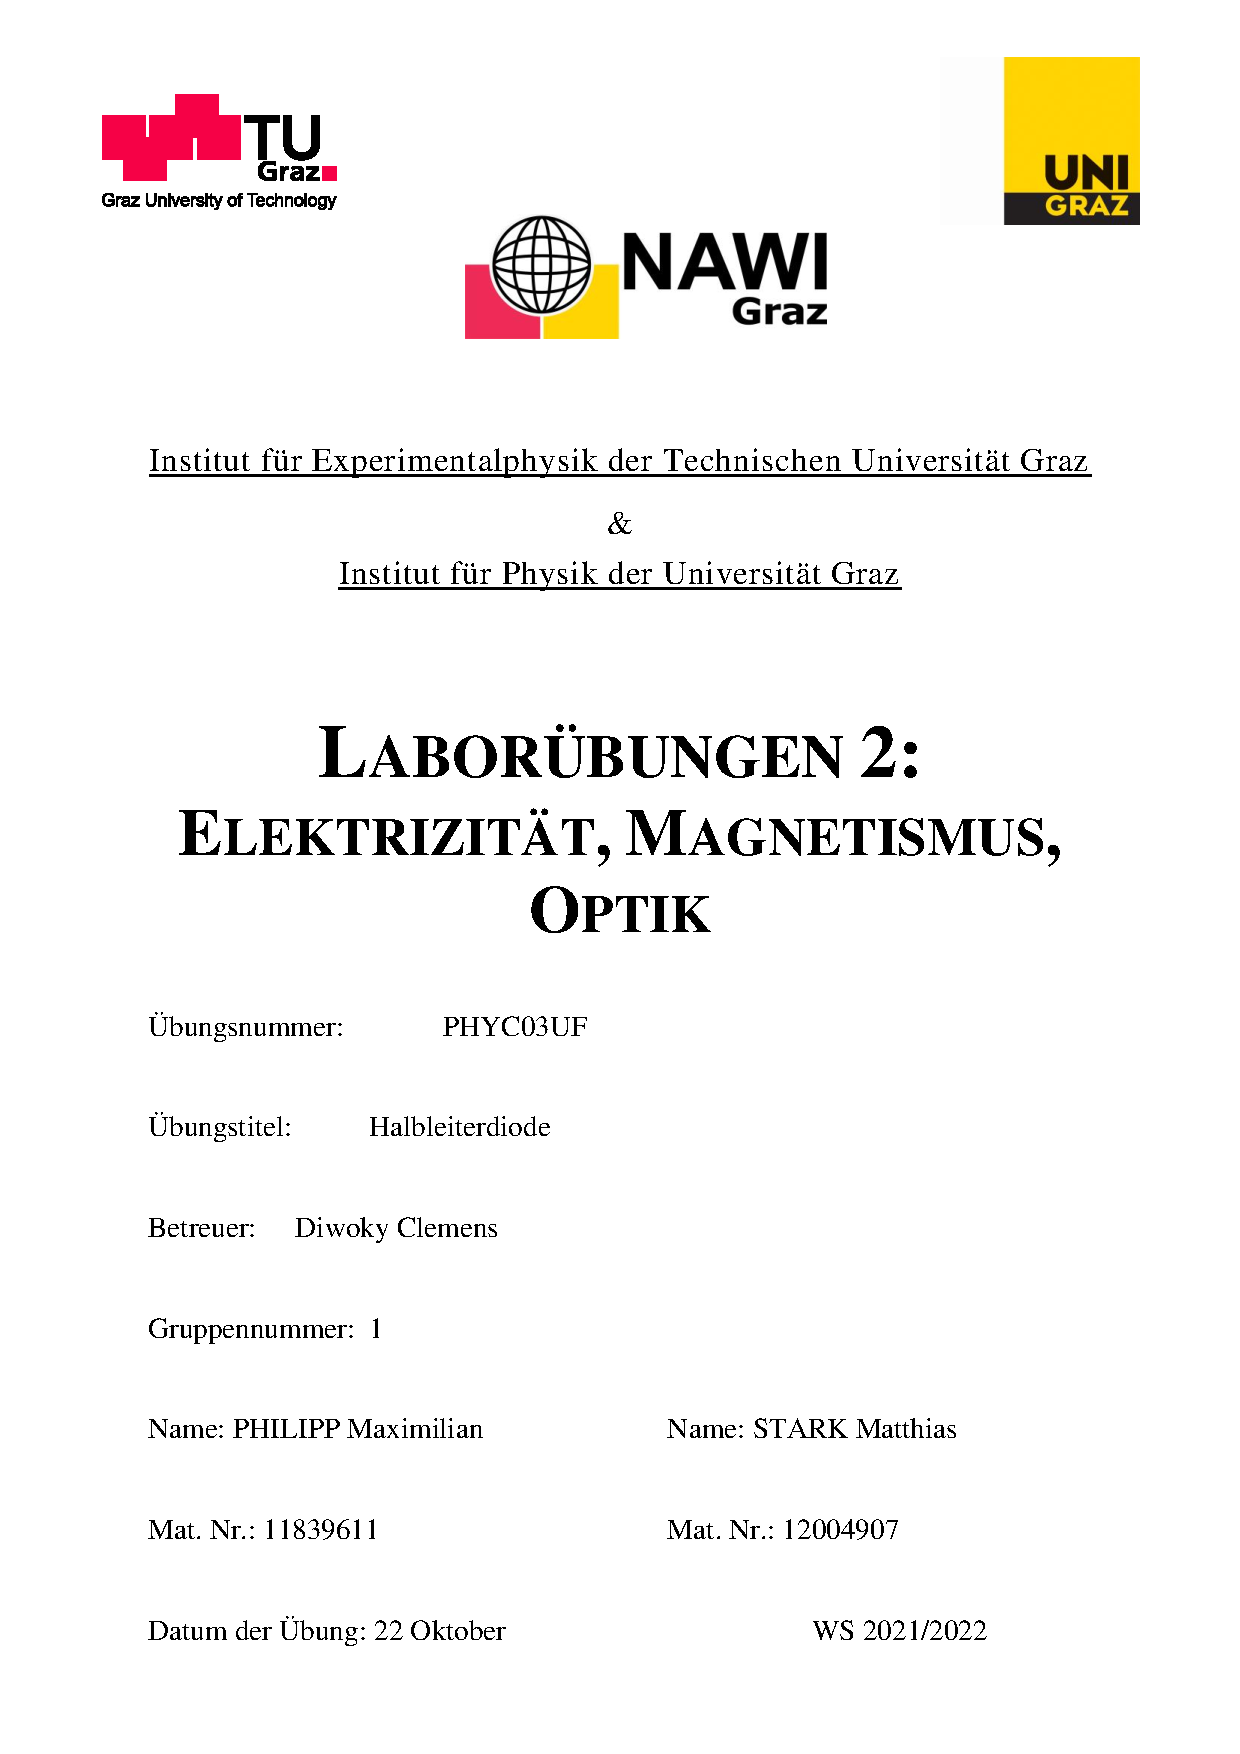
\includepdf{Deckblatt_Stark.pdf}
\tableofcontents
\newpage

\section{Aufgabenstellung\label{Auf0}}

\begin{itemize}
	\item Messtechnische Ermittlung der Strom-Spannungscharakteristik einer Gleichrichterdiode.

	      \subitem a) in Durchlassrichtung

	      \subitem b) in Sperrrichtung

	\item Automatisierte Aufnahme der Strom-Spannungscharakteristik einer Zenerdiode in Durchlass- und Sperrrichtung.

	\item Messtechnische Untersuchung von Spannungs- und Stromverläufen in einer Einweg- Gleichrichterschaltung mit unterschiedlichen Glättungskondensatoren und Belastungswiderständen

	\item Messtechnische Untersuchung von Spannungsverläufen in einer Spannungsverdoppler-Schaltung.
\end{itemize}




\section{Grundlagen}

Unter einem Halbleiter versteht man einen kristallinen Festkörper, dessen Leitfähigkeit zwischen der eines Nichtleiters und der eines Leiters liegt. Die Leitfähigkeit lässt sich anhand des Bändermodells durch freie Ladungsträger erklären, die vom Valenzband über die Bandlücke in das Leitungsband gelangen. Die Menge an Energie, die dafür aufgewendet werden muss, hängt dabei von der Größe der Bandlücke ab und ist in folgender Skizze in \autoref{fig:bander} veranschaulicht.

\begin{center}
	\begin{minipage}[t]{\textwidth}
		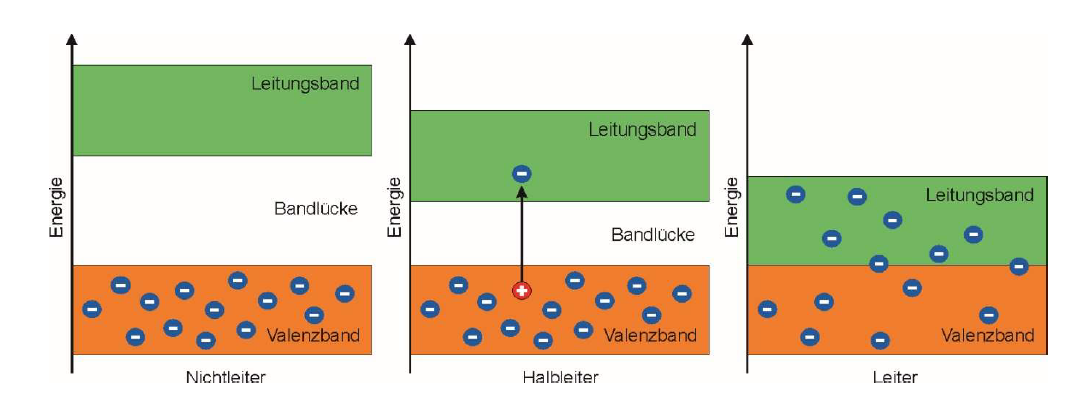
\includegraphics[width=\textwidth]{skizze_bander}
		\captionof{figure}{Skizze des Bändermodells \cite{halbleitervorlage}}
		\label{fig:bander}
	\end{minipage}
\end{center}

Bei den Halbleitern ist die Bandlücke, wie in \autoref{fig:bander} sichtbar, so
klein, dass diese überwunden werden kann. Diese Leitfähigkeit ist allerdings
stark temperaturabhängig. Jedes ins Leitungsband angehobene Elektron
hinterlässt ein positives ``Loch`` im Valenzband, sodass der Halbleiterkristall
insgesamt elektrisch neutral ist.

\vspace{2mm}

Soll nun die Leitfähigkeit der Halbleiterkristallen gezielt verändert werden,
wird dies mit der sogenannten Dotierung erreicht. Darunter versteht man das
Einbringen von Fremdatomen in den Halbleiterkristall. Dabei wird zwischen p-
und n- Dotierung unterschieden.

\vspace{2mm}

Bei der p-Dotierung wird ein Element, welches ein Valenzelektron weniger als der Rest hat, eingebunden, wodurch dieses zu Elektronenakzeptor wird. Die n-Dotierung bewirkt das Gegenteil, wodurch sich durch das zusätzliche Valenzelektron das Valenzband negativ lädt und so zu Elektronendonator wird. Eine schematische Skizze dieses Dotierungsverfahrens von Silizium ist in folgender \autoref{fig:pdot} für die p-Dotierung und in \autoref{fig:ndot} für die n-Dotierung ersichtlich.

\begin{minipage}{\textwidth}
	\begin{minipage}[t]{0.48\textwidth}
		\centering
		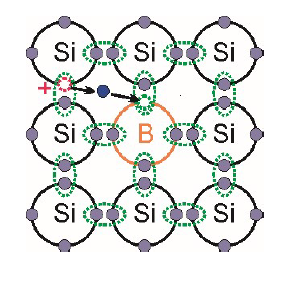
\includegraphics[width=\textwidth]{pdot}
		\captionbelowof{figure}{Skizze von p-Dotierten Silizium \cite{halbleitervorlage}}
		\label{fig:pdot}
	\end{minipage}
	\vspace{2mm}
	\begin{minipage}[t]{0.5\textwidth}
		\centering
		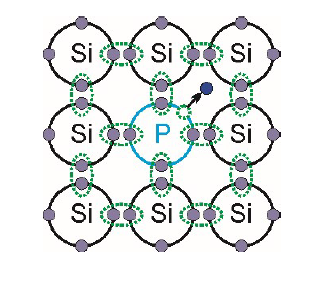
\includegraphics[width=\textwidth]{ndot}
		\captionof{figure}{Skizze von n-Dotierten Silizium \cite{halbleitervorlage}}
		\label{fig:ndot}
	\end{minipage}
	\vspace{1em}
\end{minipage}

Die Stellen des Halbleiterkristalls, an denen der p- und n-dotierte Bereich zusammenkommen, wird p-n Übergang genannt. An der so entstehenden Grenzfläche treten die Elektronen aus dem n-Bereich in den p-Bereich über. In der Sperrschicht entsteht dadurch eine Verarmung an Ladungsträgern, was schließlich zum Verlust der Leitfähigkeit führt.

\vspace{2mm}

Eine Skizze dieses p-n-Übergangs ist in folgender \autoref{fig:pnu} sichtbar.

\begin{center}
	\begin{minipage}[t]{0.65\textwidth}
		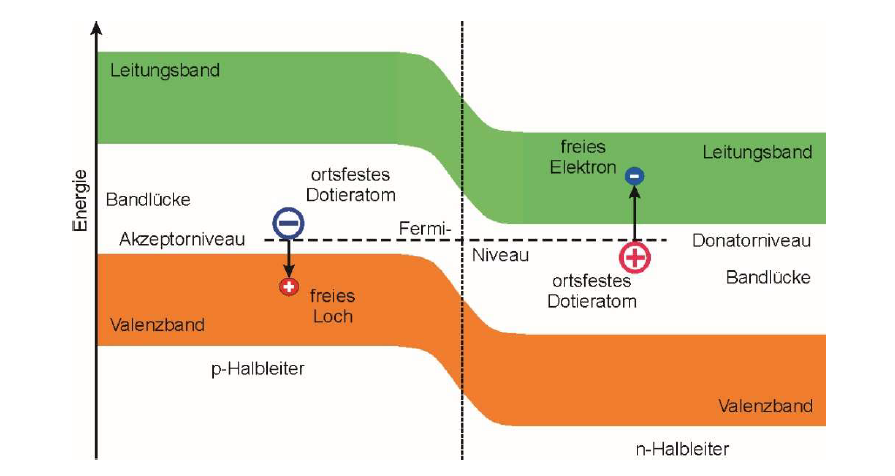
\includegraphics[width=\textwidth]{pnu}
		\captionof{figure}{Skizze des p-n-Übergangs \cite{halbleitervorlage}}
		\label{fig:pnu}
	\end{minipage}
\end{center}

Wird nun der Pluspol einer Spannungsquelle an die p-Dotierte Seite der Halbleiters und der Minuspol an die n-Dotierte Seite geschlossen, fließen die Elektronen zur Raumladungszone, wodurch diese abgebaut wird und so ein Durchlassstrom entsteht.

Wird die Spannungsquelle allerdings mit dem Pluspol zur n-dotierten Seite und mit dem Minuspol zur p-dotierten Seite geschlossen, entfernen sich die Ladungsträger von der Sperrschicht, wodurch diese wächst und so kein Strom fließt, weshalb diese Ausrichtung auch Sperrrichtung der Diode genannt wird. \cite{deimel2015grundlagen} \cite{demtroder2018ex2}



\section{Versuchsanordnung}\label{sec:Versuchsanordnung}

Im Rahmen dieses Versuchs wurden verschiedene Schaltungen dimensioniert. Eine jeweilige Skizze des Schaltplans und eine kurze Erklärung finden sich, der besseren Übersicht halber, immer am Anfang des entsprechenden Versuchs im \autoref{sec:Versuchsdurchführung}.

\vspace{2mm}

Um die Signale für die entsprechenden Schaltpläne zu erzeugen und auszuwerten wurden folgende Geräte verwendet.

\vspace{2mm}

Es handelt sich dabei um einen ``Power Supply``, in \autoref{fig:hameg} und ein Oszilloskop mit 4 Eingängen, siehe \autoref{fig:oszi}

\vspace{2mm}

\begin{minipage}{\textwidth}
	\begin{minipage}[t]{0.5\textwidth}
		\centering
		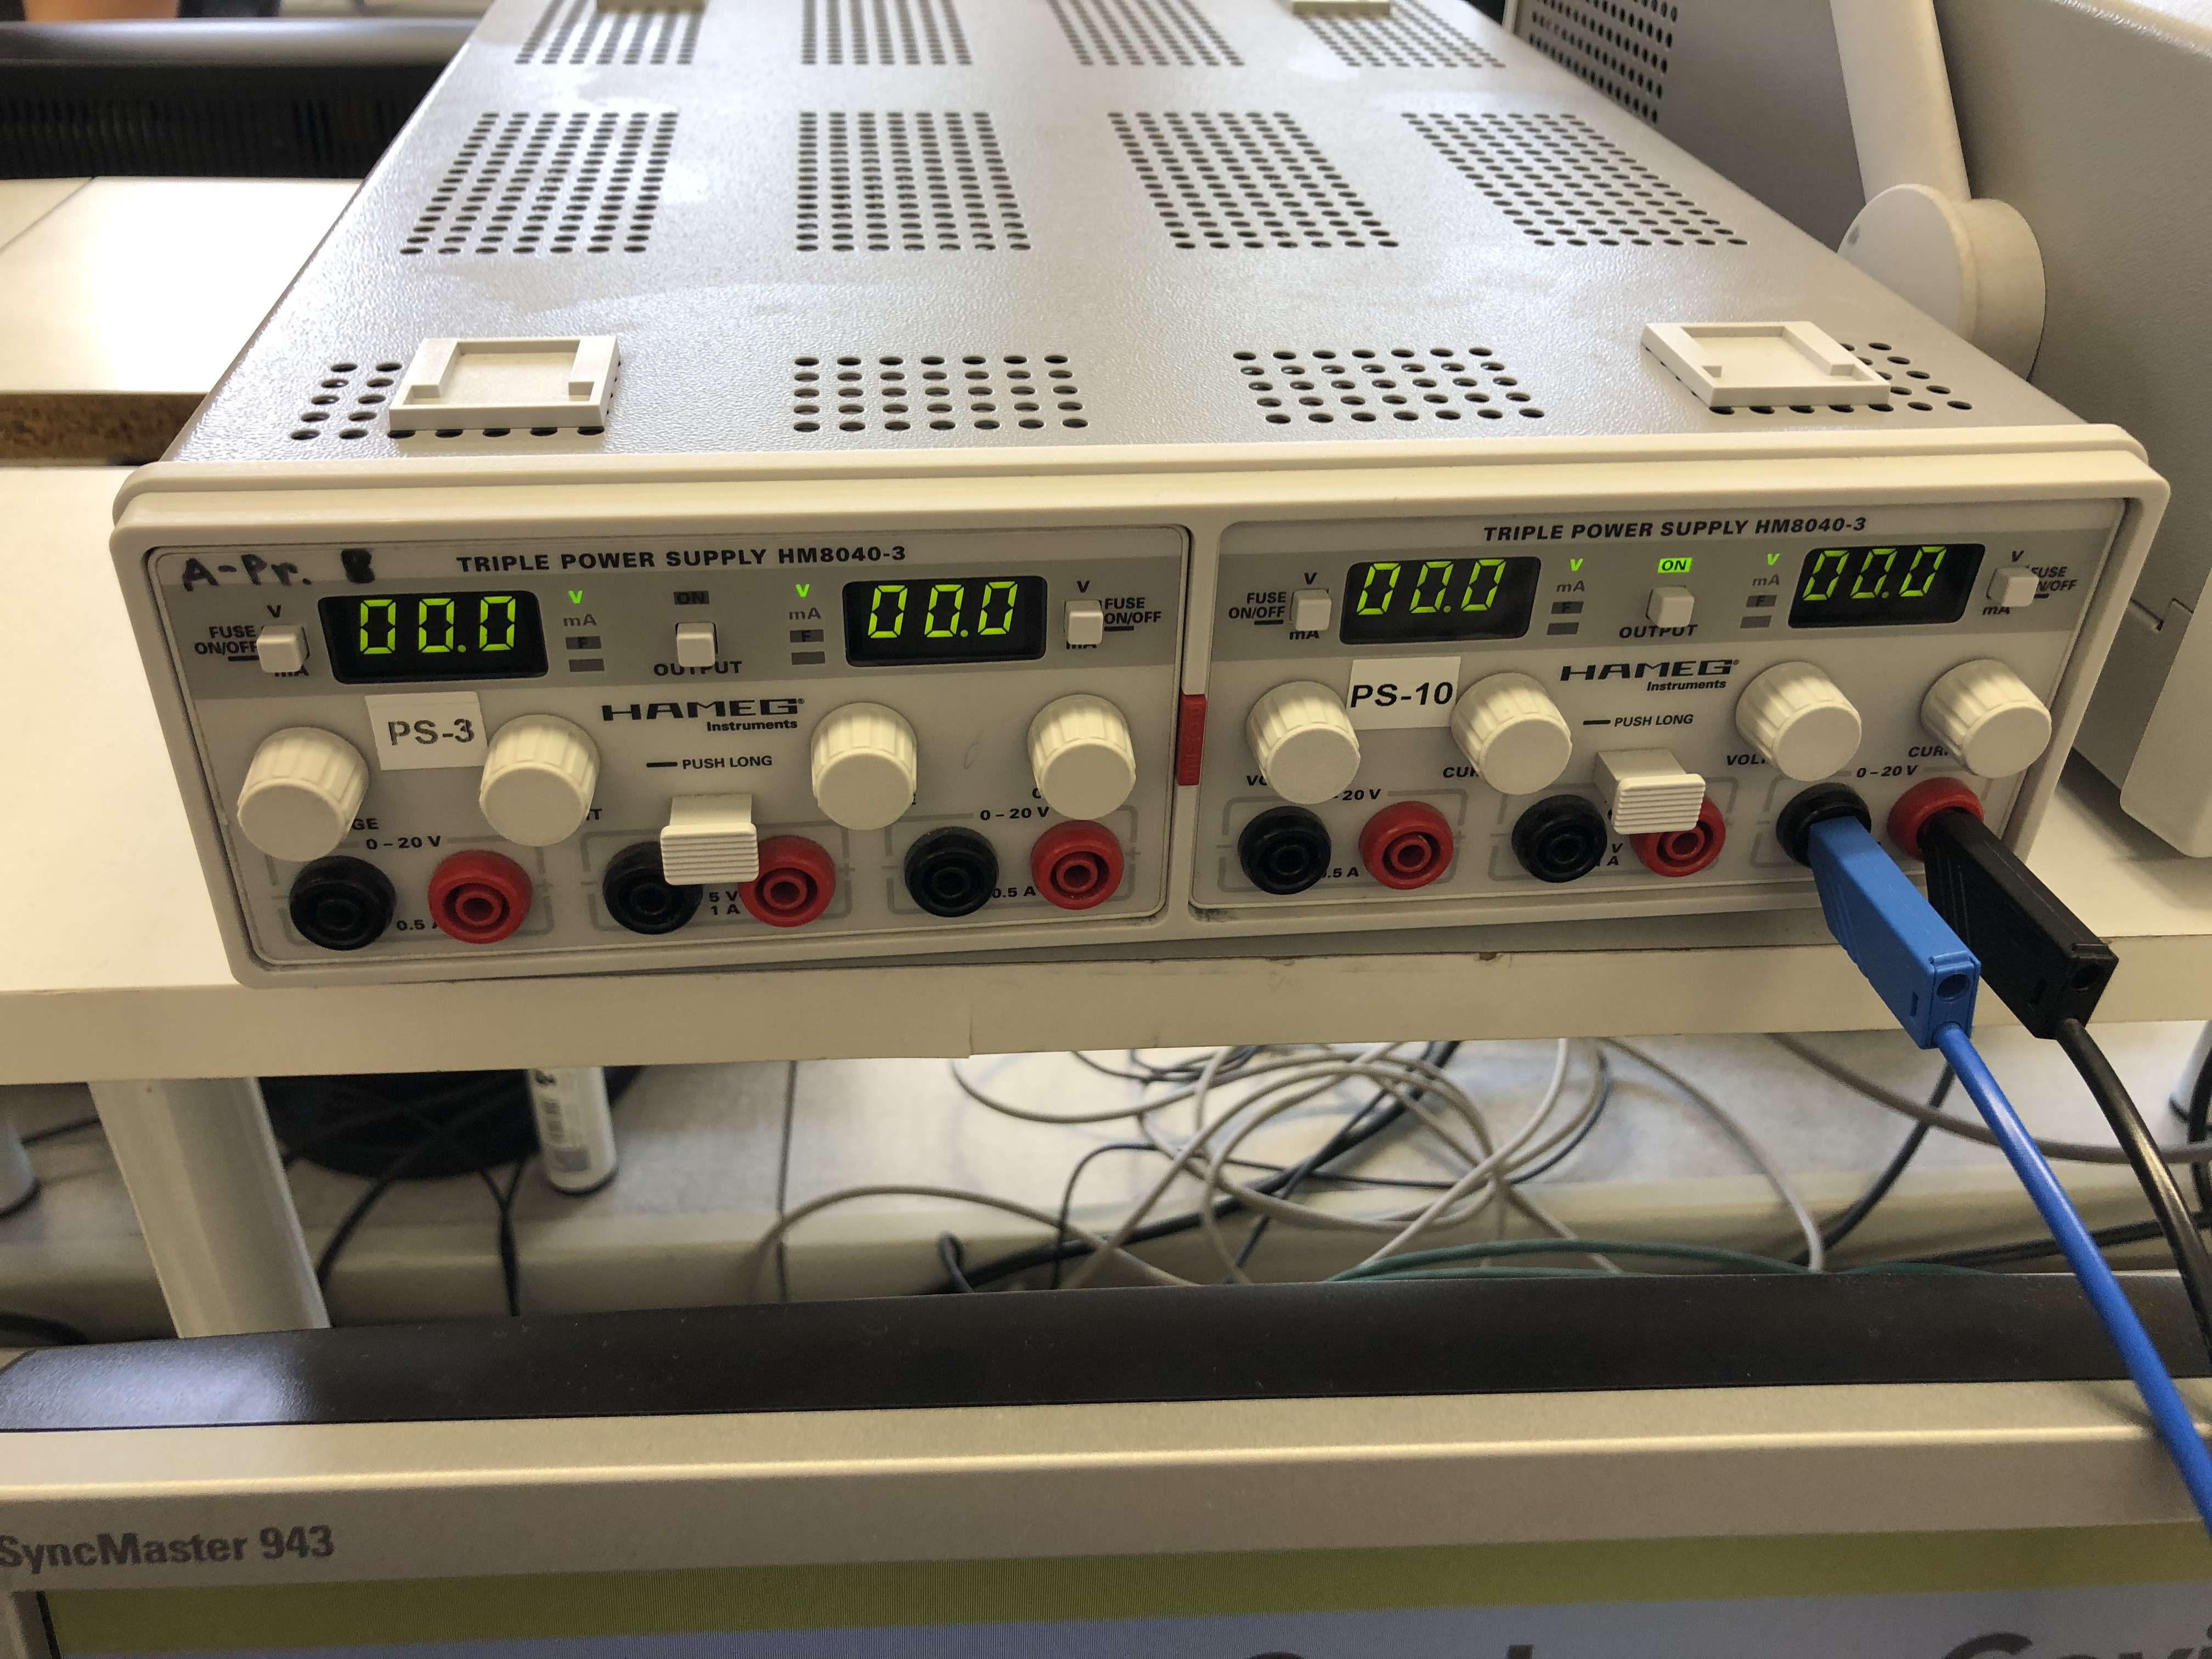
\includegraphics[width=\textwidth]{hameg}
		\captionbelowof{figure}{Verwendeter ``Power Supply``}
		\label{fig:hameg}
	\end{minipage}
	\vspace{2mm}
	\begin{minipage}[t]{0.50\textwidth}
		\centering
		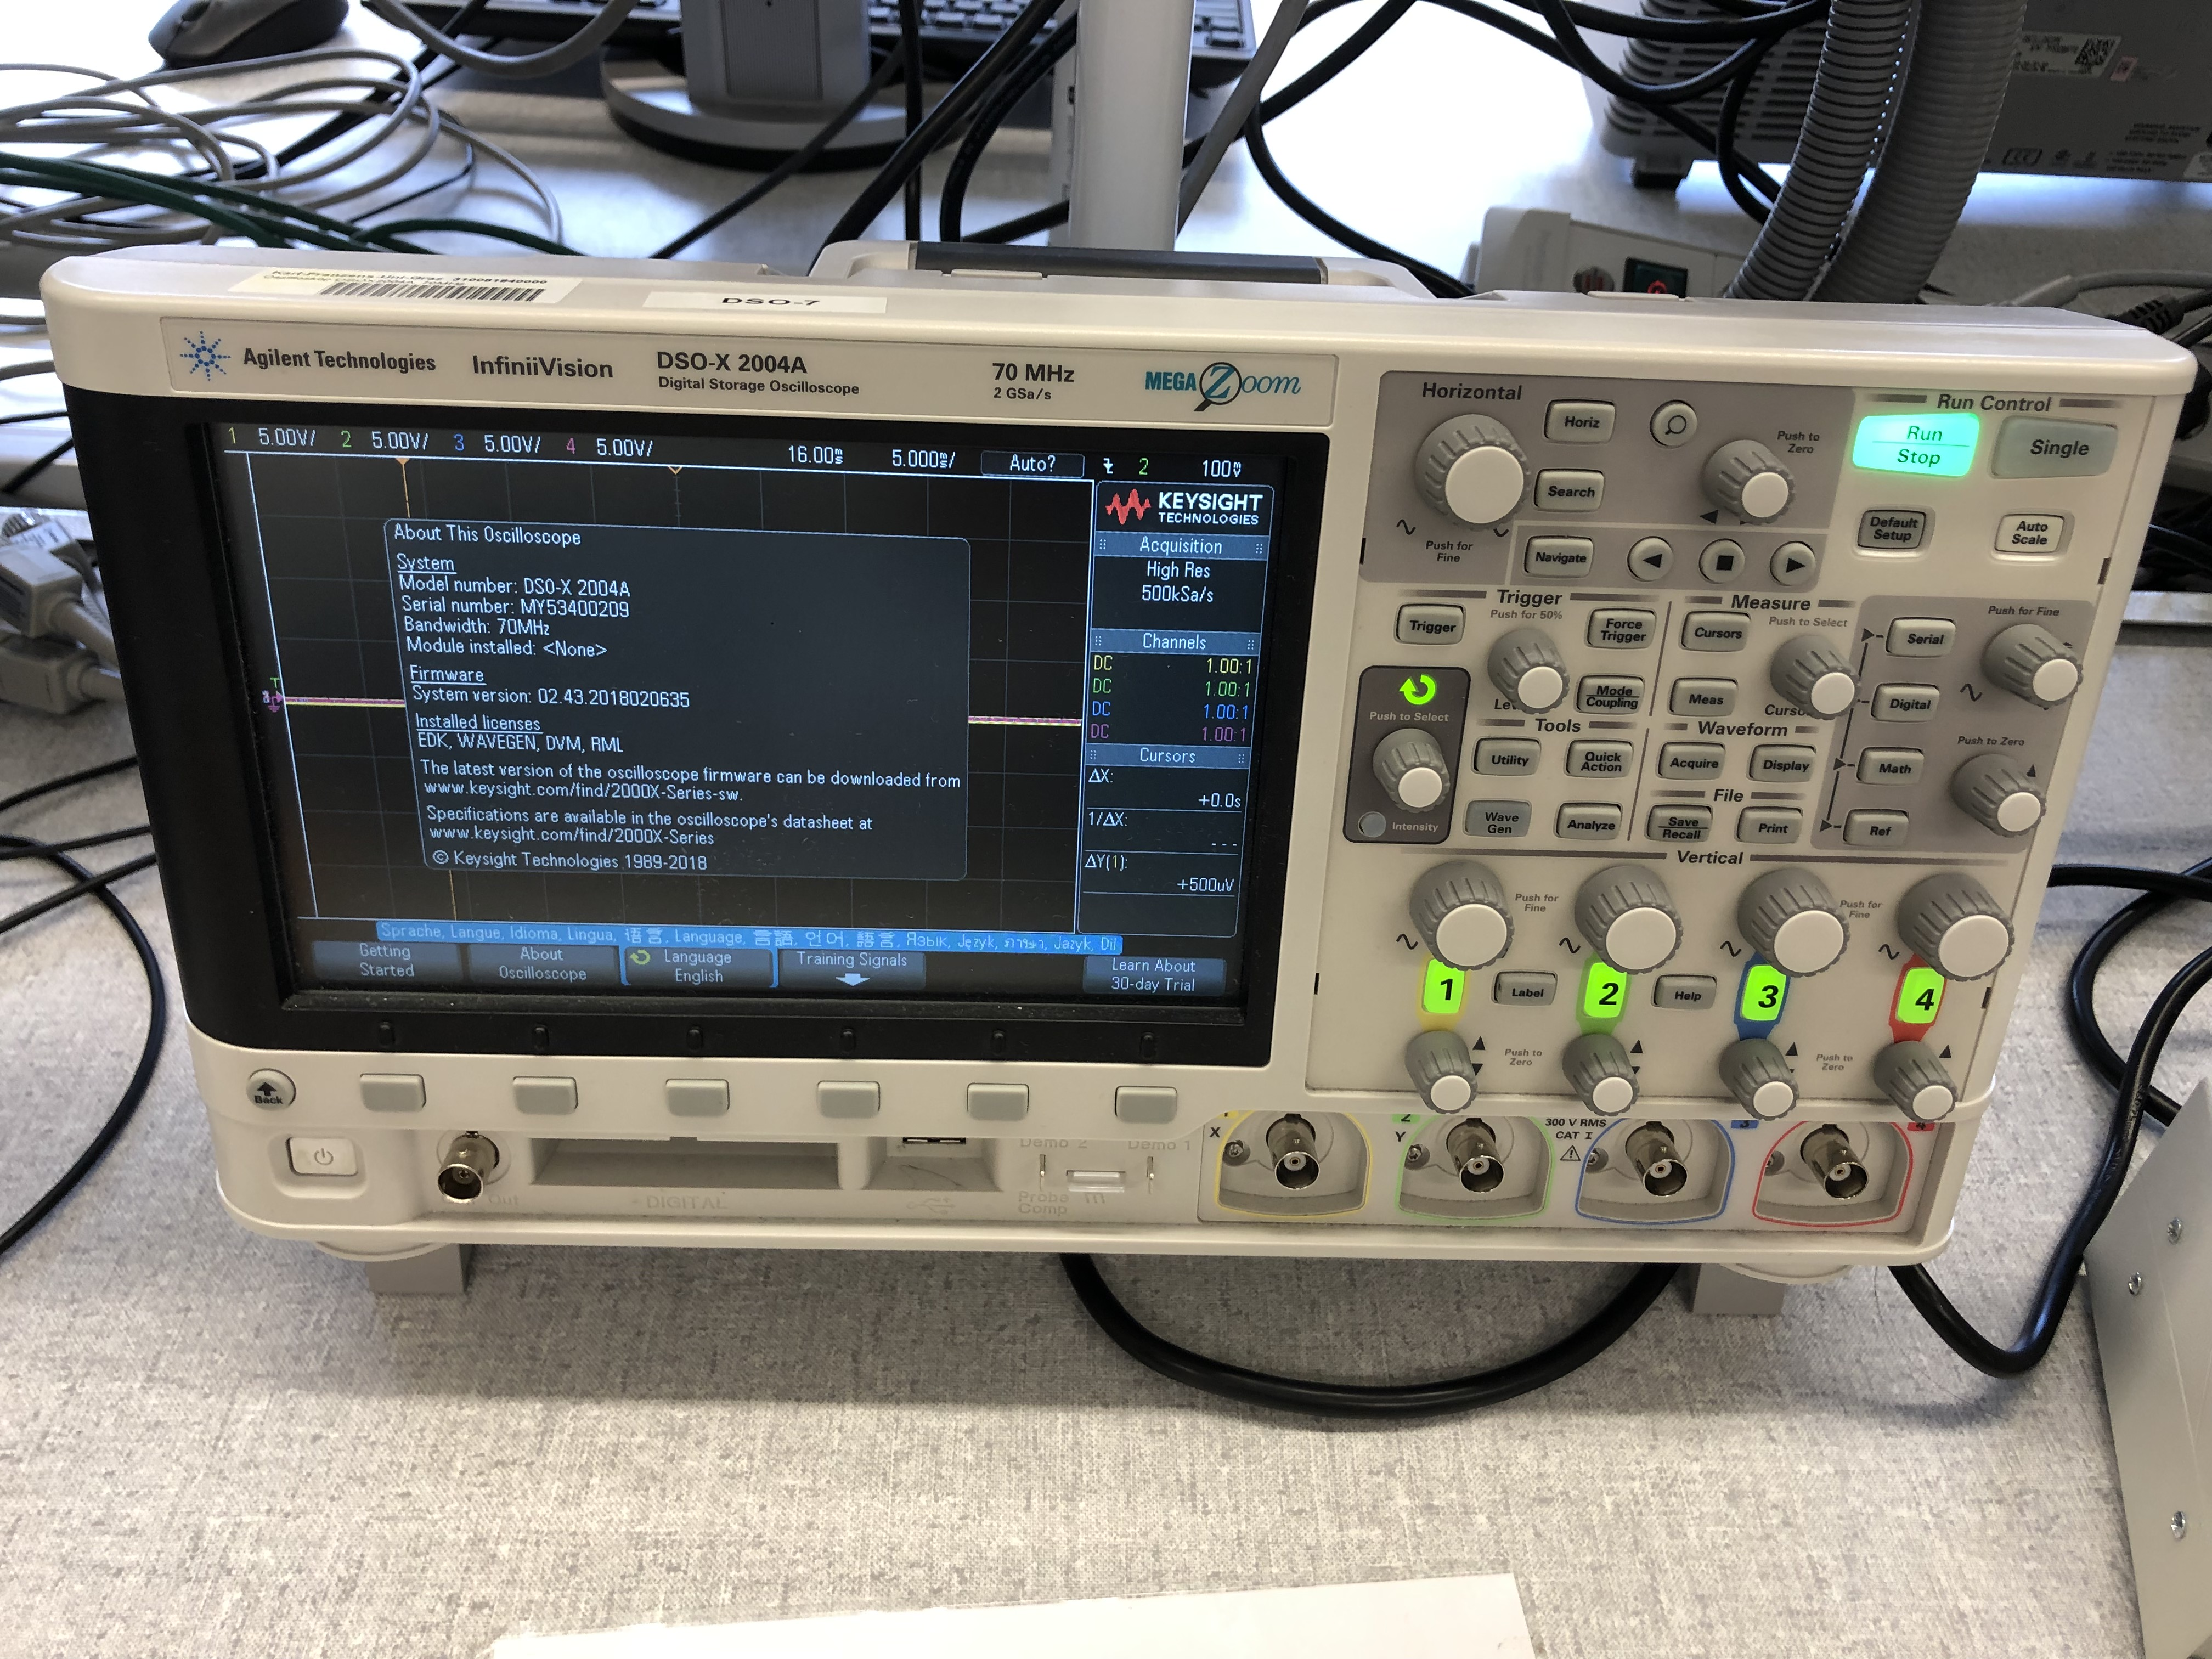
\includegraphics[width=\textwidth]{oszi}
		\captionof{figure}{Verwendetes Oszilloskop}
		\label{fig:oszi}
	\end{minipage}
	\vspace{1em}
\end{minipage}

Zusätzlich wurden ein Transformator, siehe \autoref{fig:transf} und digitale Multimeter, siehe \autoref{fig:multi}, verwendet.

\vspace{2mm}

\begin{minipage}{\textwidth}
	\begin{minipage}[t]{0.5\textwidth}
		\centering
		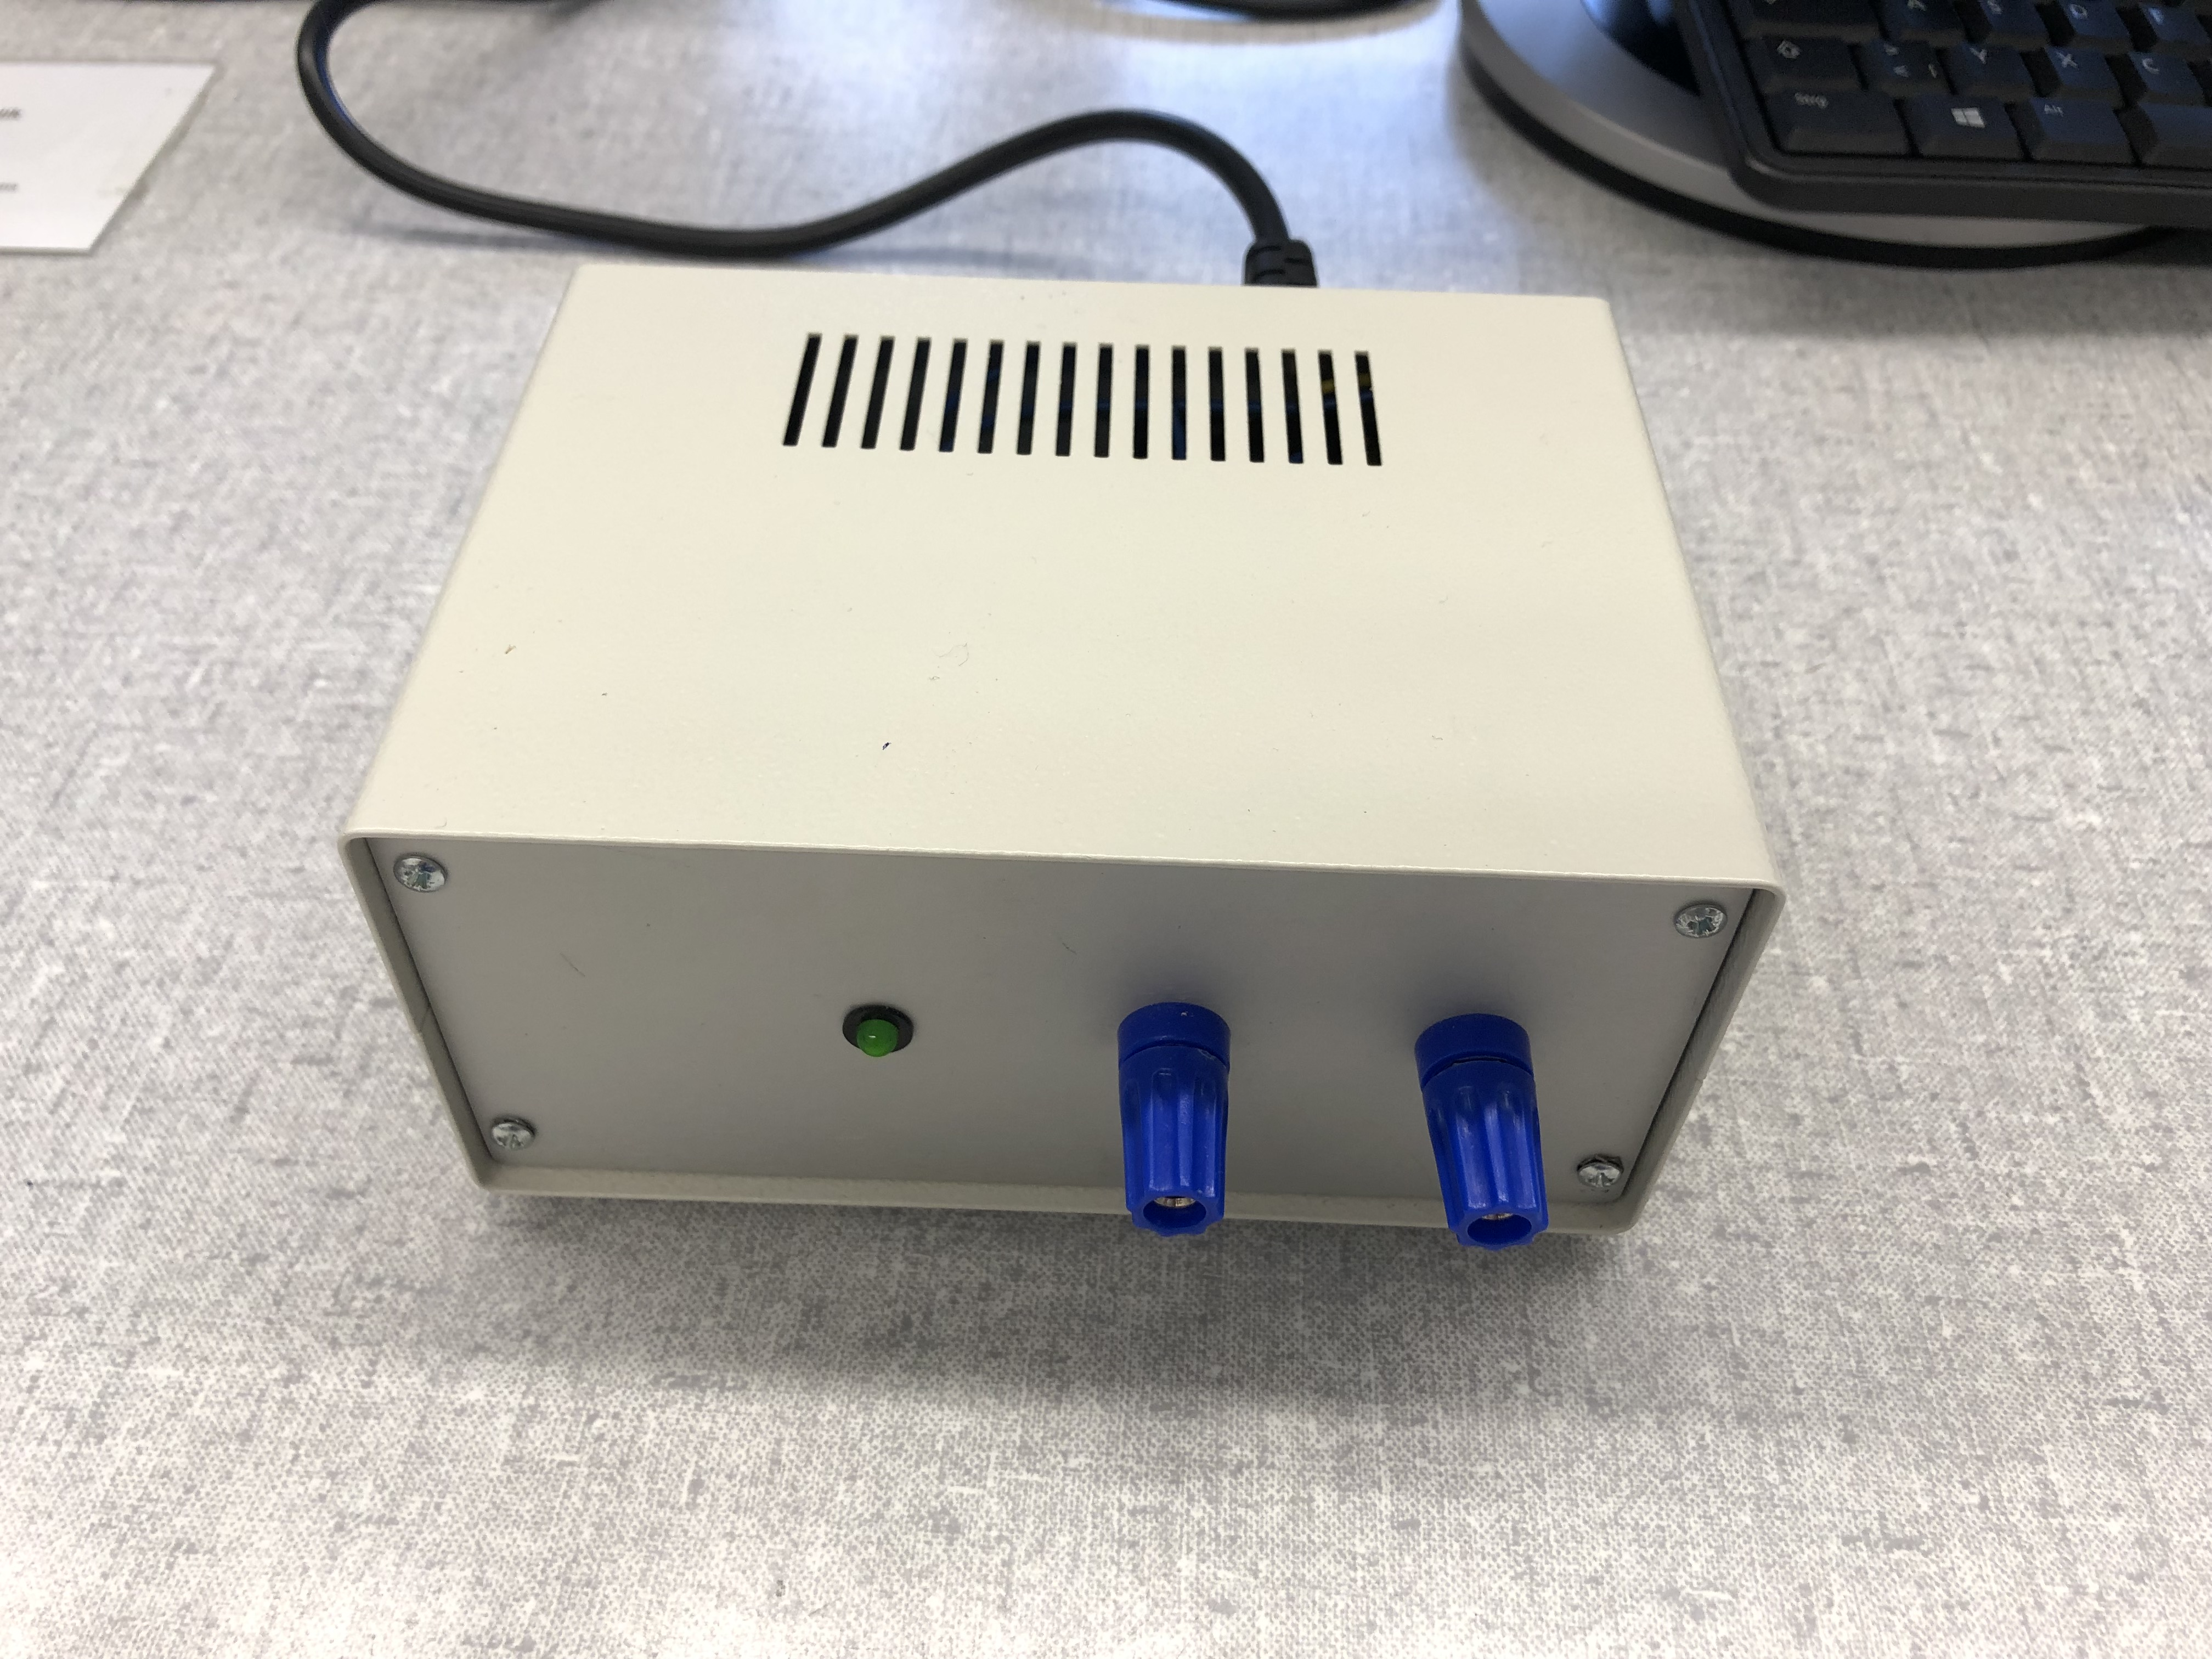
\includegraphics[width=\textwidth]{trafo}
		\captionbelowof{figure}{Verwendeter Transformator}
		\label{fig:transf}
	\end{minipage}
	\vspace{2mm}
	\begin{minipage}[t]{0.5\textwidth}
		\centering
		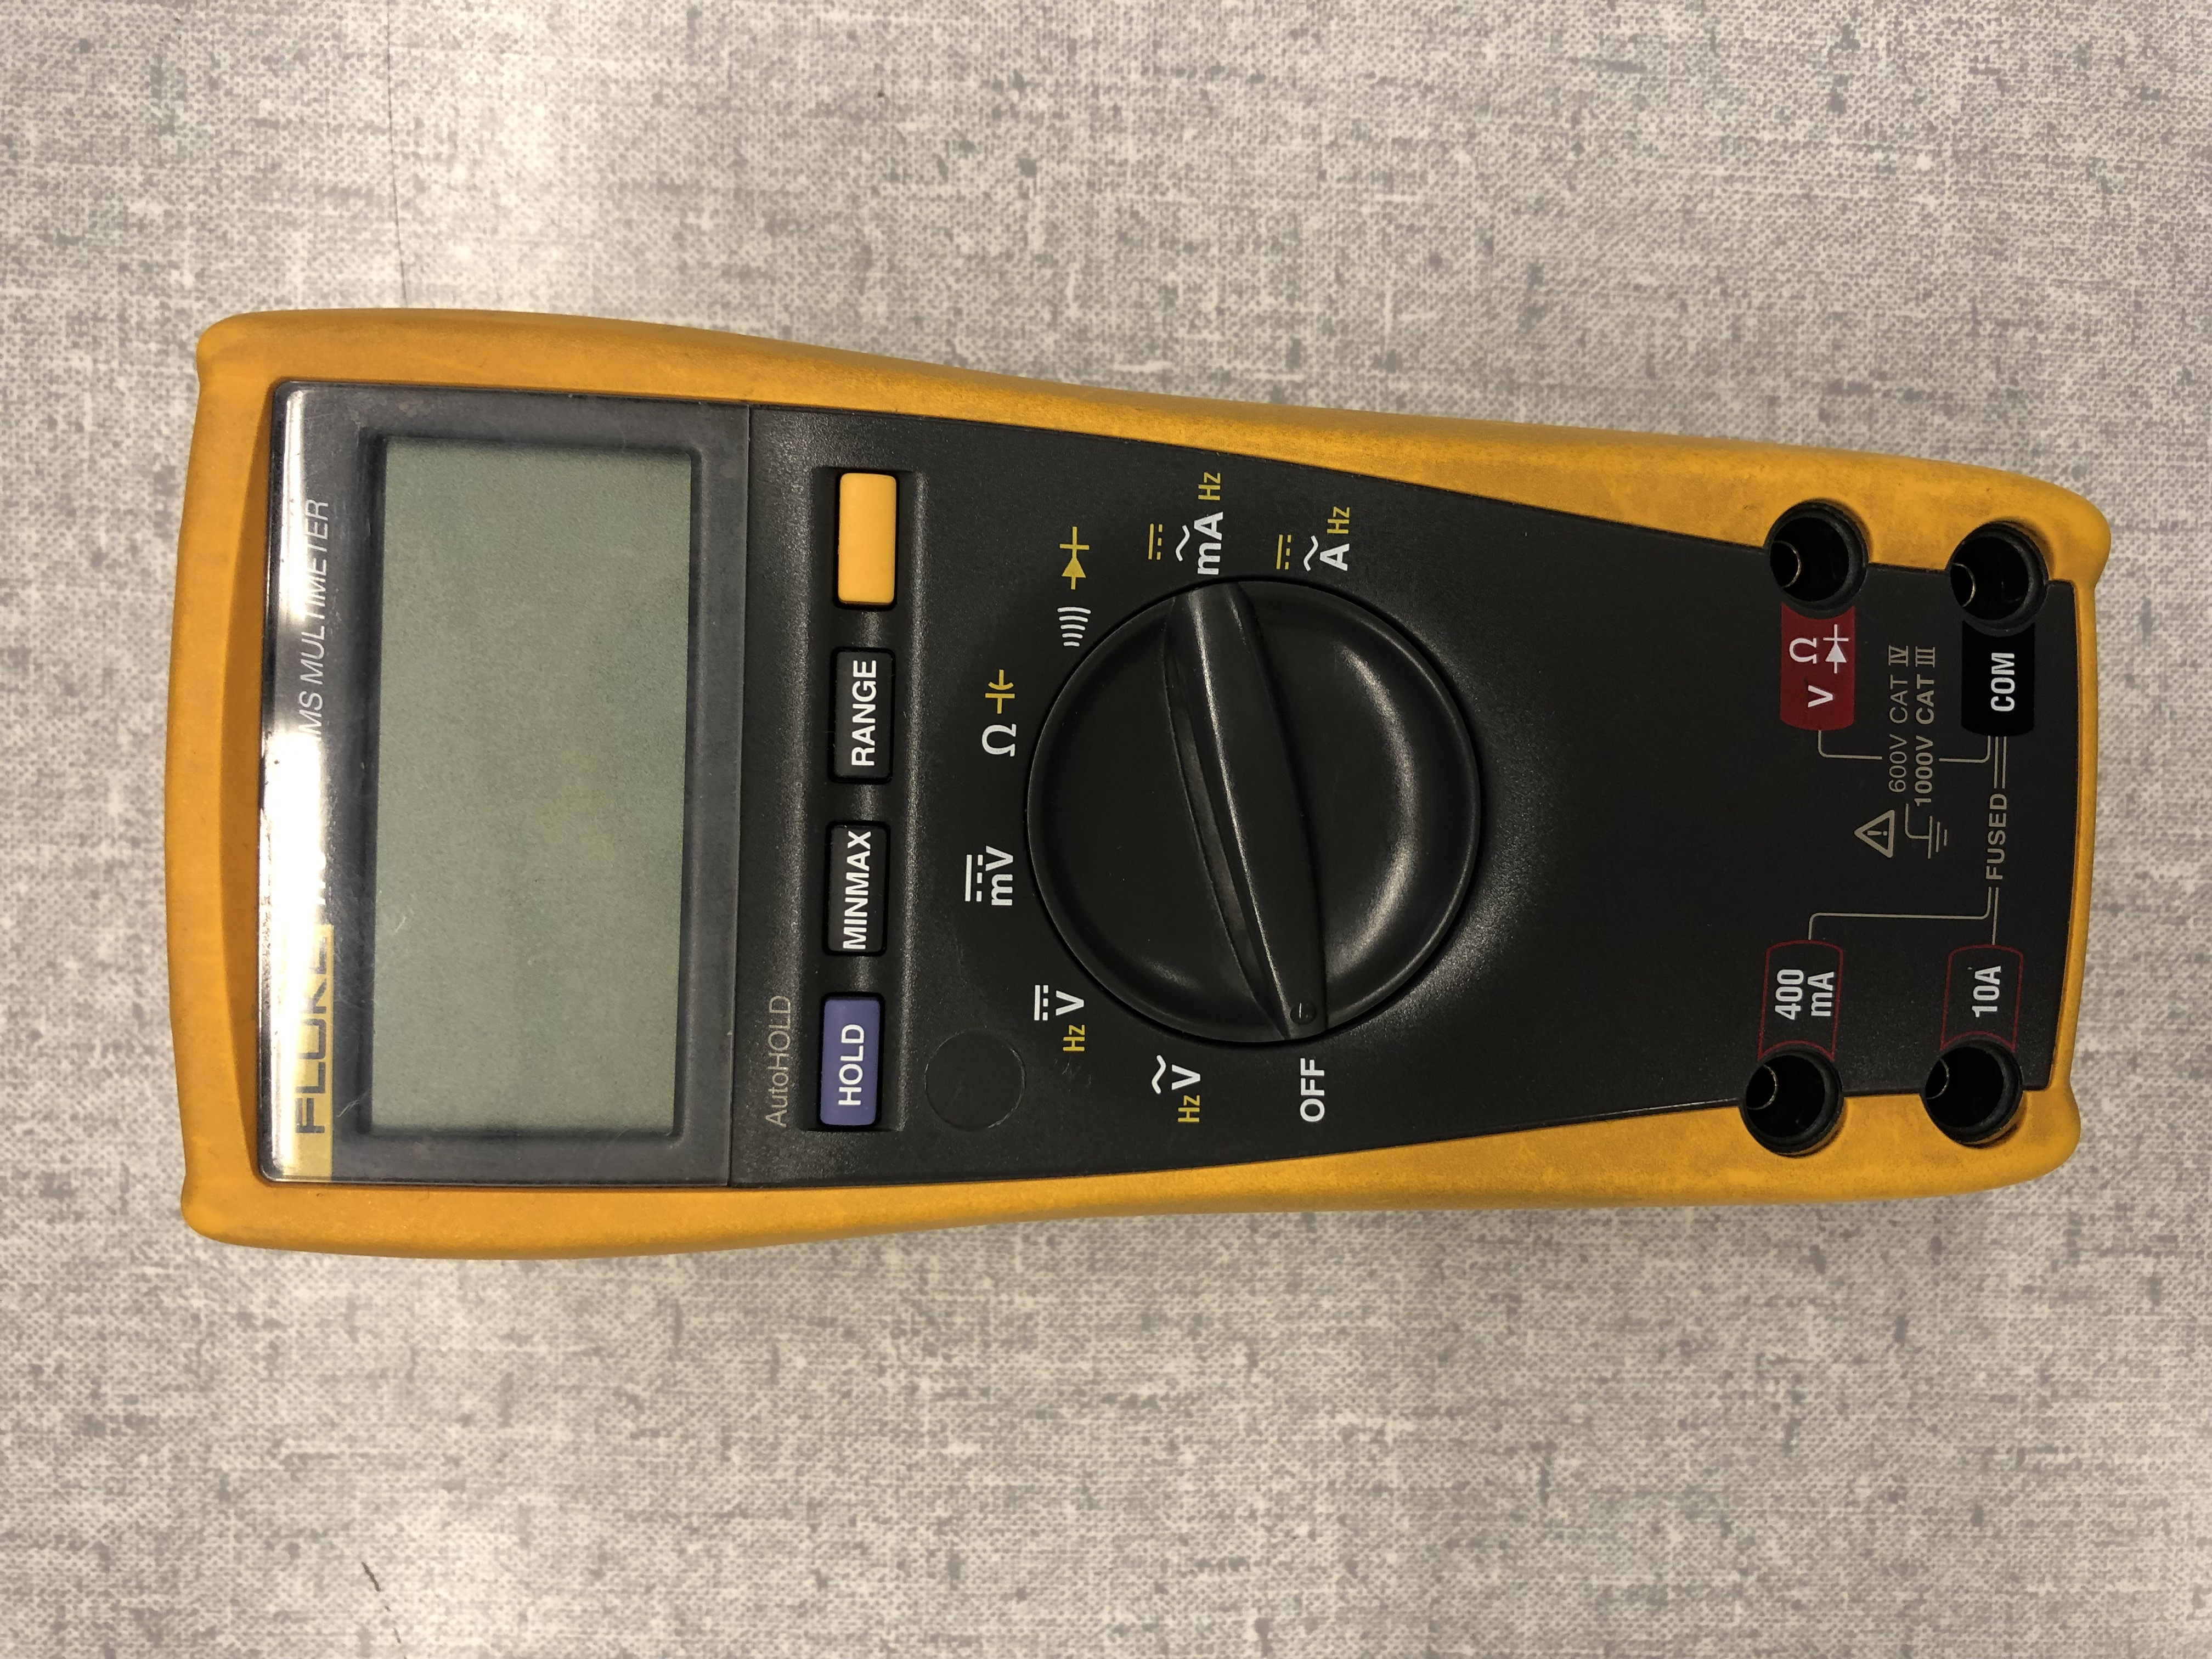
\includegraphics[angle = -90,width=\textwidth]{multi}
		\captionof{figure}{Verwendetes digitales Multimeter}
		\label{fig:multi}
	\end{minipage}
	\vspace{1em}
\end{minipage}

Um die entsprechenden Schaltungen zu verwirklichen wurden folgende Bauteile im Steckbrett verwendet, siehe \autoref{fig:steck}. Dabei handelt es sich um verschiedene Widerstände, die mithilfe des Multimeters aus \autoref{fig:multi} gemessen und die entsprechenden Werte bei der Abbildung in Blau gleich notiert wurden. Weiters sind 4 Gleichrichterdioden (1), eine  Zenerdiode (2), 2 Kondensatoren mit 100 $\mu$ Farad (3) und 2 Kondensatoren mit 10 $\mu$ Farad (4) sichtbar.

\vspace{2mm}

Um die Schaltungen zu verwirklichen wurden normale Kabel verwendet. Für den letzten Teil des Versuchs wurden zusätzlich noch Tastkabel, wie in \autoref{fig:tastkabel} sichtbar, verwendet, um das Oszilloskop entsprechend in die Schaltung zu integrieren.

\space{2mm}

\begin{minipage}{\textwidth}
	\begin{minipage}[t]{0.55\textwidth}
		\centering
		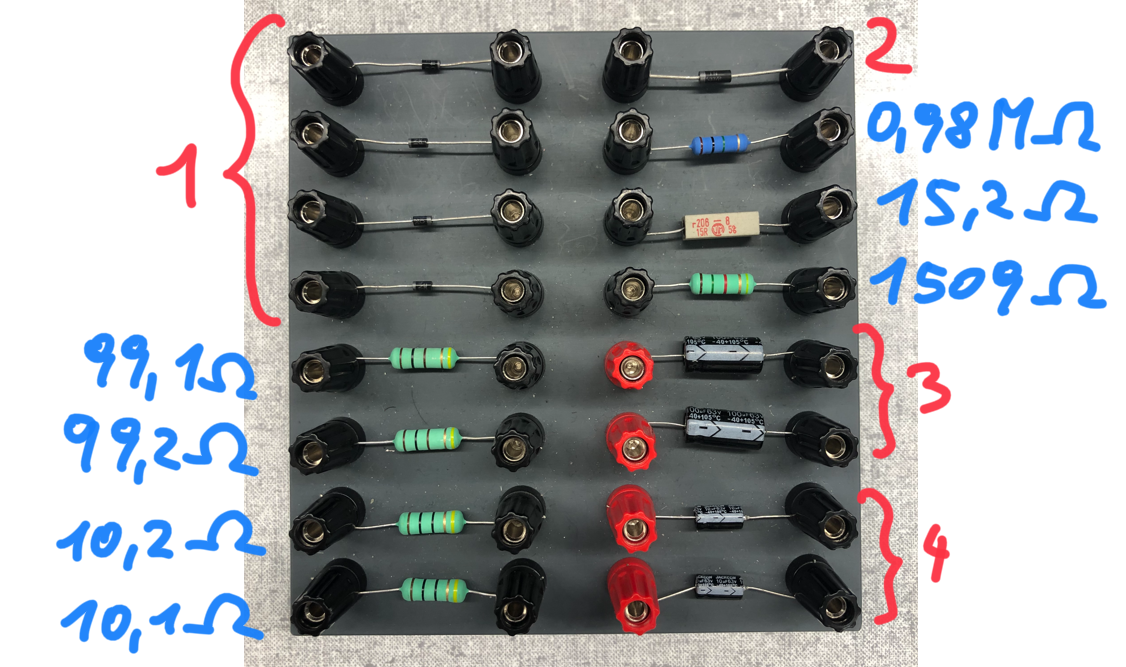
\includegraphics[width=\textwidth]{steck}
		\captionbelowof{figure}{Verwendete Bauteile im Steckbrett}
		\label{fig:steck}
	\end{minipage}
	\vspace{2mm}
	\begin{minipage}[t]{0.45\textwidth}
		\centering
		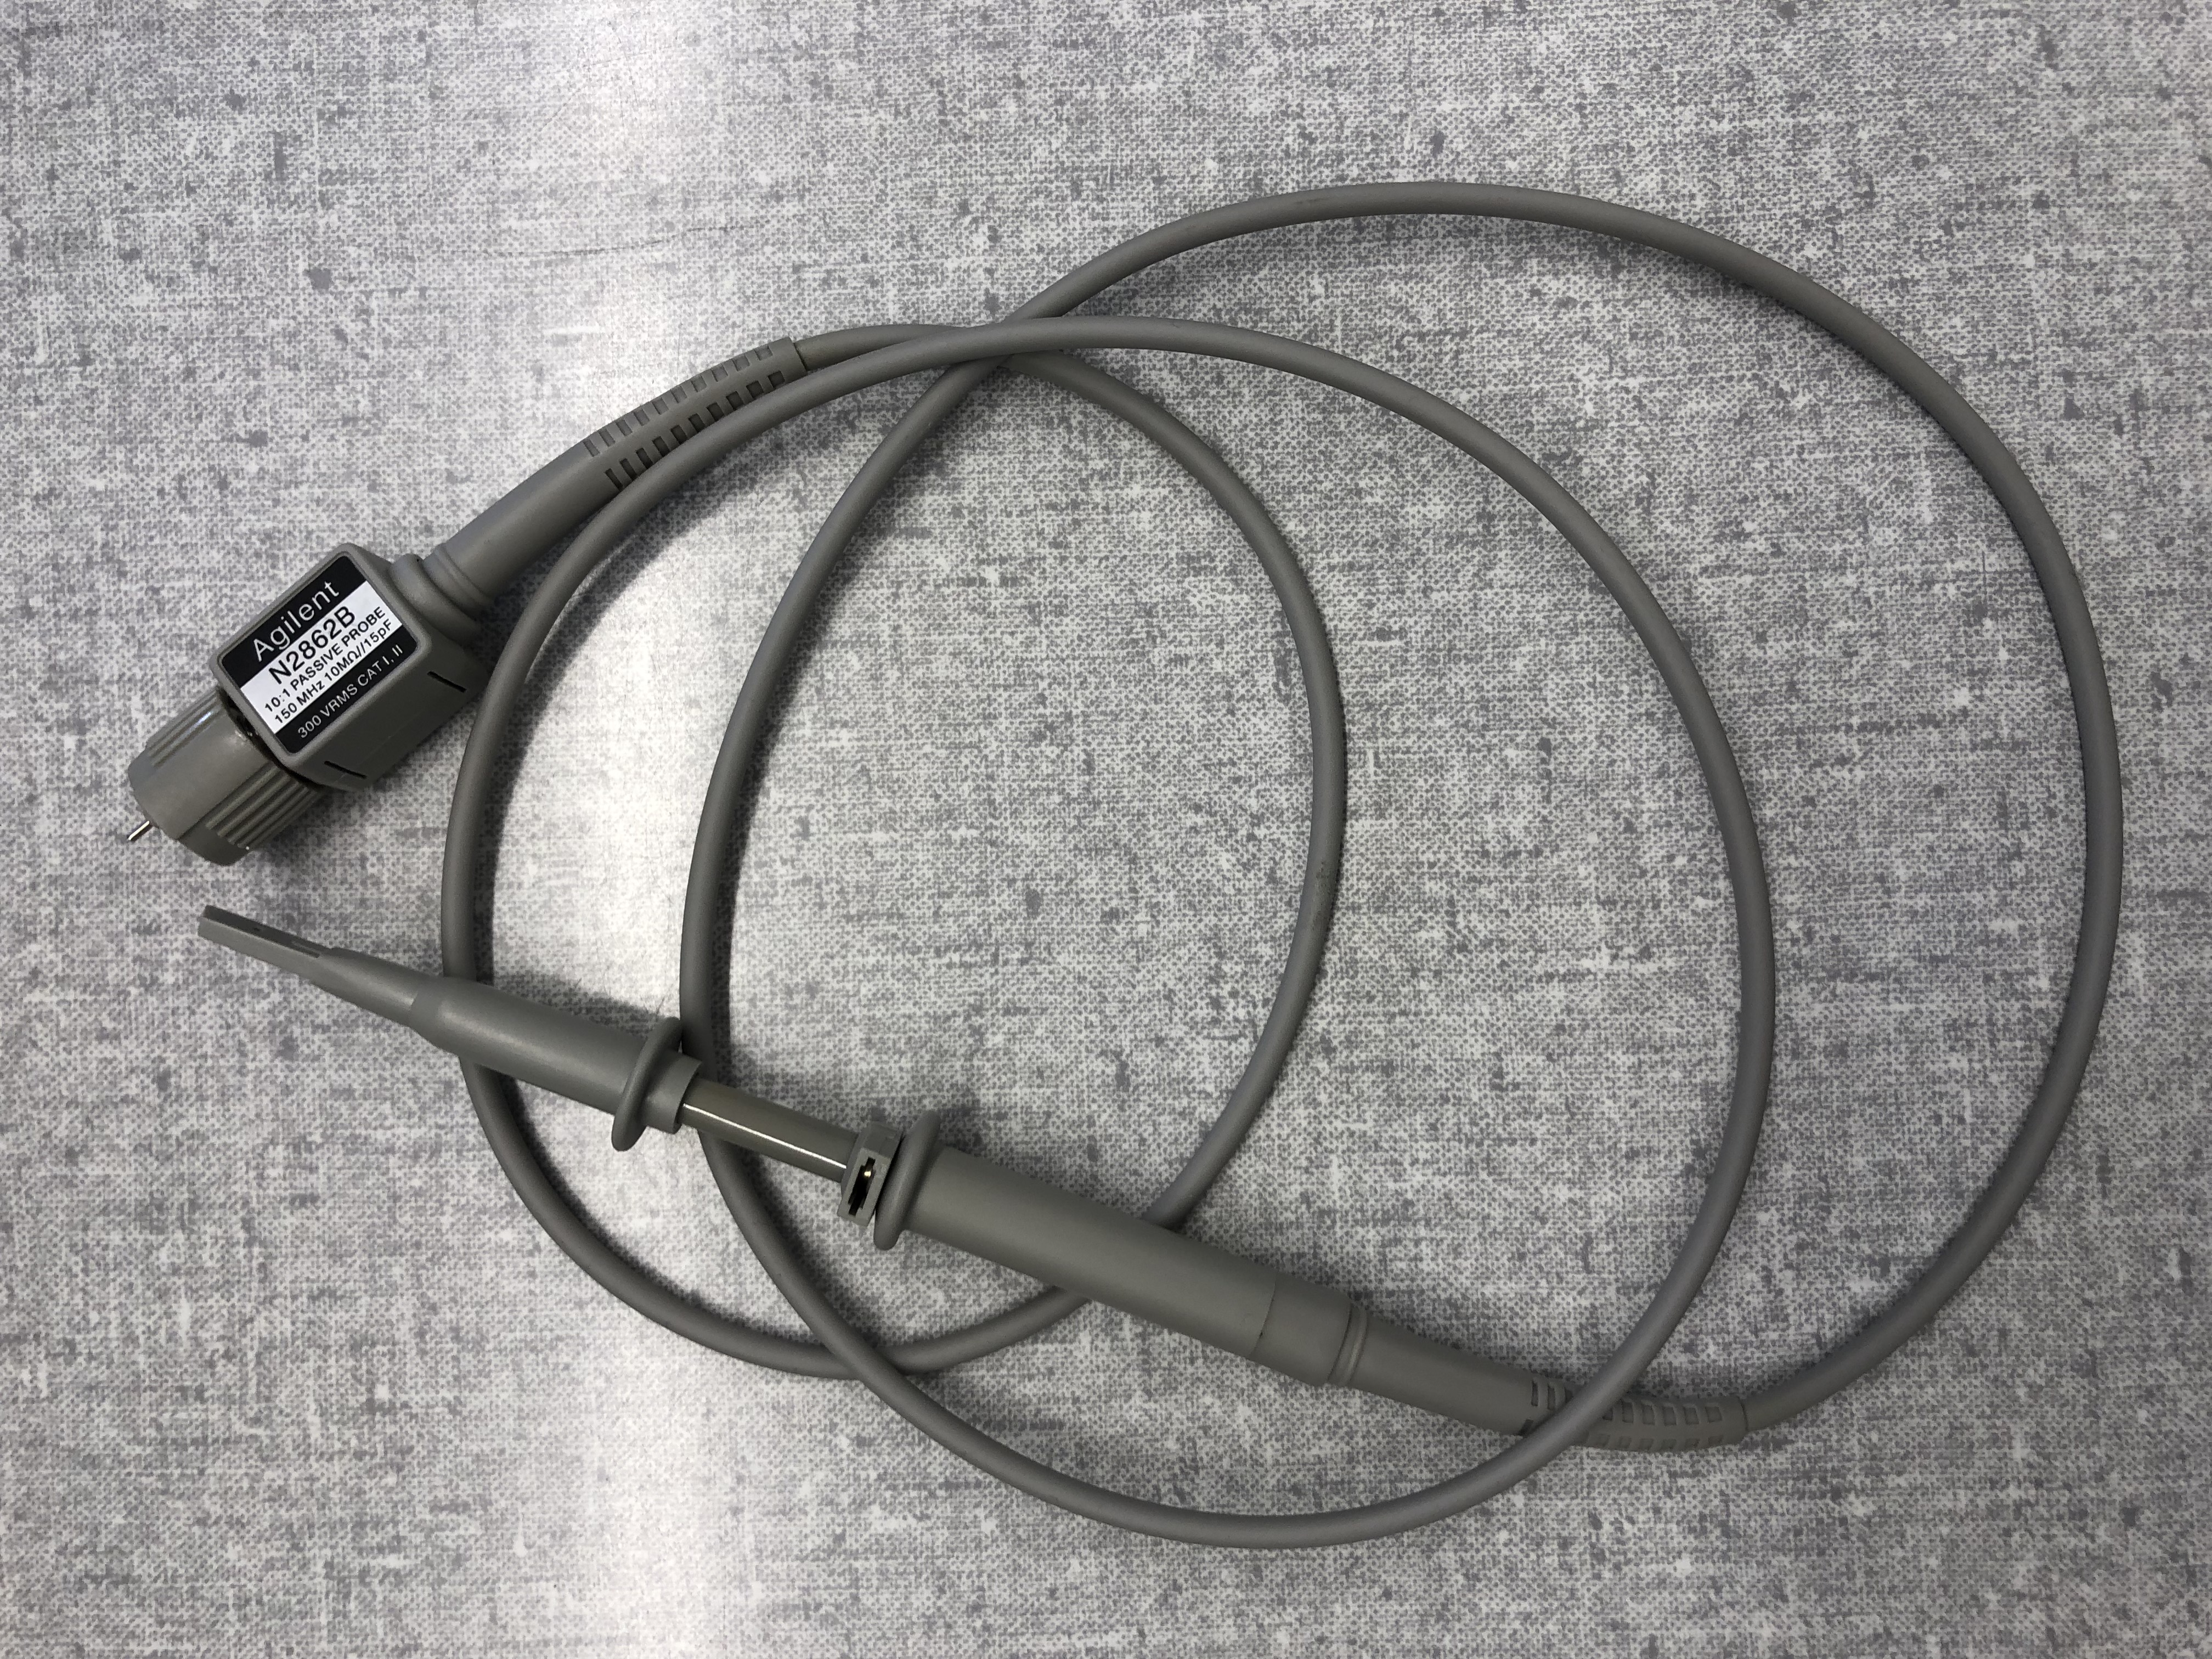
\includegraphics[width=\textwidth]{tastkabel}
		\captionof{figure}{Verwendete Tastkabel}
		\label{fig:tastkabel}
	\end{minipage}
	\vspace{1em}
\end{minipage}




\section{Geräteliste}

\noindent Für die Messungen wurden folgende Geräte verwendet:

\begin{center}
	\captionof{table}{Verwendete Geräte}
	\begin{tabular}{|c|c|c|c|c|} \hline
		\textbf{Gerät}      & \textbf{Typ}         & \textbf{Hersteller}  & \textbf{Seriennummer} \\ \hline
		Oszilloskop         & DSO-X 2004A          & Agilent Technologies & MY53400209            \\ \hline
		``Power Supply``    & HM8040-3             & Hameg Instruments    & PS-10                 \\ \hline
		2 Multimeter        & 175 True RMS         & Fluke                & AP-08 \& AP-13        \\ \hline
		Transformator       &                      &                      &                       \\ \hline
		Kabel               & 60 V DC 16 A         &                      &                       \\ \hline
		Tastkabel           & N2862B 300 VRMS CATI & Agilent              &                       \\ \hline
		Steckbrett          &                      &                      &                       \\ \hline
		Gleichrichterdioden & 1N4007               &                      &                       \\ \hline
		Zenerdioden         & 1N5337               &                      &                       \\ \hline
		2 Widerstände       & 100 $\Omega$         &                      &                       \\ \hline
		2 Widerstände       & 10 $\Omega$          &                      &                       \\ \hline
		Widerstand          & 1000000 $\Omega$     &                      &                       \\ \hline
		Widerstand          & 15 $\Omega$          &                      &                       \\ \hline
		Widerstand          & 1500 $\Omega$        &                      &                       \\ \hline
		2 Kondensatoren     & 100 $\mu$ Farad      &                      &                       \\ \hline
		2 Kondensatoren     & 10 $\mu$ Farad       &                      &                       \\ \hline
	\end{tabular}
	\label{tab:material}
\end{center}

\newpage

\section{Versuchsdurchführung \& Messergebnisse}\label{sec:Versuchsdurchführung}

Zunächst werden die genauen Werte der Widerstände mithilfe eines Multimeters gemessen. Die so erhaltenen Werte werden, der besseren Übersicht halber in Blau in \autoref{fig:steck} ergänzt.

\subsection{Ermittlung der Strom-Spannungscharakteriskik einer Gleichrichterdiode}

\subsubsection{in Durchlassrichtung}

Zunächst wird der Stromkreis nach folgenden Schaltplan in \autoref{fig:1a}
aufgebaut. Dabei ist vor allem zu beachten, dass die Diode richtig in den
Stromkreis geschlossen wird. Dies kann mit dem kleinen Diodenring an dessen
Rand überprüft werden.

\begin{center}
	\begin{minipage}[t]{0.7\textwidth}
		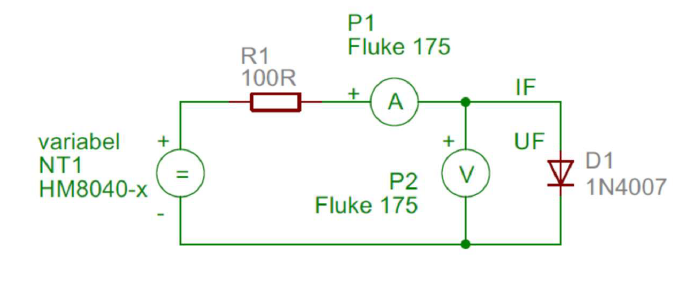
\includegraphics[width=\textwidth]{skizze_1a}
		\captionof{figure}{Skizze des Schaltplans, der für die erste Aufgabe benötigt wird \cite{halbleitervorlage}}
		\label{fig:1a}
	\end{minipage}
\end{center}

\noindent Der tatsächliche Aufbau ist in folgender \autoref{fig:aufbau1a} sichtbar.

\begin{center}
	\begin{minipage}[t]{0.7\textwidth}
		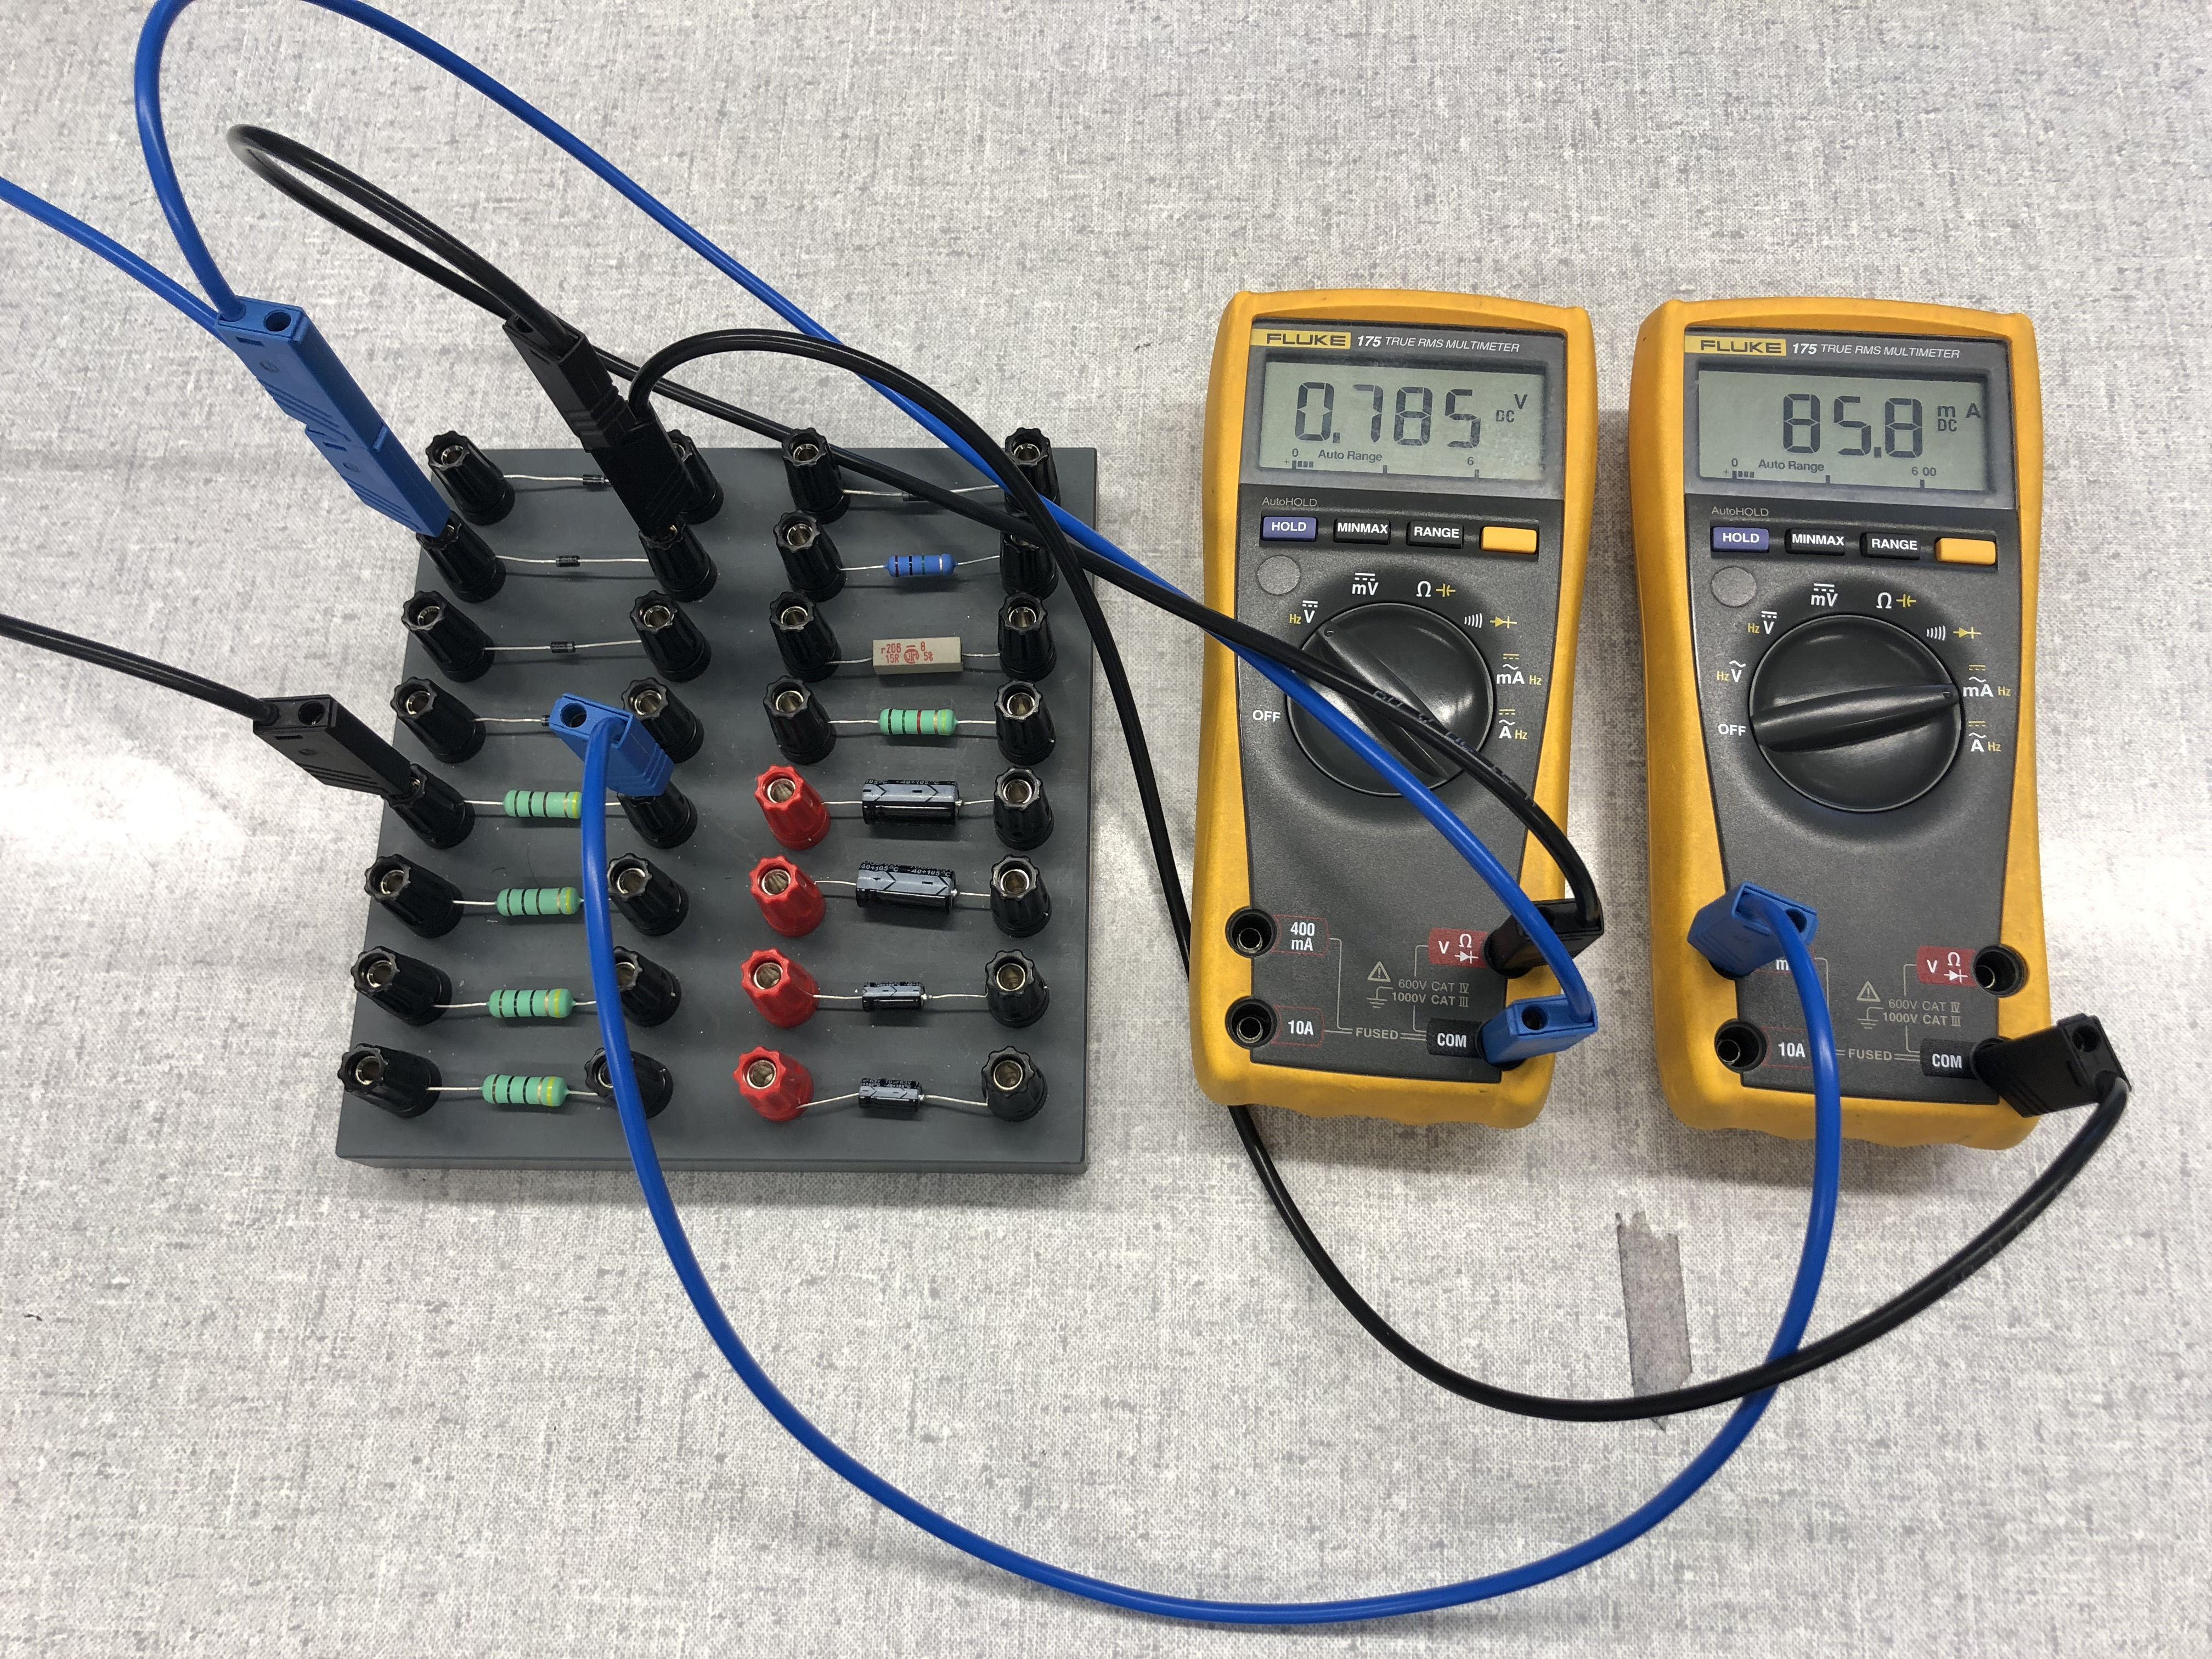
\includegraphics[width=\textwidth]{aufbau1a}
		\captionof{figure}{Versuchsaufbau für die Ermittlung der Strom-Spannungscharakteriskik einer Gleichrichterdiode in Durchlassrichtung}
		\label{fig:aufbau1a}
	\end{minipage}
\end{center}

Der Ausgang der Signalquelle war dabei durch das ``Hameg Power Supply`` gegeben. Um die Kennlinie aufzunehmen, wurden 14 Datenpunkte aufgezeichnet, die in folgender \autoref{tab:1a} aufgelistet sind. Zunächst wurde dabei die Spannung reguliert, bis diese bei einem aufgezeichneten Wert von \SI{0.70(5)}{mV} am ``Power Supply`` zunächst nicht mehr anwuchs. Dann wurde der Strom von einem Wert von \SI{8.0(5)}{mA} bis zu \SI{100.0(5)}{mA} erhöht und notiert. Die genauen Werte wurden dabei von den beiden Multimeter abgelesen.

\captionof{table}{Abgelesene Werte auf den Multimeter für die Spannung und die Stromstärke \\ $U_F$ \dots abgelesener Wert der Spannung in mV \\ $\Delta U_F$ \dots entsprechende Unsicherheit der Spannung in mV \\ $I_F$ \dots abgelesener Wert der Stromstärke in mA \\ $\Delta I_F$ \dots entsprechende Unsicherheit der Stromstärke in mA}
\begin{center}
	\begin{tabular}{lrrrrr}
		\toprule
		{}                         & {$U_F$} / mV & {$\Delta U_F$} / mV & {$I_F$} /mA & {$\Delta I_F$} /mA \\
		\midrule
		Regulation der Spannung    & 0.3          & 0.3                 & 0.0         & 0.2                \\
		                           & 127.4        & 0.4                 & 0.0         & 0.2                \\
		                           & 213.5        & 0.6                 & 0.0         & 0.2                \\
		                           & 376.2        & 0.8                 & 0.0         & 0.2                \\
		                           & 499.6        & 1.0                 & 0.0         & 0.3                \\
		                           & 545.8        & 1.1                 & 0.3         & 0.3                \\
		                           & 596.1        & 1.1                 & 1.0         & 0.3                \\
		                           & 614.5        & 1.2                 & 1.5         & 0.3                \\
		\midrule
		Regulation der Stromstärke & 707          & 4                   & 11.3        & 0.4                \\
		                           & 706          & 4                   & 12.6        & 0.4                \\
		                           & 747          & 4                   & 30.4        & 0.6                \\
		                           & 766          & 4                   & 52.2        & 0.8                \\
		                           & 782          & 4                   & 77.3        & 1.0                \\
		                           & 793          & 4                   & 102.2       & 1.3                \\
		\bottomrule
	\end{tabular}
	\label{tab:1a}
\end{center}

\newpage

\subsubsection{in Sperrrichtung}

Nun wird der Stromkreis nach folgenden Schaltplan in \autoref{fig:1b} aufgebaut. Weil das ``TTi 1604`` Gerät nicht zur Verfügung stand, wurde auch hier wieder ein zweites Multimeter zur Bestimmung der Spannung verwendet.

\begin{center}
	\begin{minipage}[t]{0.8\textwidth}
		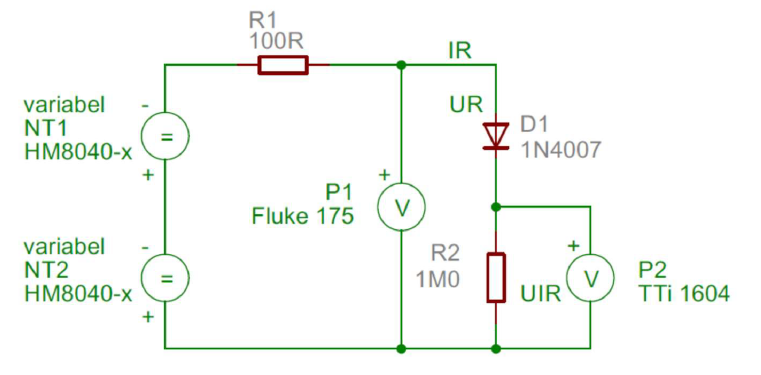
\includegraphics[width=\textwidth]{skizze_1b}
		\captionof{figure}{Skizze des Schaltplans, der für die Ermittlung der
			Strom-Spannungscharakteriskik einer Gleichrichterdiode in Sperrrichtung
			benötigt wird \cite{halbleitervorlage}}
		\label{fig:1b}
	\end{minipage}
\end{center}

\noindent Der tatsächliche Aufbau ist in folgender \autoref{fig:aufbau1b} sichtbar.

\begin{center}
	\begin{minipage}[t]{0.7\textwidth}
		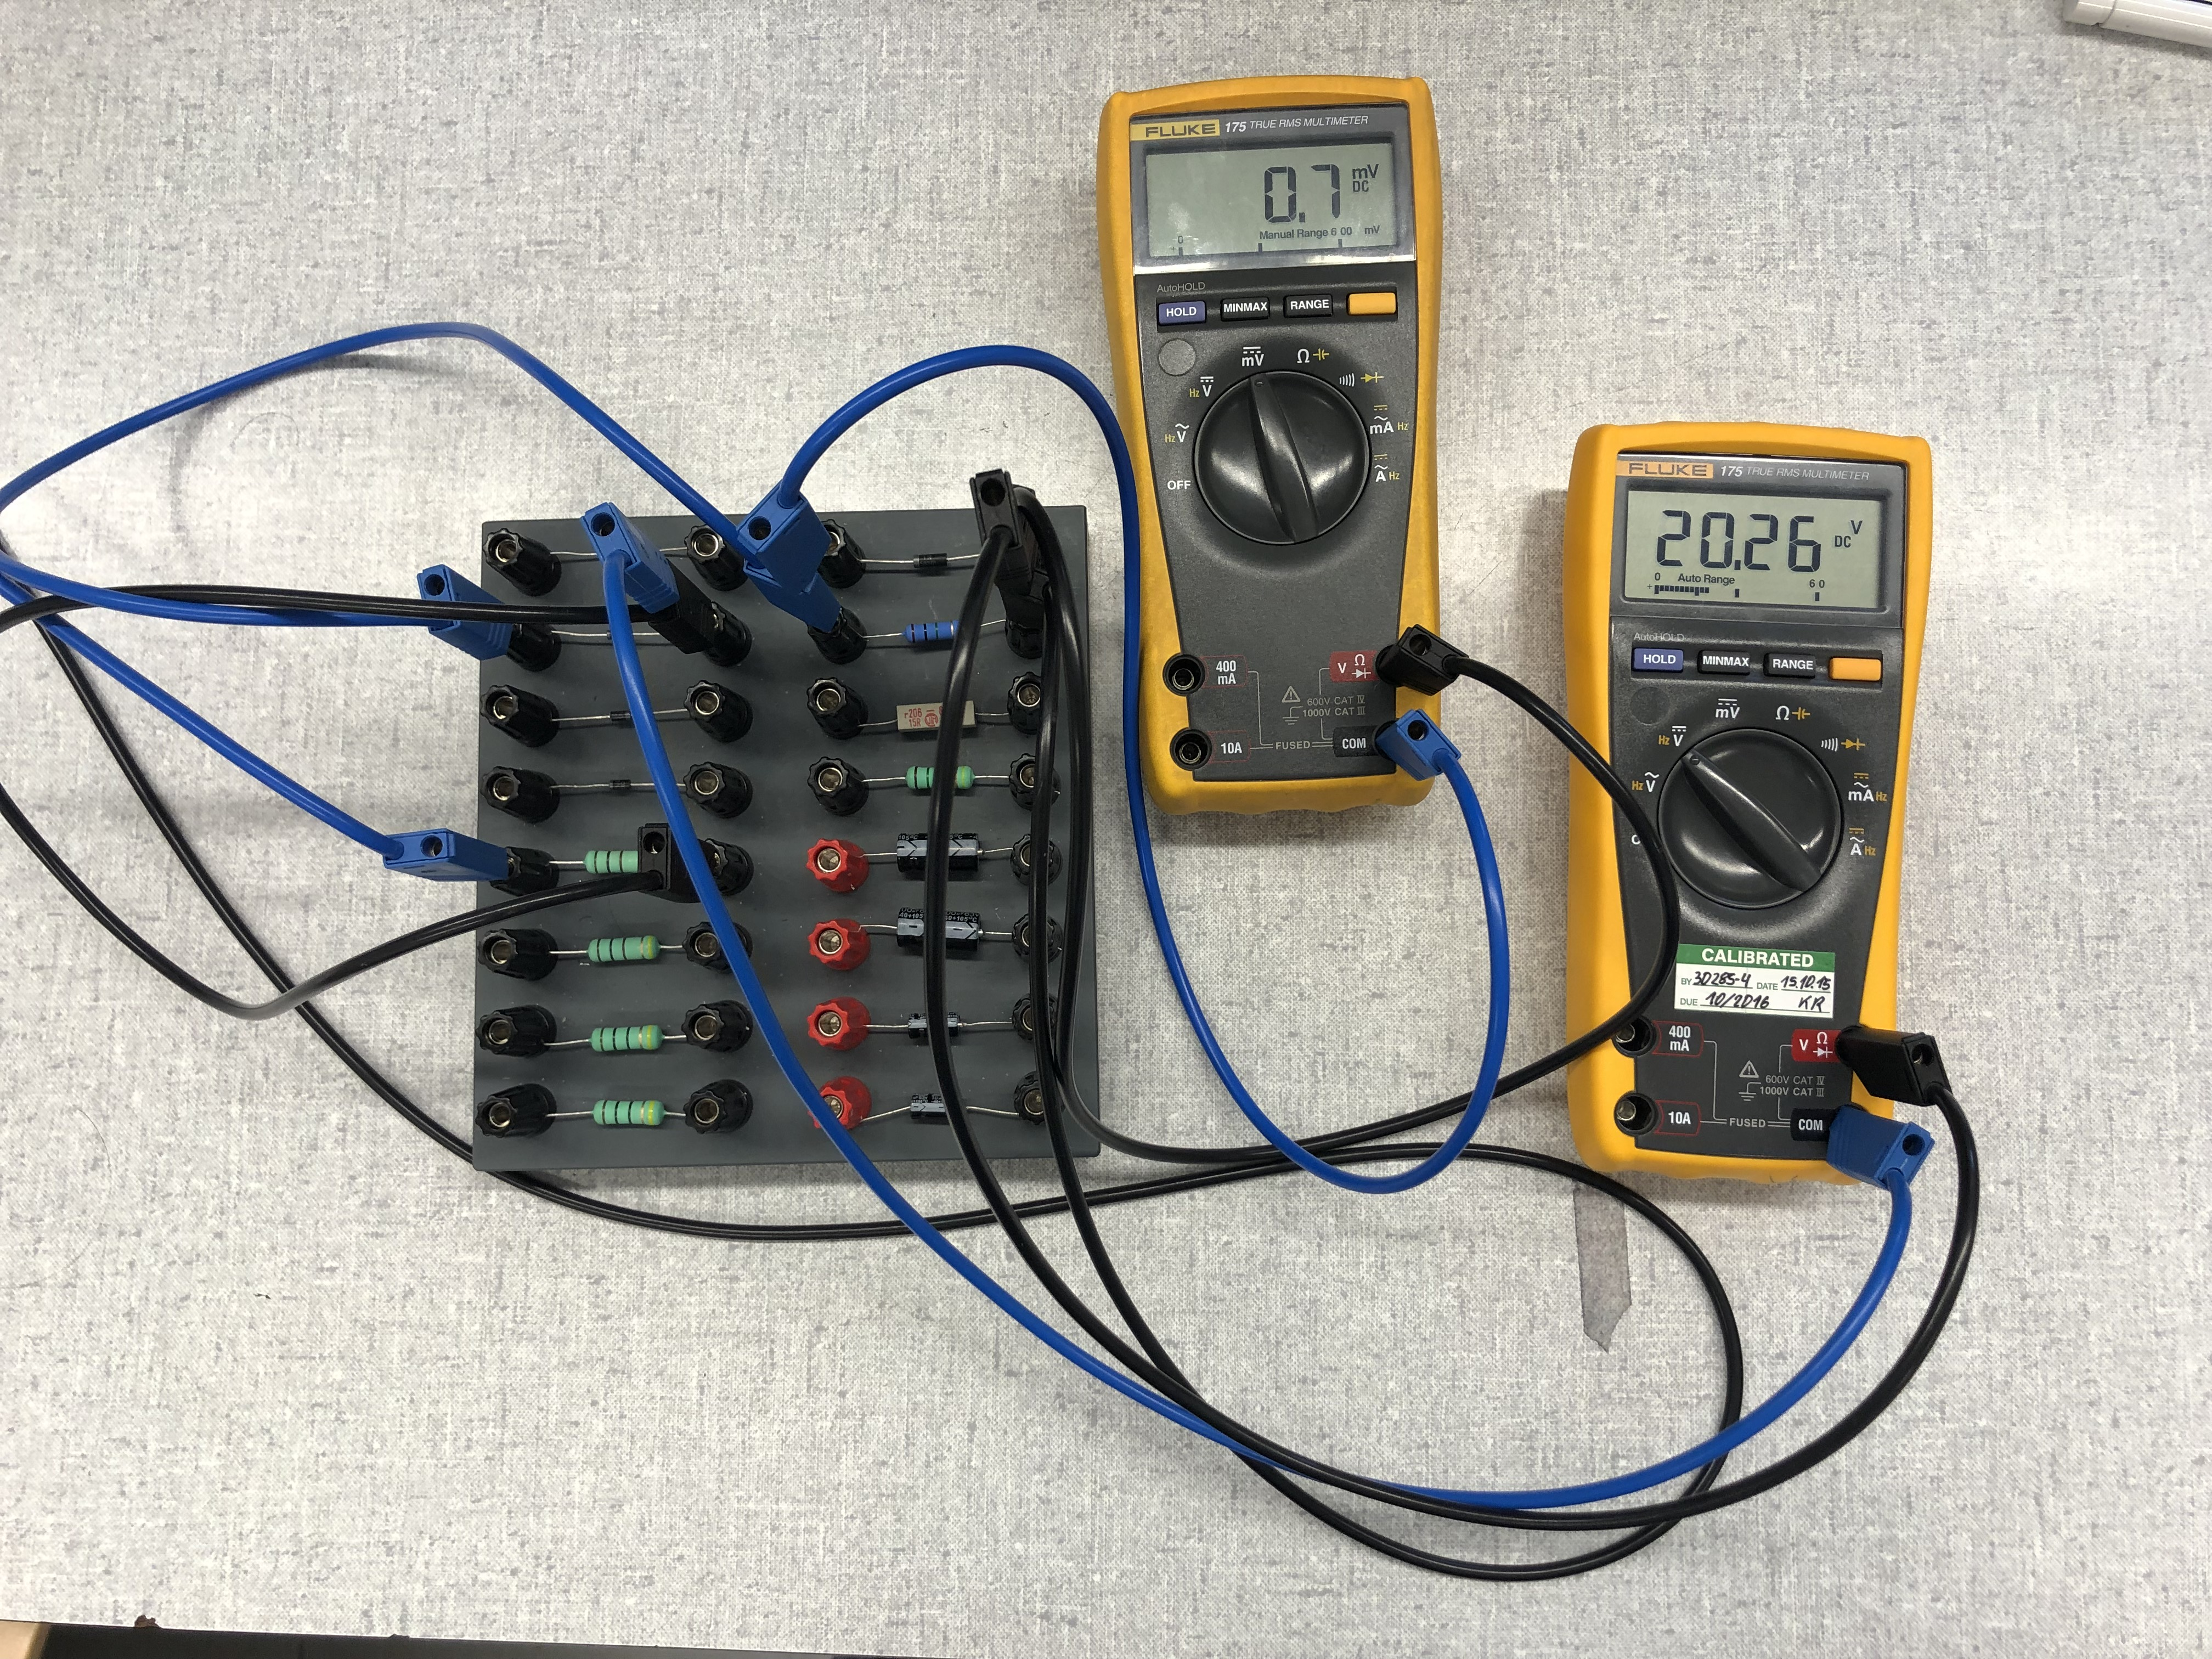
\includegraphics[width=\textwidth]{aufbau1b}
		\captionof{figure}{Versuchsaufbau für die Ermittlung der Strom-Spannungscharakteriskik einer Gleichrichterdiode in Sperrrichtung}
		\label{fig:aufbau1b}
	\end{minipage}
\end{center}

Als Signalausgang dient, wie auch zuvor, das ``Hameg Power Supply``. Die Ausgangsspannung wird dabei im Bereich von \SI{0.0(5)}{V} bis \SI{40.0(5)}{V} variiert und die genauen Werte wieder an den Multimeter abgelesen , was in \autoref{tab:1b} sichtbar ist. Der Sperrstrom $I_{Sperr}$ errechnet sich dabei als $\frac{U_{IR}}{R}$ und wird der besseren Übersicht halber ebenfalls schon dieser \autoref{tab:1b} beigefügt.


\captionof{table}{Abgelesene Werte auf den Multimeter für die beiden Spannungen \\ $U_R$ \dots abgelesener Wert der Gesamtspannung in V \\ $\Delta U_R$ \dots entsprechende Unsicherheit der Gesamtspannung in V \\ $U_{IR}$ \dots abgelesener Wert der Spannung am Widerstand in V \\ $\Delta U_{IR}$ \dots entsprechende Unsicherheit der Spannung am Widerstand in V \\ $I_{Sperr}$ \dots errechneter Wert des Sperrstroms in A \\ $\Delta I_{Sperr}$ \dots entsprechende Unsicherheit des Sperrstroms in A}
\begin{center}
	\begin{tabular}{lSSSSSS}
		\toprule
		{} & {$U_{R}$} & {$\Delta U_R$} & {$U_{IR}$} & {$\Delta U_{IR}$} & {$I_{Sperr}$} & {$\Delta I_{Sperr}$} \\
		\midrule
		0  & -0.0017   & 0.0003         & 0.0        & 0.03              & -0.000000e+00 & 4e-08                \\
		1  & -5.127    & 0.010          & 0.4        & 0.04              & -4.1e-07      & 4e-08                \\
		2  & -10.06    & 0.04           & 0.5        & 0.04              & -5.1e-07      & 4e-08                \\
		3  & -15.07    & 0.05           & 0.6        & 0.04              & -6.1e-07      & 4e-08                \\
		4  & -20.17    & 0.06           & 0.7        & 0.04              & -7.1e-07      & 4e-08                \\
		5  & -25.08    & 0.06           & 0.8        & 0.04              & -8.1e-07      & 4e-08                \\
		6  & -30.08    & 0.07           & 0.9        & 0.04              & -9.2e-07      & 4e-08                \\
		7  & -35.13    & 0.08           & 0.9        & 0.04              & -9.2e-07      & 4e-08                \\
		8  & -40.05    & 0.09           & 1.0        & 0.04              & -1.02e-06     & 4e-08                \\
		\bottomrule
	\end{tabular}
	\label{tab:1b}
\end{center}

\vspace{2mm}

\subsection{Ermittlung der Strom-Spannungscharakteriskik einer Zenerdiode}

Um die Strom-Spannungscharakteriskik einer Zenerdiode bestimmen zu können, wird der Stromkreis nach folgenden Schaltplan in \autoref{fig:2} aufgebaut.

\begin{center}
	\begin{minipage}[t]{0.8\textwidth}
		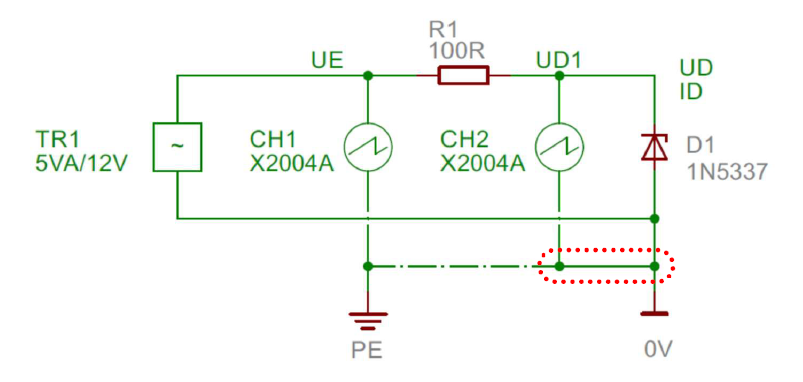
\includegraphics[width=\textwidth]{skizze_2}
		\captionof{figure}{Skizze des Schaltplans, der für die Ermittlung der
			Strom-Spannungscharakteriskik einer Zenerdiode benötigt wird
			\cite{halbleitervorlage}}
		\label{fig:2}
	\end{minipage}
\end{center}

\noindent Der tatsächliche Aufbau ist in folgender \autoref{fig:aufbau2} sichtbar. Weil leider keine passenden Adapterstücke für die Koaxialanschlüsse des Oszilloskops zu den vorhanden waren, wurden im Versuchsaufbau Koaxialkabel verwendet. Bei den Adapterstücken von den Bananenbuchsen zum Koaxialkabel
wird dabei immer nur der rote Steckplatz verwendet. Der schwarze dient dabei immer der Erdung und wird nur bei einem Stecker (Channel 1) angeschlossen.

\begin{center}
	\begin{minipage}[t]{0.5\textwidth}
		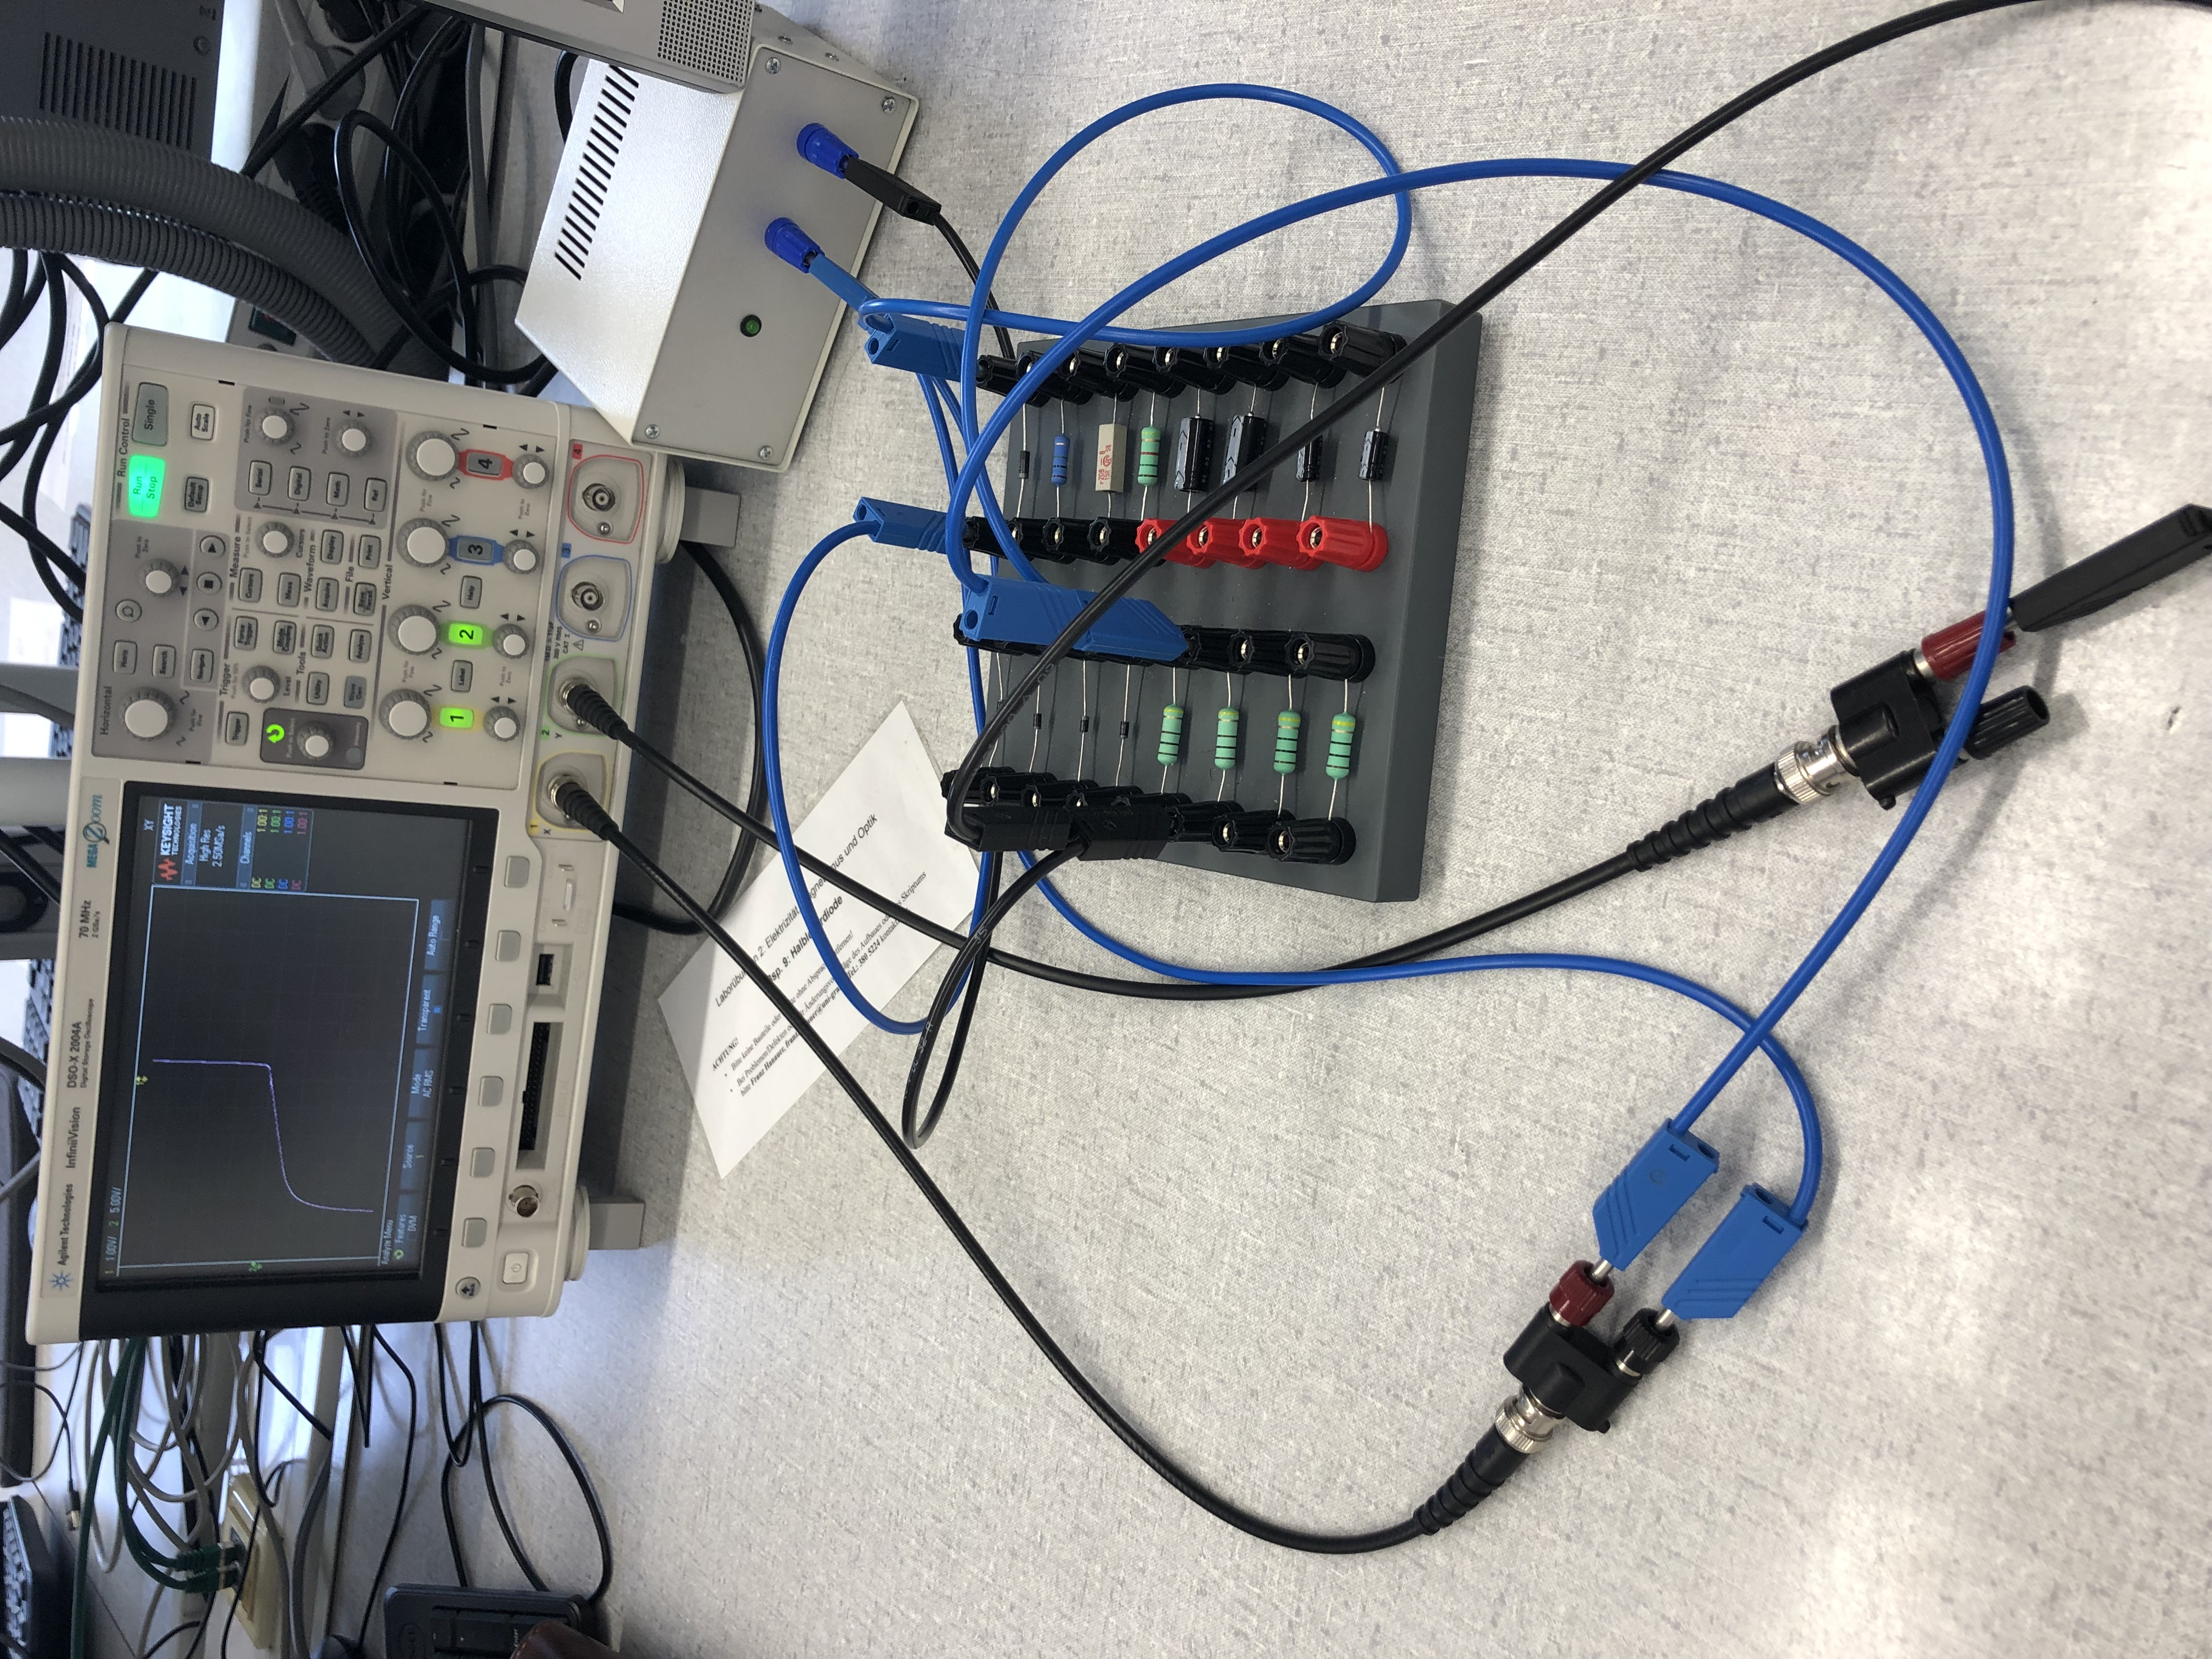
\includegraphics[angle=-90,width=\textwidth]{aufbau2}
		\captionof{figure}{Versuchsaufbau für die Ermittlung der Strom-Spannungscharakteriskik einer Zenerdiode}
		\label{fig:aufbau2}
	\end{minipage}
\end{center}

Um den Stromkreis nicht zu überlasten, wird am Oszilloskop nur ein ``single-shot`` mithilfe der gleichnamigen Einstellung aufgezeichnet. Der Trafo kann dadurch sofort wieder ausgeschaltet werden, während das, vom Oszilloskop aufgezeichnete Signal, ausgewertet wird. Dieses wird mithilfe eines USB-Sticks gespeichert und ist in folgender \autoref{fig:oszi2} sichtbar. Zusätzlich werden die so erhaltenen Daten auch als CSV-Datei gespeichert, um so mit dem entsprechenden Auswertungsprogrammen weiterverarbeitet werden zu können.

\begin{center}
	\begin{minipage}[t]{0.8\textwidth}
		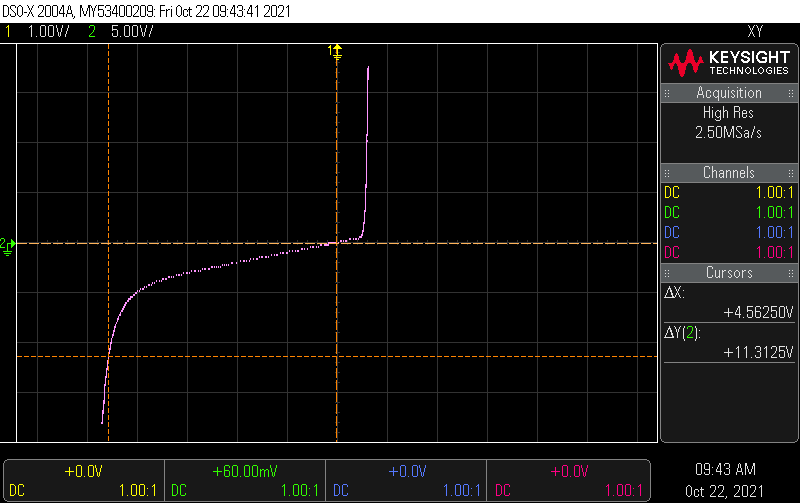
\includegraphics[width=\textwidth]{Halbleiter/scope_1}
		\captionof{figure}{Vom Oszilloskop aufgezeichnete Daten für die Kennlinie der Zenerdiode}
		\label{fig:oszi2}
	\end{minipage}
\end{center}


\subsection{Untersuchung der Strom- und Spannungsverläufe mit unterschiedlichen Glättungskondensatoren und Belastungswiderständen}

Um die Strom- und Spannungsverläufe mit unterschiedlichen Glättungskondensatoren und Belastungswiderständen bestimmen zu können, wird der Stromkreis nach folgenden Schaltplan in \autoref{fig:3} aufgebaut.

\begin{center}
	\begin{minipage}[t]{0.8\textwidth}
		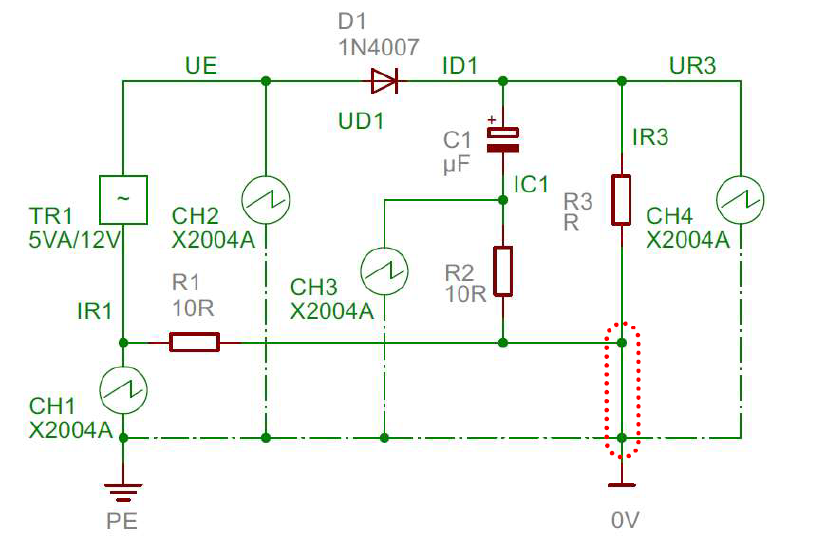
\includegraphics[width=\textwidth]{skizze_3}
		\captionof{figure}{Skizze des Schaltplans, der für die Ermittlung der
			Strom- und Spannungsverläufe mit unterschiedlichen Glättungskondensatoren
			und Belastungswiderständen benötigt wird \cite{halbleitervorlage}}
		\label{fig:3}
	\end{minipage}
\end{center}

\noindent Der tatsächliche Aufbau ist in folgender \autoref{fig:aufbau3} sichtbar. Die roten Kabel wurden dabei verwendet, um die unterschiedlichen Widerstände zu realisieren.

\begin{center}
	\begin{minipage}[t]{0.7\textwidth}
		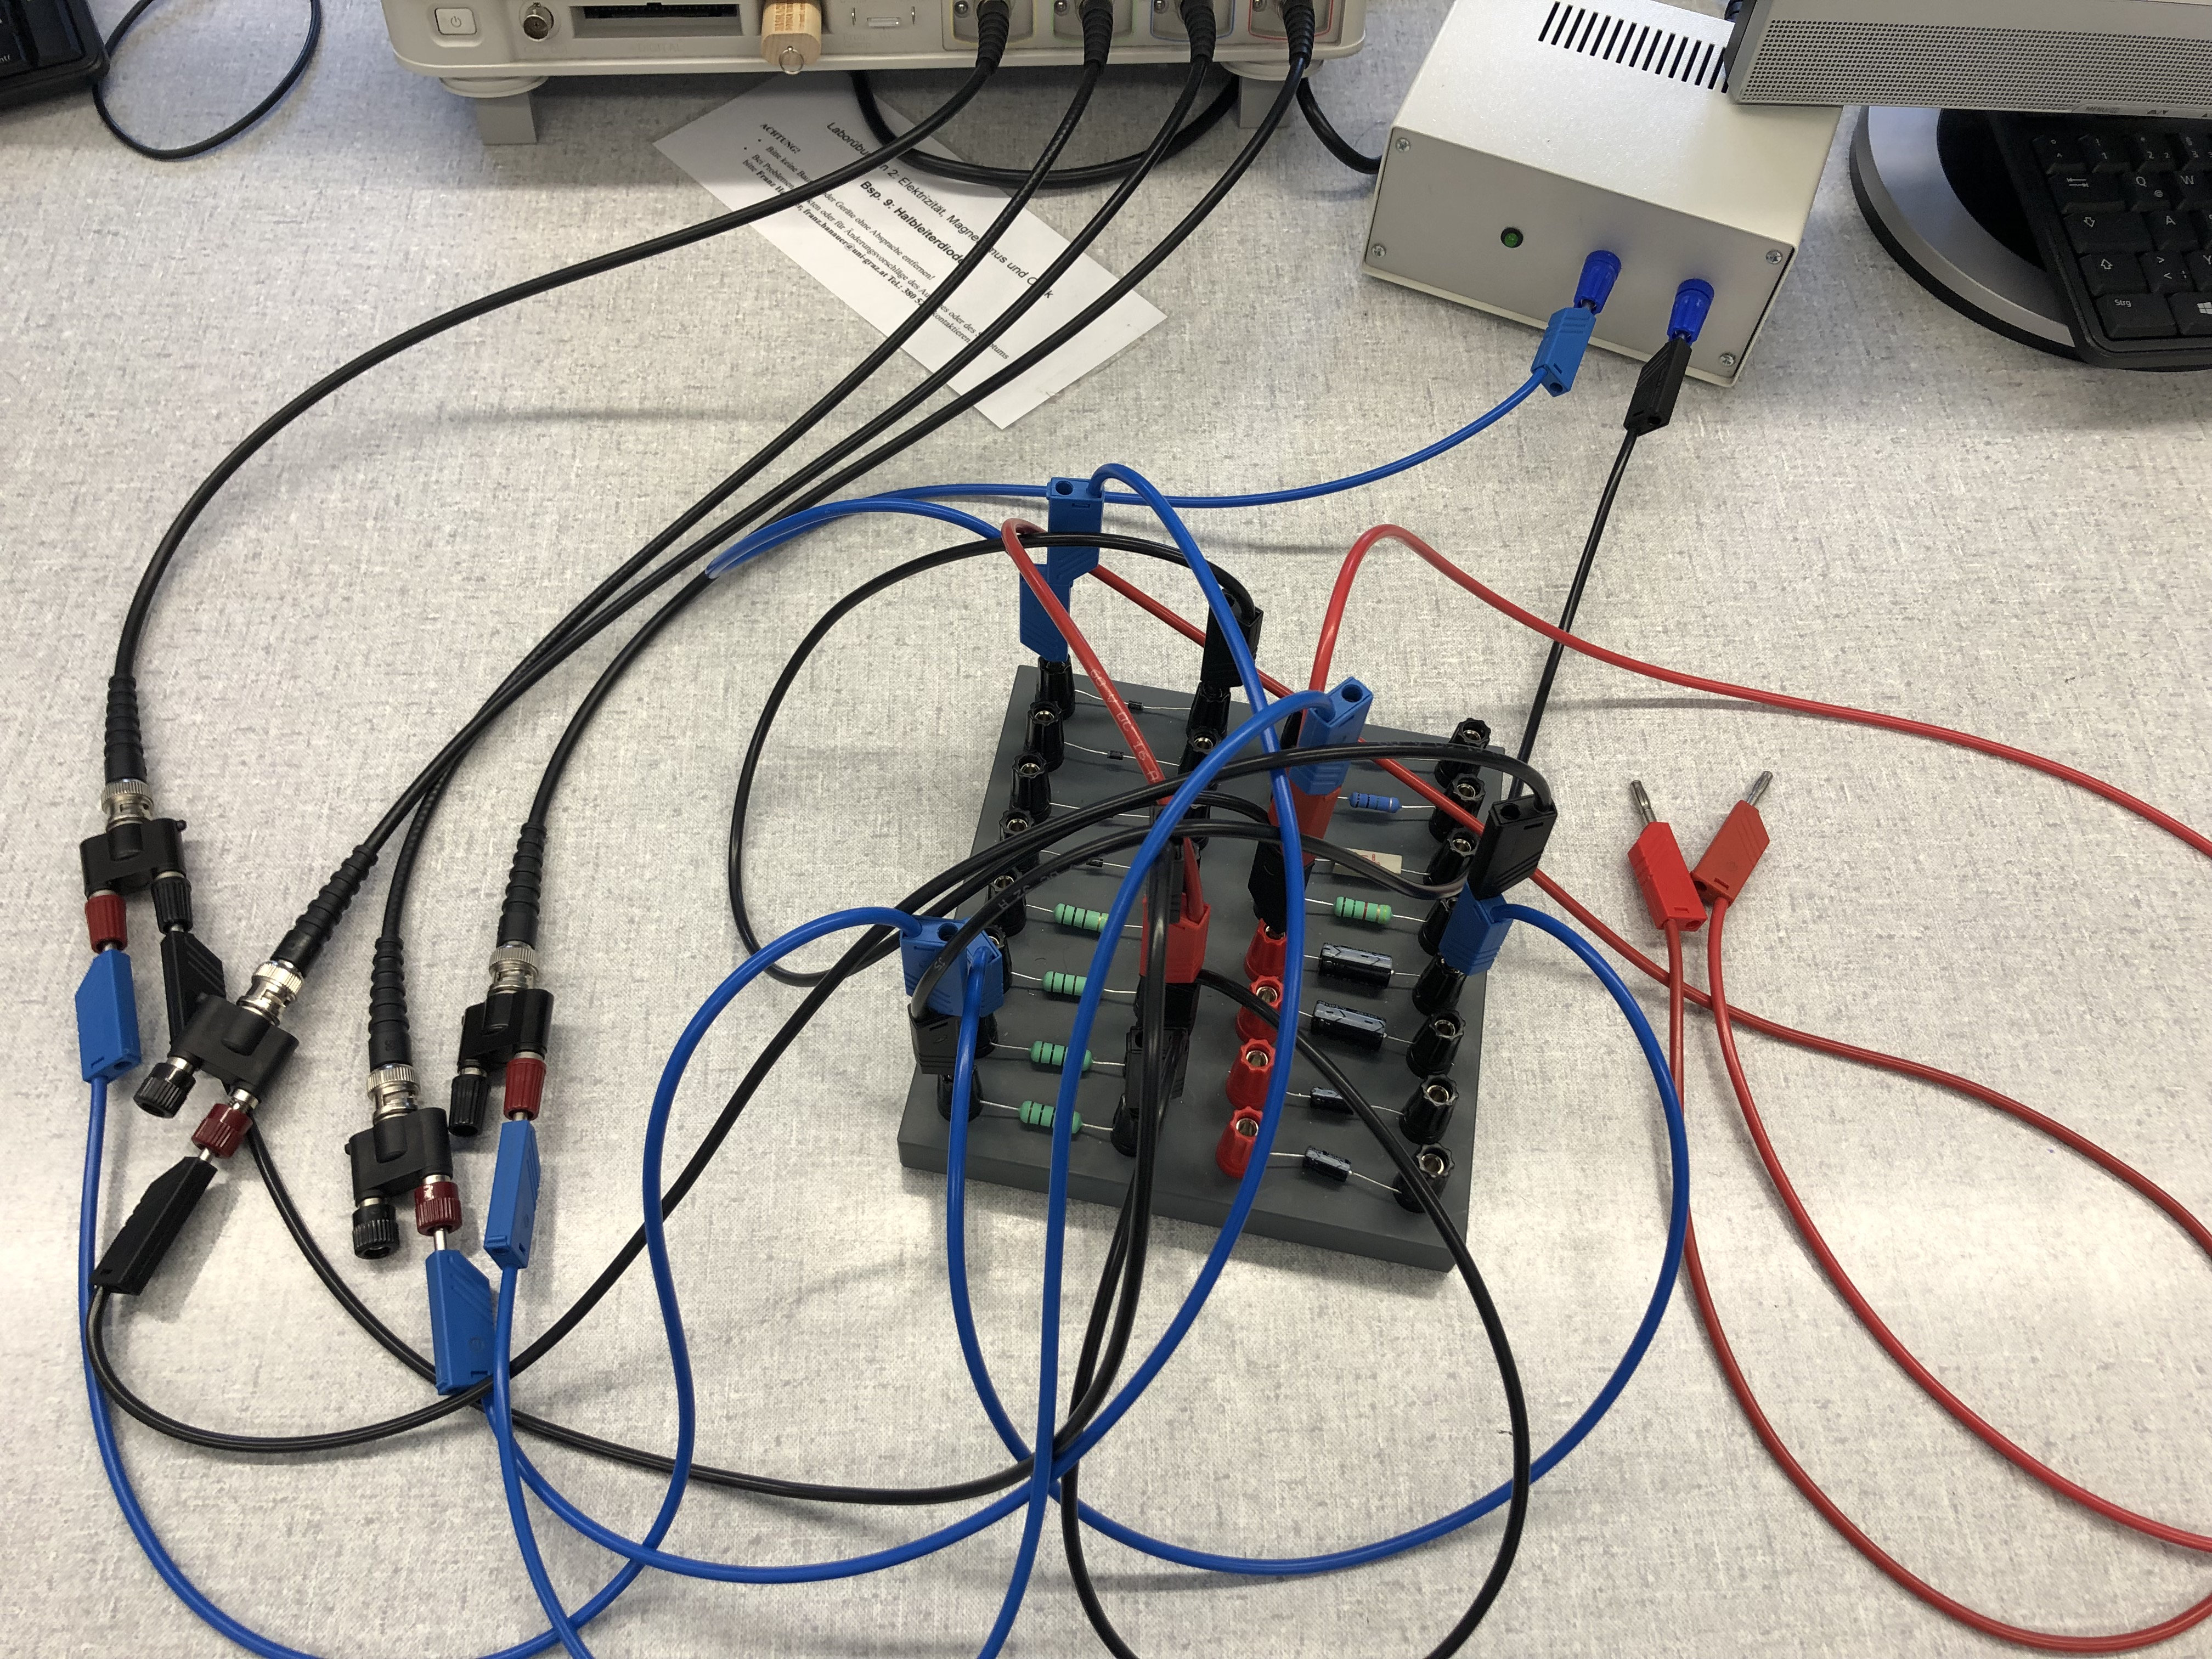
\includegraphics[width=\textwidth]{aufbau3}
		\captionof{figure}{Versuchsaufbau für die Ermittlung der Strom- und Spannungsverläufe mit unterschiedlichen Glättungskondensatoren und Belastungswiderständen}
		\label{fig:aufbau3}
	\end{minipage}
\end{center}

Zunächst wird als Kondensator der Elektrolyt-Kondensator mit 10 $\mu$ Farad benutzt. Der Widerstand R3 wird im Verlauf des Versuchs durch Umstecken der roten Kabel variiert. Zunächst wird dieser als $\infty$ angenommen, was durch Trennen der beiden Kabel erreicht wird. Das dabei vom Oszilloskop erfasste Signal ist in folgender \autoref{fig:oszi_ohne} sichtbar.

\begin{center}
	\begin{minipage}[t]{0.8\textwidth}
		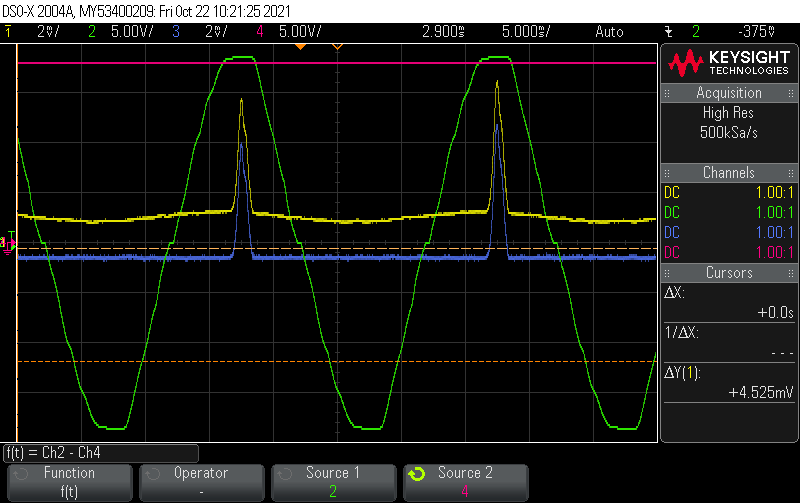
\includegraphics[width=\textwidth]{Halbleiter/scope_2}
		\captionof{figure}{Vom Oszilloskop aufgezeichnete Daten bei einen $\infty$ Widerstand}
		\label{fig:oszi_ohne}
	\end{minipage}
\end{center}

Nun werden der Reihe nach zunächst der Widerstand von \SI{1509(15)}{} $\Omega$,
siehe \autoref{fig:oszi_1500} und schließlich mit einem Widerstand von
\SI{99.2(11)}{\ohm}, siehe \autoref{fig:oszi_100}, mithilfe der roten
Kabel in den Aufbau geschlossen. Die genauen Werte der Widerstände wurden
dabei, wie bereits erwähnt mithilfe des Multimeters zuvor gemessen. Alle vom
Oszilloskop aufgezeichneten Daten wurden auch als CSV-Datei gespeichert, um für
spätere Auswertungen zur Verfügung zu stehen.

\begin{center}
	\begin{minipage}[t]{0.8\textwidth}
		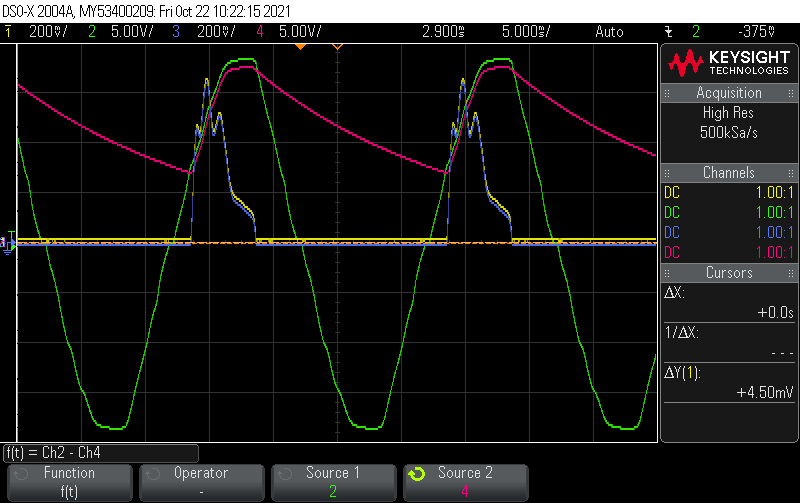
\includegraphics[width=\textwidth]{Halbleiter/scope_3}
		\captionof{figure}{Vom Oszilloskop aufgezeichnete Daten bei einen Widerstand von \SI{1509(15)}{} $\Omega$}
		\label{fig:oszi_1500}
	\end{minipage}
\end{center}

\begin{center}
	\begin{minipage}[t]{0.8\textwidth}
		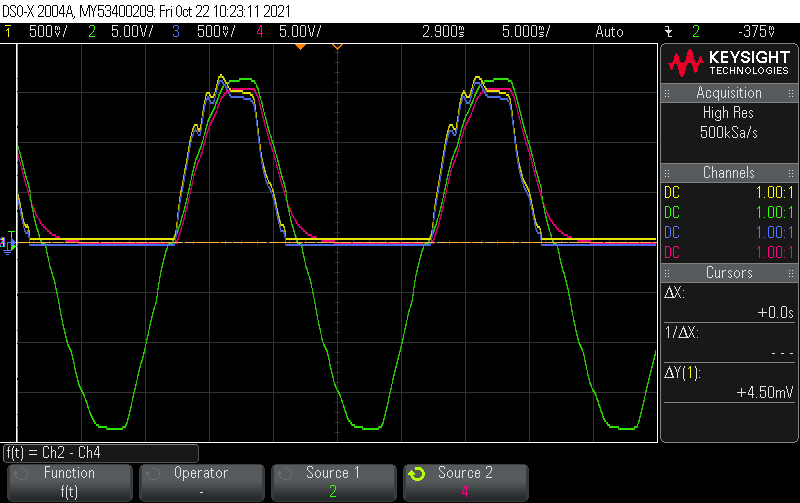
\includegraphics[width=\textwidth]{Halbleiter/scope_6}
		\captionof{figure}{Vom Oszilloskop aufgezeichnete Daten bei einen Widerstand von \num{99.2(11)} $\Omega$}
		\label{fig:oszi_100}
	\end{minipage}
\end{center}

Nun wurde der gesamte Versuch auch mit dem Elektrolyt-Kondensator mit 100 $\mu$ Farad wiederholt, um den Unterschied für die Welligkeit bei einen größeren Kondensator festzustellen.
Um den Rahmen dieses Protokolls nicht zu sprengen werden diese erhaltenen Daten bei der Auswertung unten angeführt und verglichen.


\subsection{Untersuchung der Spannungsverläufe in einer Spannungsverdopplerschaltung}

Zuletzt wird noch der Spannungsverlauf einer Spannungsverdopplerschaltung untersucht. Dazu wird der Stromkreis nach folgenden Schaltplan in \autoref{fig:4} aufgebaut, der der Greinacher-Schaltung entspricht.

\begin{center}
	\begin{minipage}[t]{0.7\textwidth}
		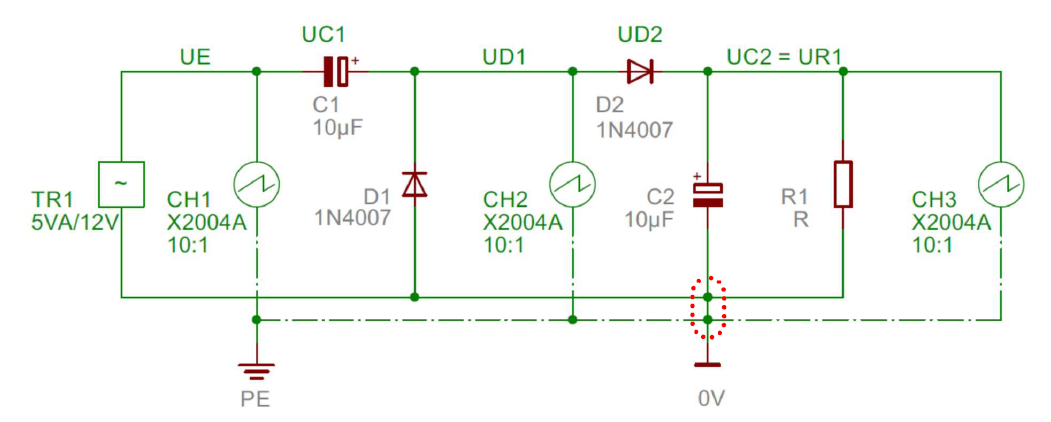
\includegraphics[width=\textwidth]{skizze_4}
		\captionof{figure}{Skizze des Schaltplans für die Greinacher-Schaltung \cite{halbleitervorlage}}
		\label{fig:4}
	\end{minipage}
\end{center}

%Punkte bei 5.4 anschreiben abb 23

\noindent Der tatsächliche Aufbau ist in folgender \autoref{fig:aufbau4} sichtbar. Hier wird auch sichtbar, wie die Tastkabel in die Schaltung integriert werden.

\begin{center}
	\begin{minipage}[t]{0.45\textwidth}
		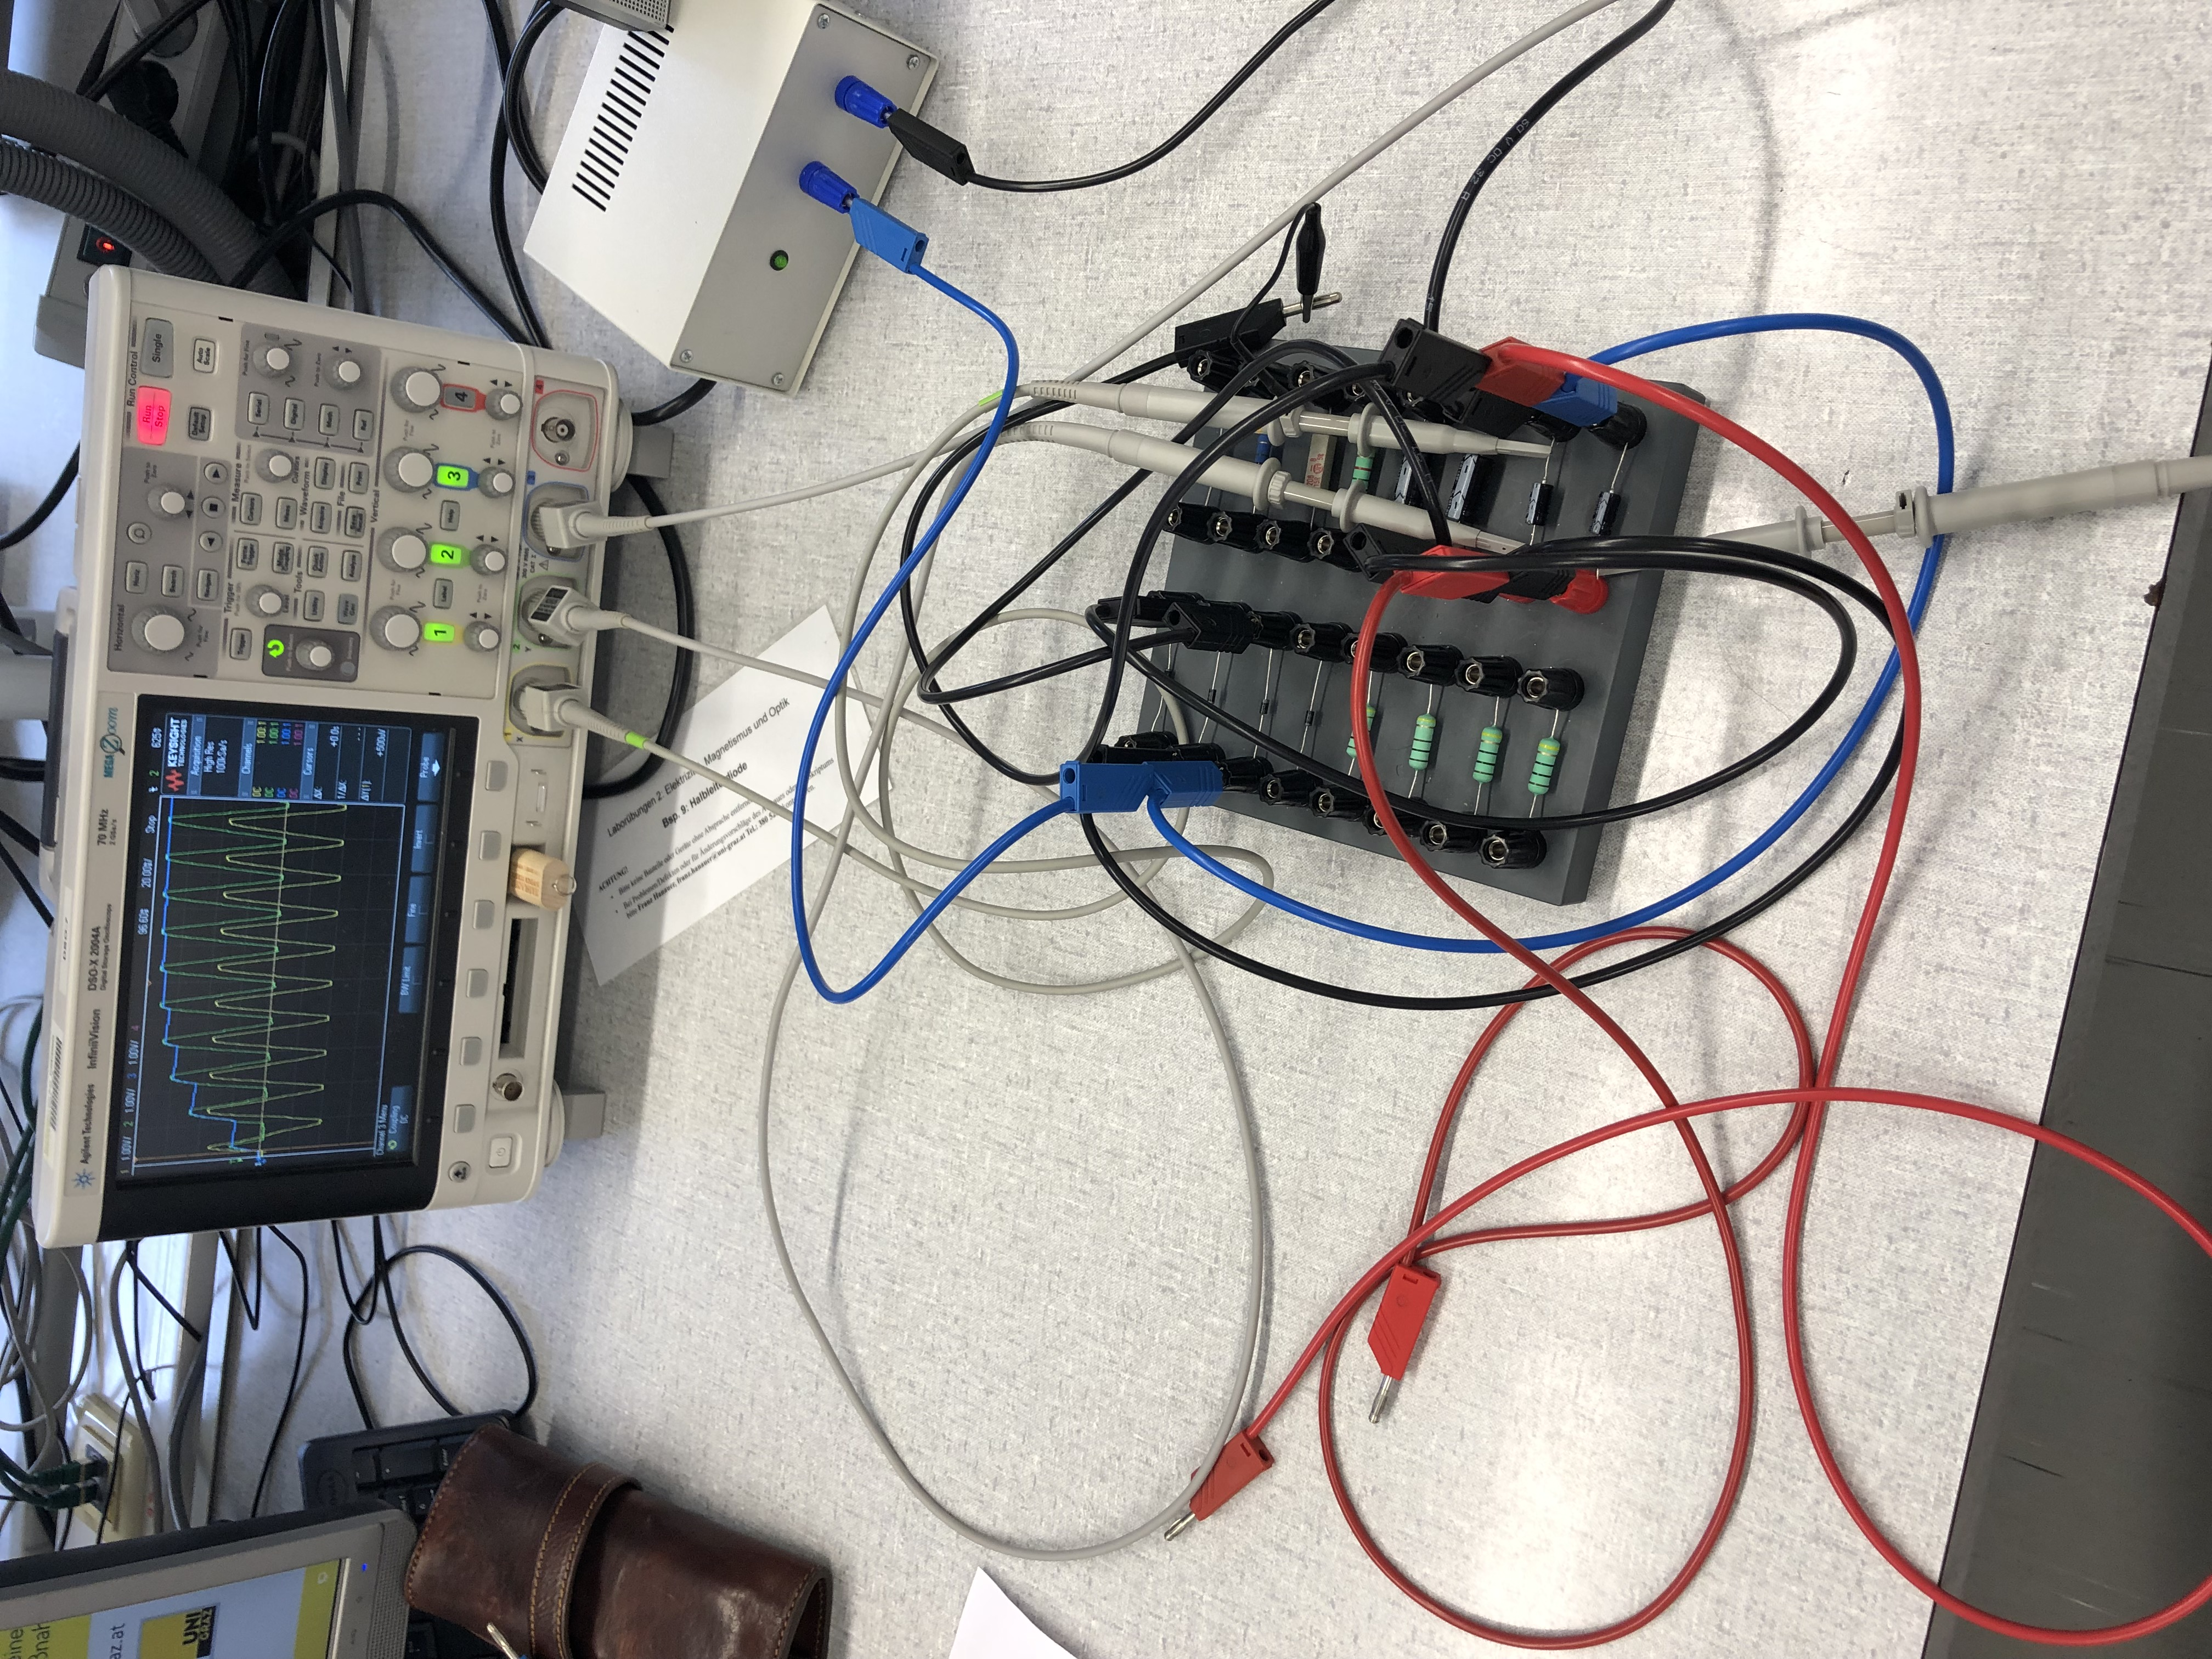
\includegraphics[angle = -90,width=\textwidth]{aufbau4}
		\captionof{figure}{Versuchsaufbau für die Ermittlung des Spannungsverlaufs einer Spannungsverdopplerschaltung}
		\label{fig:aufbau4}
	\end{minipage}
\end{center}

Auch bei der Greinacher-Schaltung werden die roten Kabel wieder verwendet, um den Widerstand R1 zu variieren. Wie bereits zuvor erwähnt, wird auch hier wieder nur ein ``single-shot``, zur Entlastung des Trafos, aufgenommen.

Nun wird der Widerstand R1 zunächst als $\infty$ angenommen, was wie bereits erklärt durch Trennung der roten Kabel erreicht wird, was in \autoref{fig:oszi_4ohne} sichtbar ist.

\begin{center}
	\begin{minipage}[t]{0.8\textwidth}
		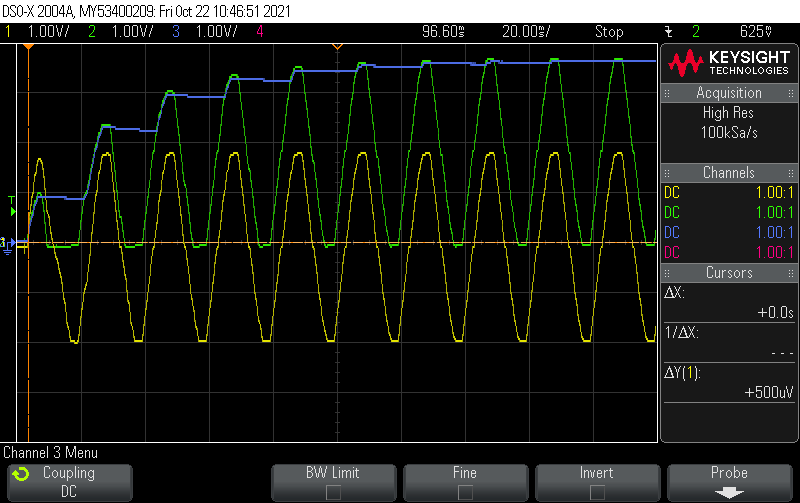
\includegraphics[width=\textwidth]{Halbleiter/scope_15}
		\captionof{figure}{Vom Oszilloskop aufgezeichnete Daten bei Greinacher-Schaltung und einem $\infty$ Widerstand}
		\label{fig:oszi_4ohne}
	\end{minipage}
\end{center}

Nun wird mithilfe der roten Kabel ein Widerstand von \SI{1509(15)}{} $\Omega$, siehe \autoref{fig:oszi_41500}, in die Schaltung geschlossen.

\begin{center}
	\begin{minipage}[t]{0.8\textwidth}
		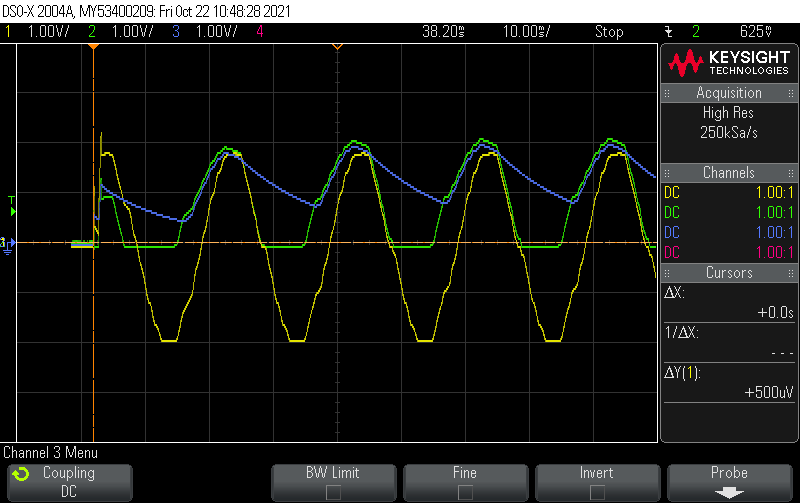
\includegraphics[width=\textwidth]{Halbleiter/scope_16}
		\captionof{figure}{Vom Oszilloskop aufgezeichnete Daten bei Greinacher-Schaltung und einem Widerstand von \SI{1509(15)}{} $\Omega$}
		\label{fig:oszi_41500}
	\end{minipage}
\end{center}




\section{Auswertung}

\noindent Um zu sehen wie sich die Unsicherheit der Messungen bis in die Ergebnisse
fortplanzt, ist \autoref{eq:Unsicherheitsfortpflanzung} verwendet worden.
Die Grundlagen dieser Gleichung stammen von den Powerpointfolien von
GUM.\cite{WolfgangKessel2004} Die Verallgemeinerung ist von Wikipedia entnommen
worden \cite{2020Fehler}.
Für die Auswertung ist die Progammiersprache Python im speziellen das
Packet \verb#scipy#, zur Hilfe genommen worden.

\begin{equation}
	\label{eq:Unsicherheitsfortpflanzung}
	V_y = J(x) \cdot V_x \cdot J^{T}(x)
\end{equation}

\noindent Wobei $V_y$ und $V_x$ die Kovarianzmatrizen von den Vektoren $\bm{y}$ und $\bm{x}$ sind.
$\bm{x}$ ist der Vektor der Eingangsvariablen und $\bm{y}$ ist der Vektor der Ausgangsvariablen.
$J$ ist die Jakobimatrix der vektorwertigen Funktion $\bm{y} = \vec{F}(\bm{x})$.
So lassen sich die Komponenten der Matrix relativ einfach anschreiben $J_{ij}(x) = \frac{\partial{y_i}}{\partial{x_j}}(x)$.
Damit man die Unsicherheit der einzelnen Variablen $y_i$ bekommt, muss nur die Quadratwurzel des i-ten Diagonalelementes der
$\bm{y}$-Kovarianzmatrix genommen werden $u_i= \sqrt{\mathrm{diag}(V_y)_i}$.
Da in diesem Experiment meistens nur skalare Funktionen untersucht werden, vereinfacht
sich die \autoref{eq:Unsicherheitsfortpflanzung} dramatisch und die Unsicherheit
der Variable $y$ lässt sich einfach so berechnen:

\begin{equation}
	\label{eq:graduncentainty}
	u_y = \sqrt{\mathrm{grad} y^T \cdot V_x \cdot \mathrm{grad} y}
\end{equation}

\newpage

\subsection{Ermittlung der Strom-Spannungscharakteriskik einer Gleichrichterdiode}

\subsubsection{in Durchlassrichtung}

Um die Strom-Spannungskennlinie der Si-Gleichrichterdiode D1 in
Durchlassrichtung zu ermitteln, wurden die aufgenommenen Daten aufgetragen, was
in folgender \autoref{fig:durchlass} sichtbar ist. Die ebenfalls ersichtlichen
Unsicherheiten wurden dabei anhand des Gerätedatenblatt errechnet. \cite{1n4007}


\begin{center}
	\begin{minipage}[t]{0.8\textwidth}
		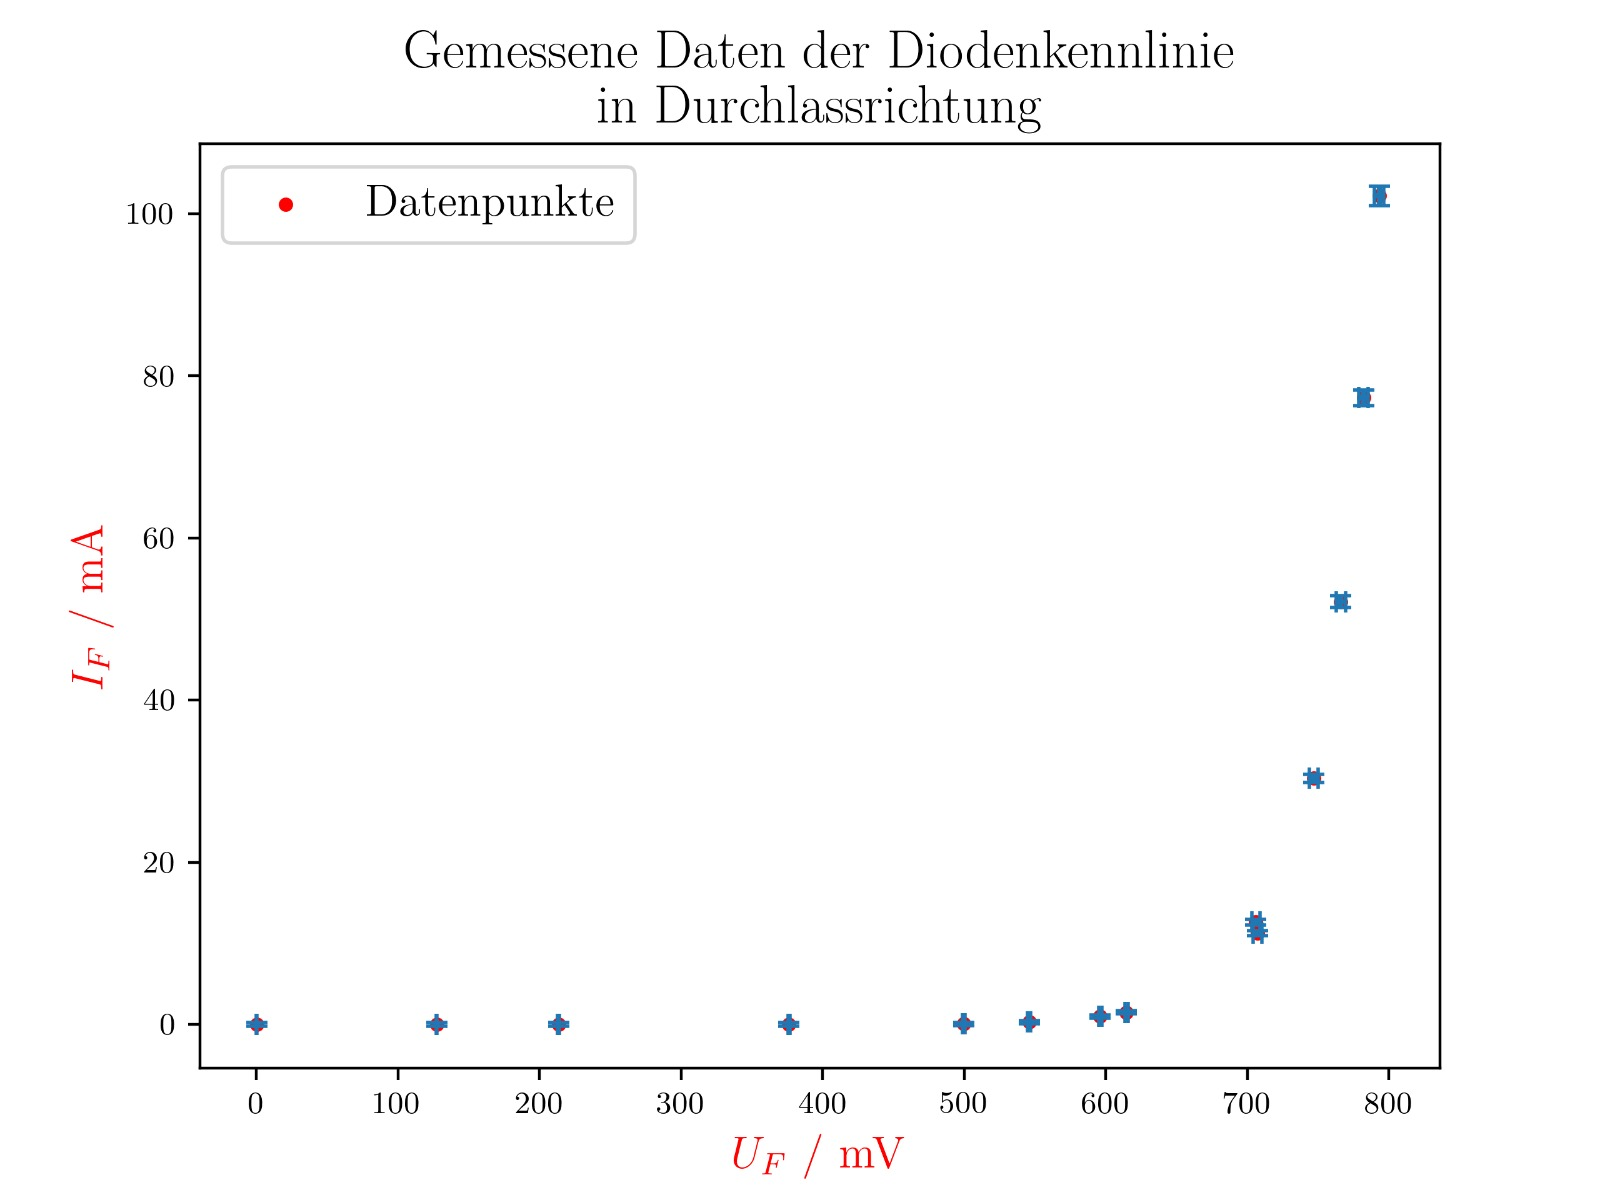
\includegraphics[width=\textwidth]{./figures/halbleiter/Versuch1/durchlass_error}
		\captionof{figure}{Gemessene Daten zur Ermittlung der Diodenkennlinie in Durchlassrichtung}
		\label{fig:durchlass}
	\end{minipage}
\end{center}

\newpage

\subsubsection{in Sperrrichtung}
Um die Strom-Spannungskennlinie der Si-Gleichrichterdiode D1 in Sperrrichtung zu erhalten, werden, wie bereits zuvor, die gemessenen Daten inklusive der Unsicherheiten aus dem Datenblatt geplottet, was in folgender \autoref{fig:sperrrichtung} ersichtlich ist.

\begin{center}
	\begin{minipage}[t]{0.8\textwidth}
		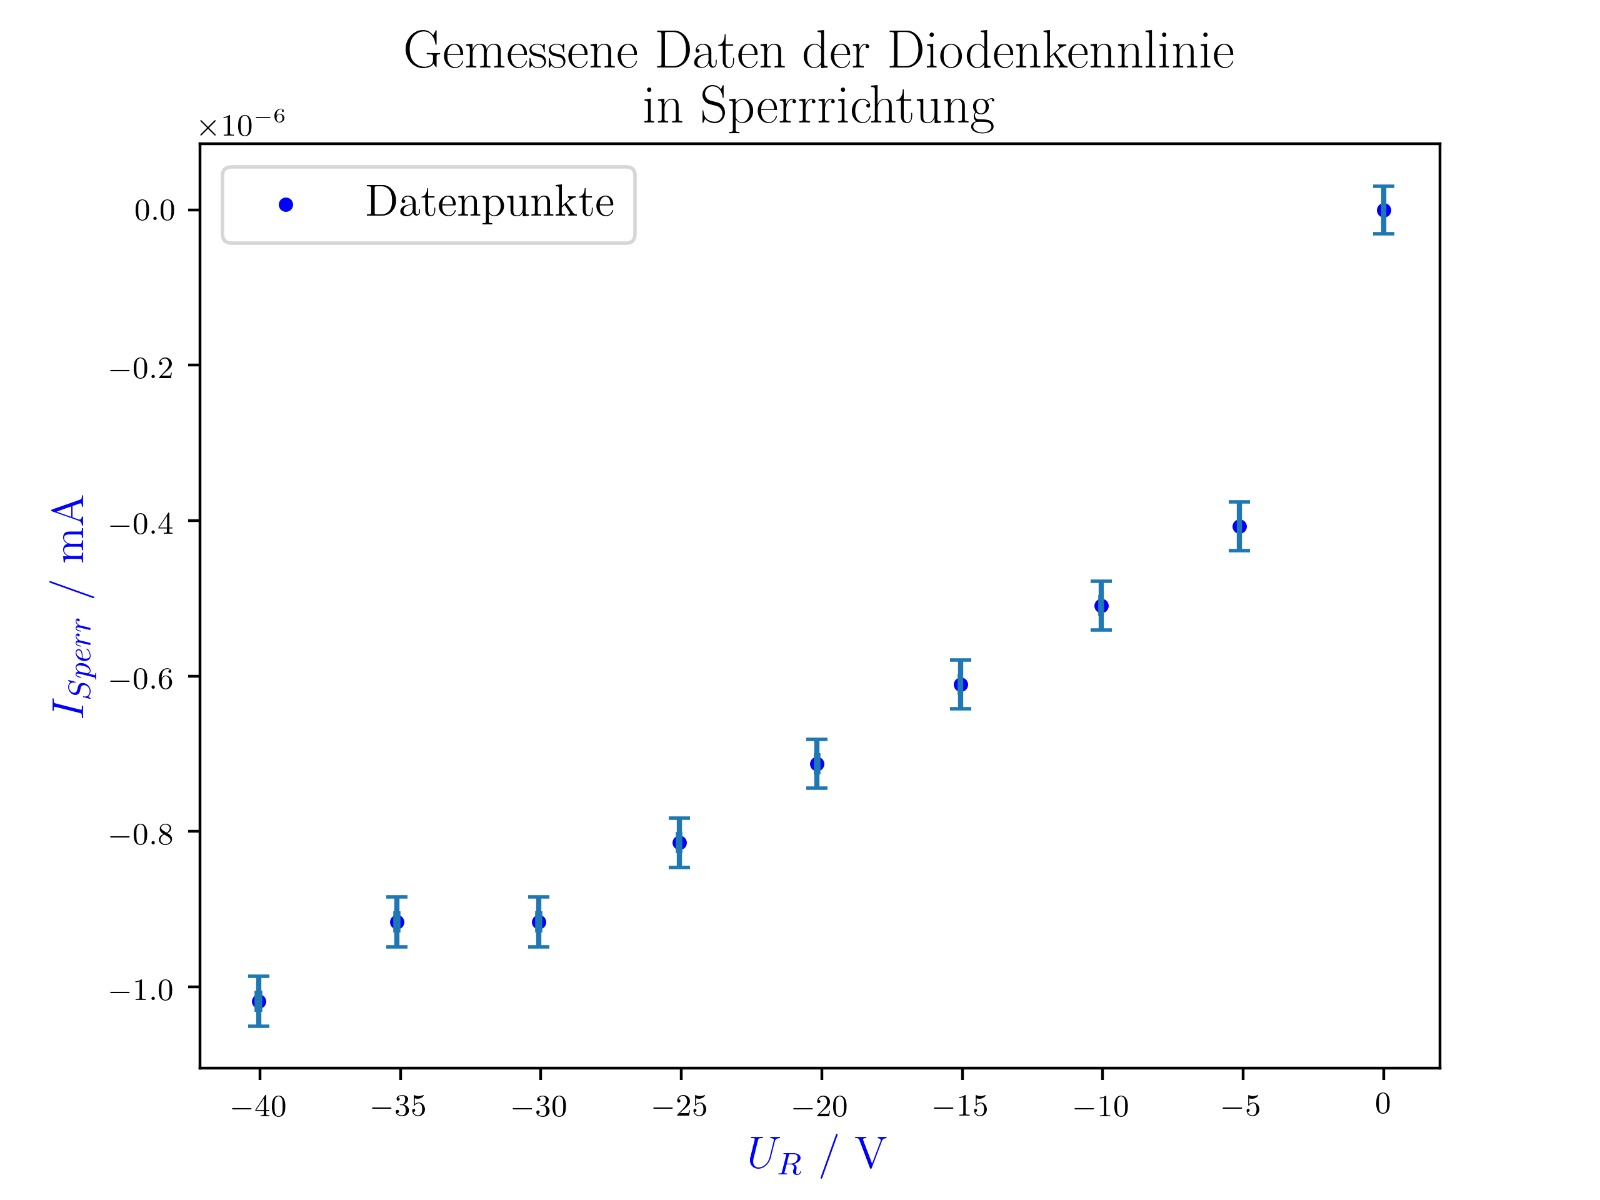
\includegraphics[width=\textwidth]{./figures/halbleiter/Versuch1/sperr_error}
		\captionof{figure}{Gemessene Daten zur Ermittlung der Diodenkennlinie in Sperrrichtung}
		\label{fig:sperrrichtung}
	\end{minipage}
\end{center}

\newpage

\subsection{Ermittlung der Strom-Spannungscharakteriskik einer Zenerdiode}


Um die Strom-Spannungskennlinie der Zenerdiode D1 in Durchlass- und Sperrrichtung zu bestimmen, wurden die gemessenen Daten, die auch in \autoref{fig:oszi2} sichtbar sind und als CSV Datei gespeichert wurden, verwendet. Der Strom der Diode $I_D$ wurde dabei nach folgender Formel bestimmt.

\begin{equation}
	I_D= \frac{U_E-U_{D1}}{R_1}
\end{equation}

Die so erhaltenen Werte wurden, der besseren Übersicht halber, nun interpoliert und so die Diodenkennlinie als I / U aufgetragen, was in  \autoref{fig:diodenkennlinie} ersichtlich ist.

\begin{center}
	\begin{minipage}[t]{0.8\textwidth}
		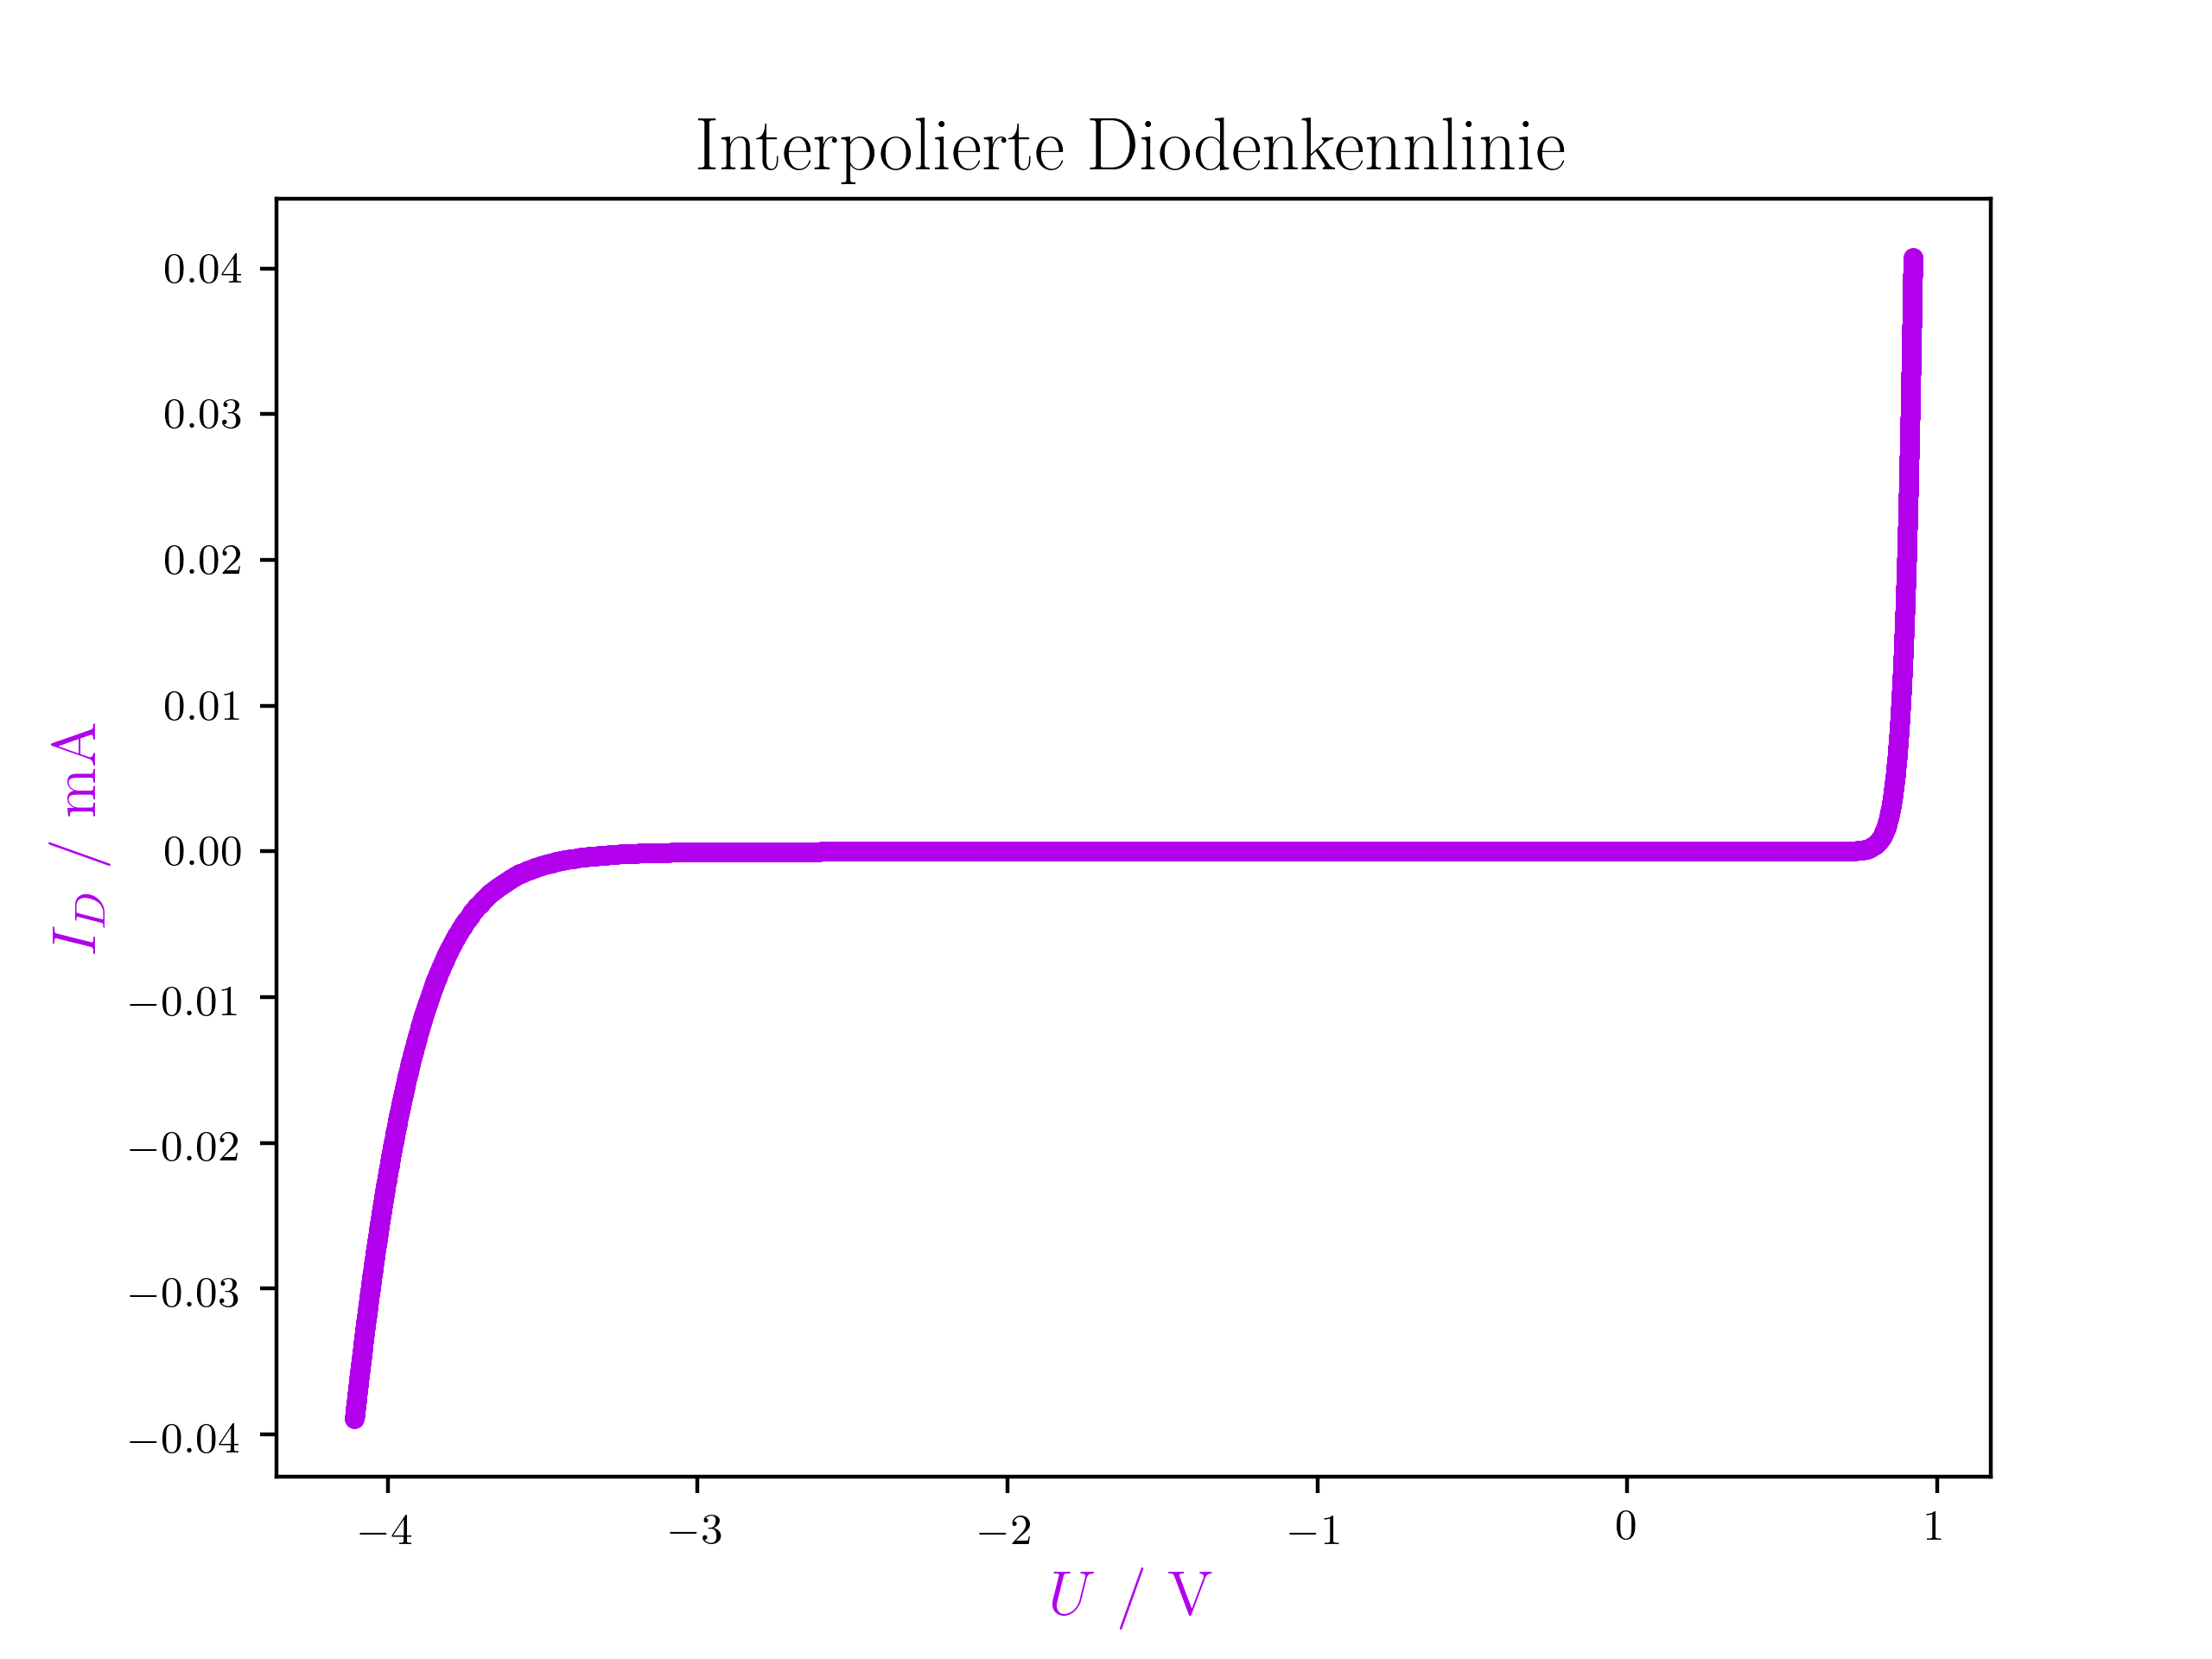
\includegraphics[width=\textwidth]{./figures/halbleiter/Versuch2/diodenkennlinie.png}
		\captionof{figure}{Interpolierte Diodenkennlinie als I / U}
		\label{fig:diodenkennlinie}
	\end{minipage}
\end{center}

\newpage

\subsection{Untersuchung der Strom- und Spannungsverläufe mit unterschiedlichen Glättungskondensatoren und Belastungswiderständen}

Nun wurden die Spannungs- und Stromverläufe grafisch als Funktion der Zeit
über mehrere Perioden dargestellt.

Um die Glättungsfunktion mit Hilfe der Welligkeit zu bewerten, wurde diese zunächst mit \autoref{eq:welligkeit} numerisch bestimmt und
den Grafiken beigefügt.

\begin{equation}
	w = \frac{U_{\sim}}{|U_{-}|} =\frac{\sqrt{\frac{1}{T_2-T_1}\int_{T_1}^{T_2}(u(t)-|U_{-}|)^2 \mathrm{d}t}}{\frac{1}{T_2-T_1}\int_{T_1}^{T_2}|u(t)|\mathrm{d}t}
	\label{eq:welligkeit}
\end{equation}

Die entsprechenden vom Oszilloskop aufgezeichneten Daten der beiden Spannungen $U_{CH2}$ $U_{CH4}$, sichtbar in \autoref{fig:oszi_ohne}, wurden in folgenden Graphen aufgetragen. Zusätzlich wurde $U_{D1}=U_{CH2}-U_{CH4}$ berechnet und auch in den selben Graphen gezeichnet, wodurch folgende \autoref{fig:spannunginf} entsteht.

\begin{center}
	\begin{minipage}[t]{0.8\textwidth}
		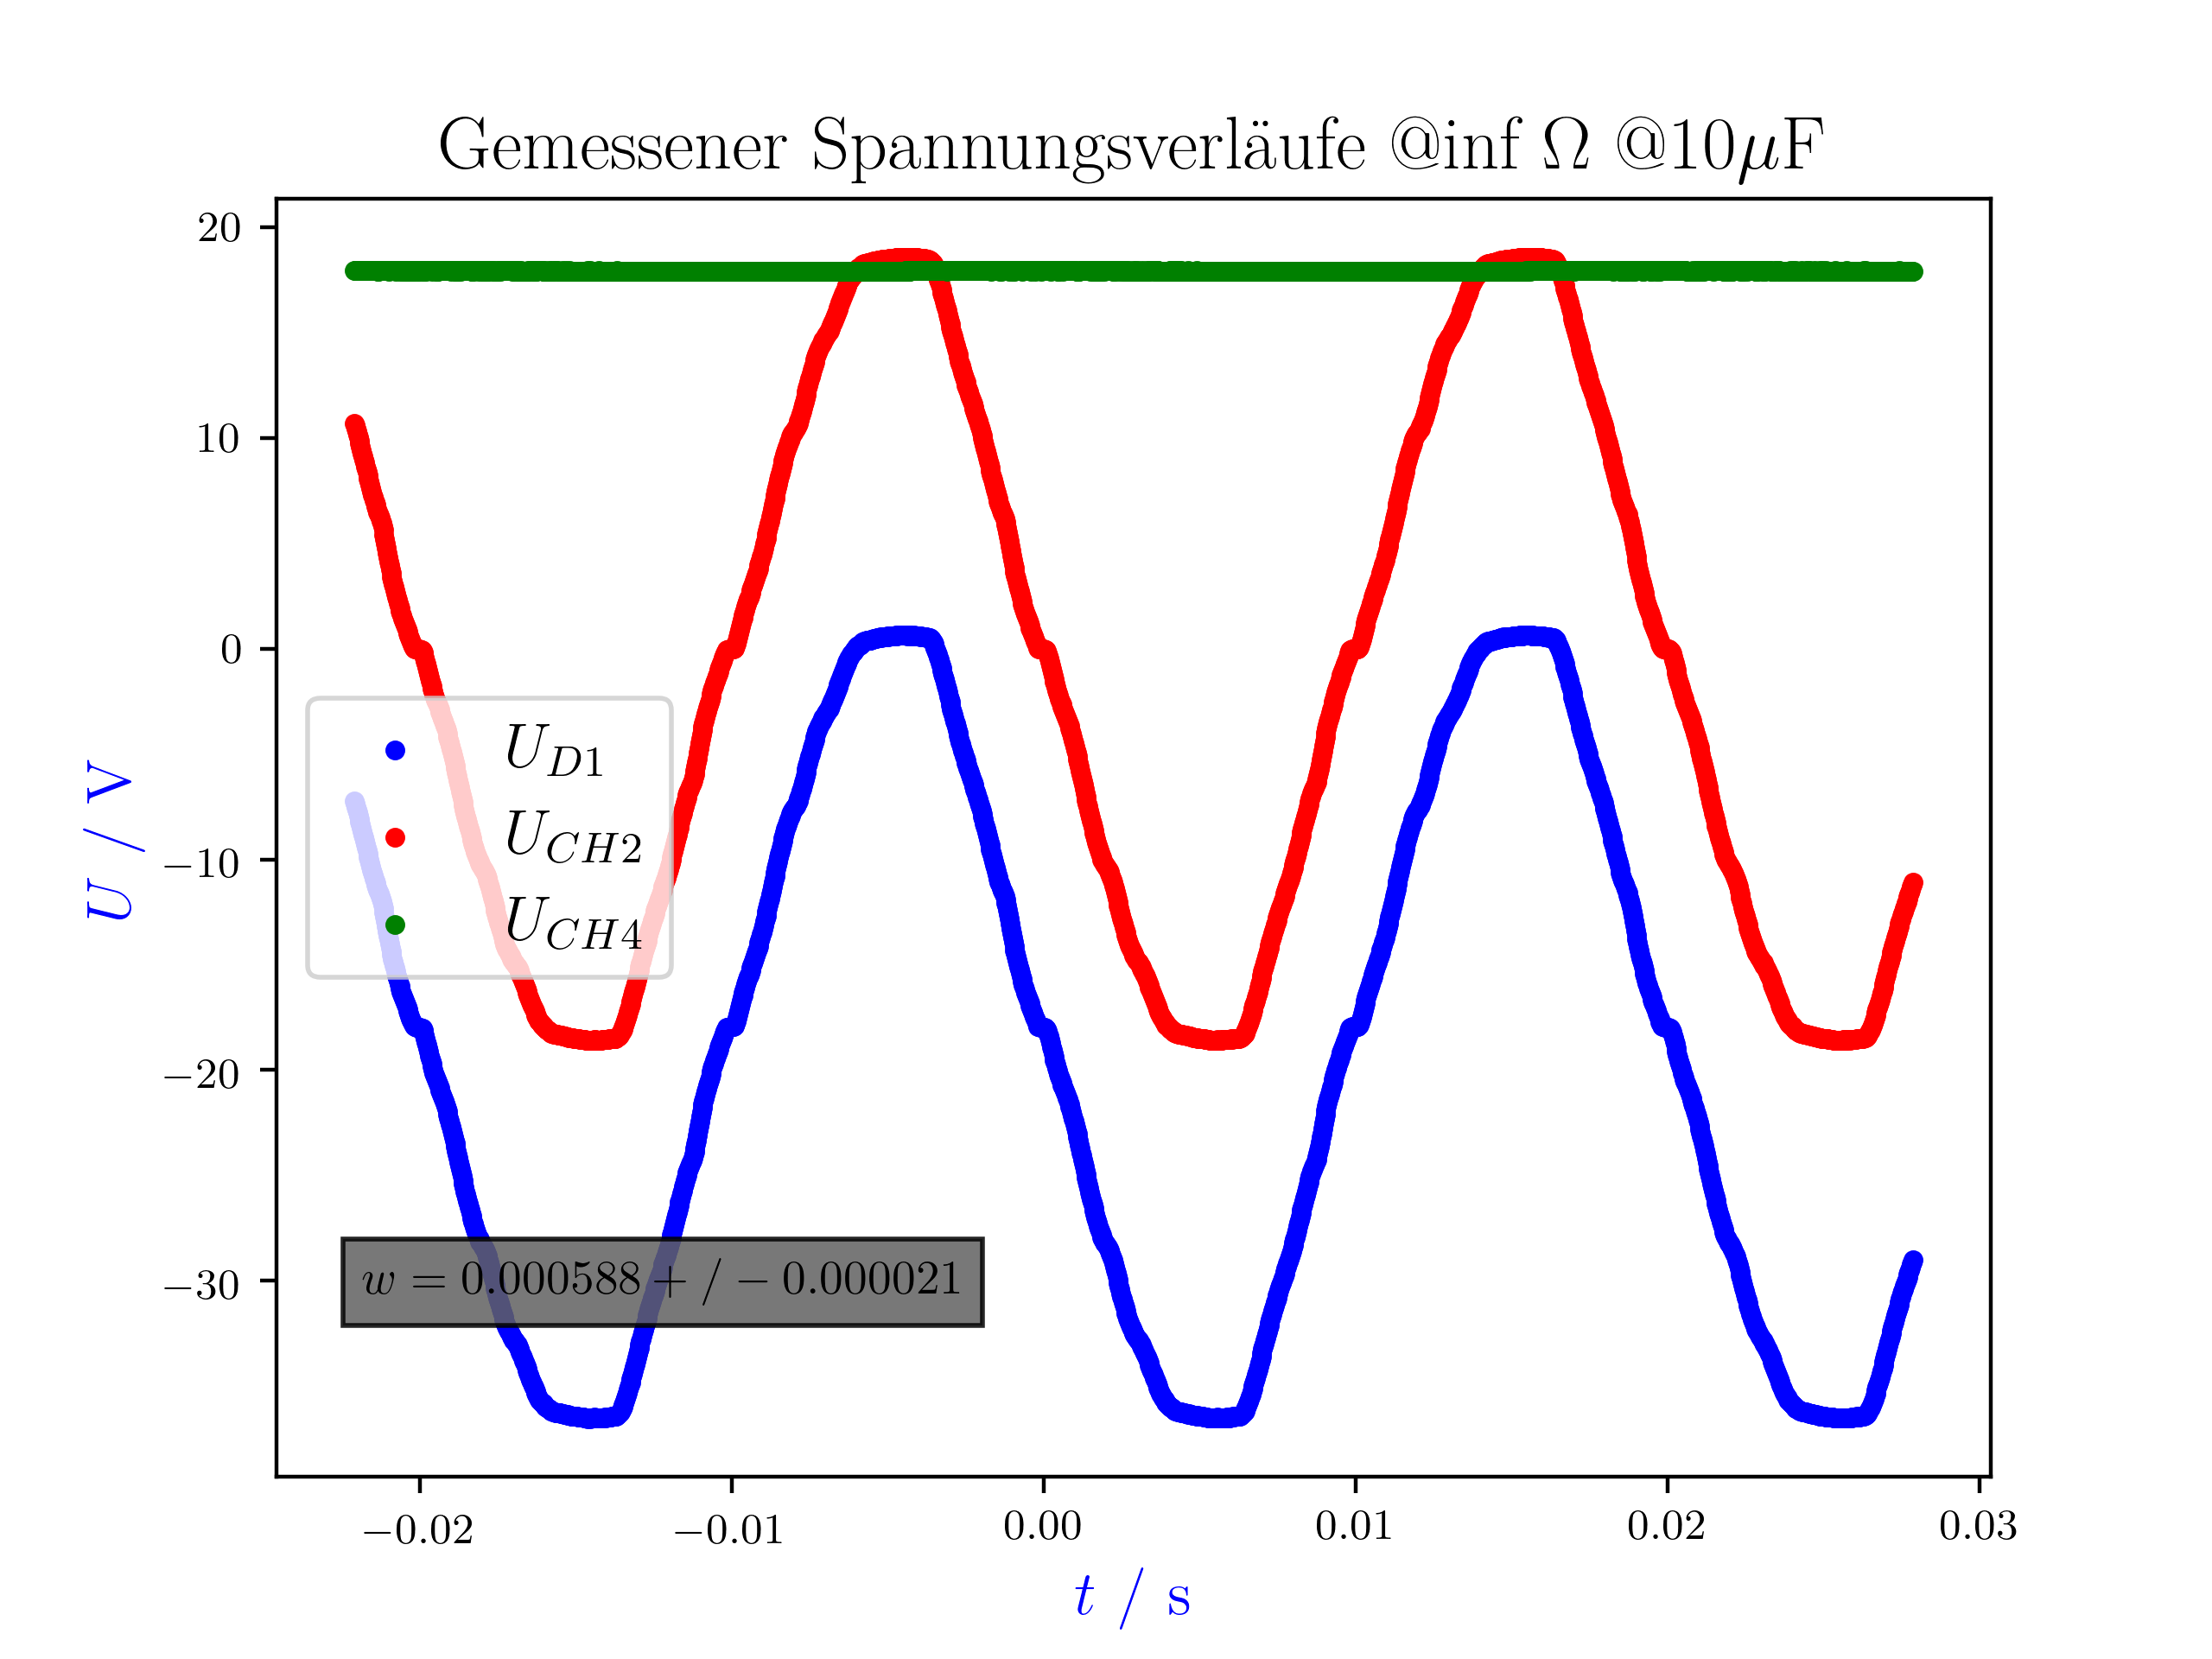
\includegraphics[width=\textwidth]{./figures/halbleiter/Versuch3/spannunginf.png}
		\captionof{figure}{Erhaltene Spannungsverläufe bei einem Kondensator mit einer Kapazität von 10 $\mu$ Farad und einem $\infty$ großen Widerstand}
		\label{fig:spannunginf}
	\end{minipage}
\end{center}

Dieser Vorgang wird nun für die anderen beiden Widerstände wiederholt.

\begin{center}
	\begin{minipage}[t]{0.8\textwidth}
		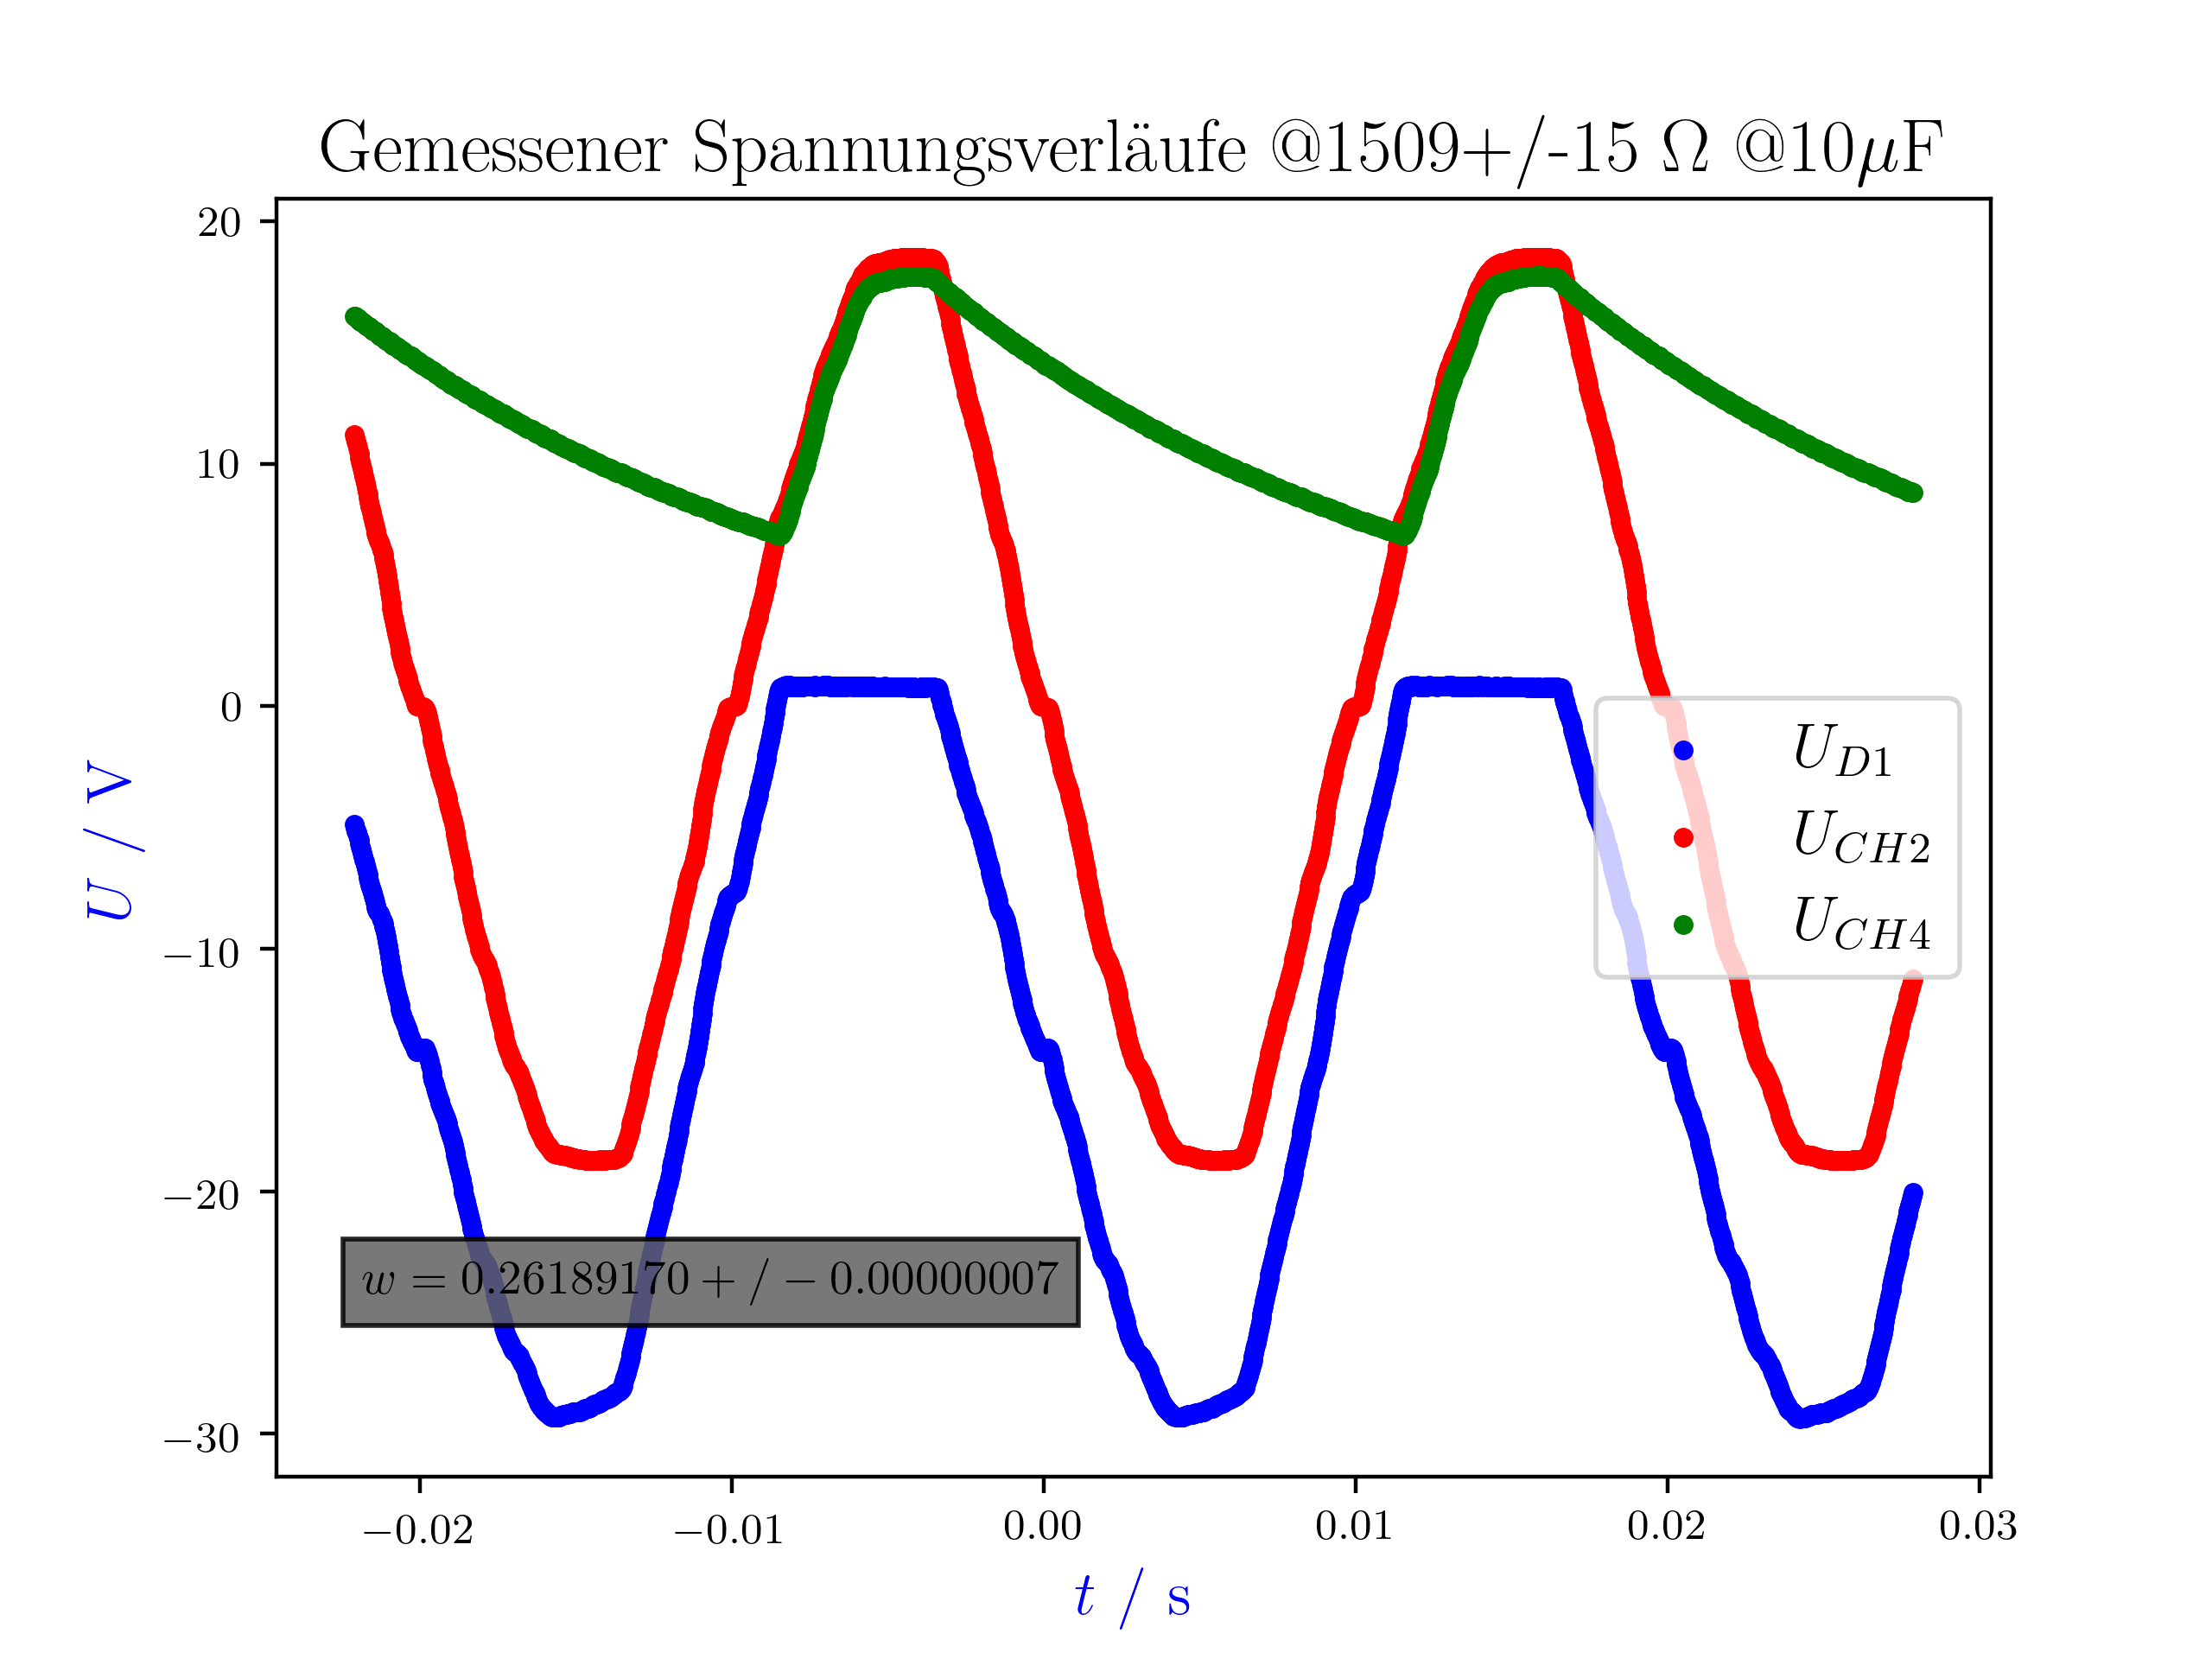
\includegraphics[width=\textwidth]{./figures/halbleiter/Versuch3/spannung1509.0.png}
		\captionof{figure}{Erhaltene Spannungsverläufe bei einem Kondensator mit einer Kapazität von 10 $\mu$ Farad und einem Widerstand von \SI{1509(15)}{}$\Omega$}
		\label{fig:spannung1509}
	\end{minipage}
\end{center}

\begin{center}
	\begin{minipage}[t]{0.8\textwidth}
		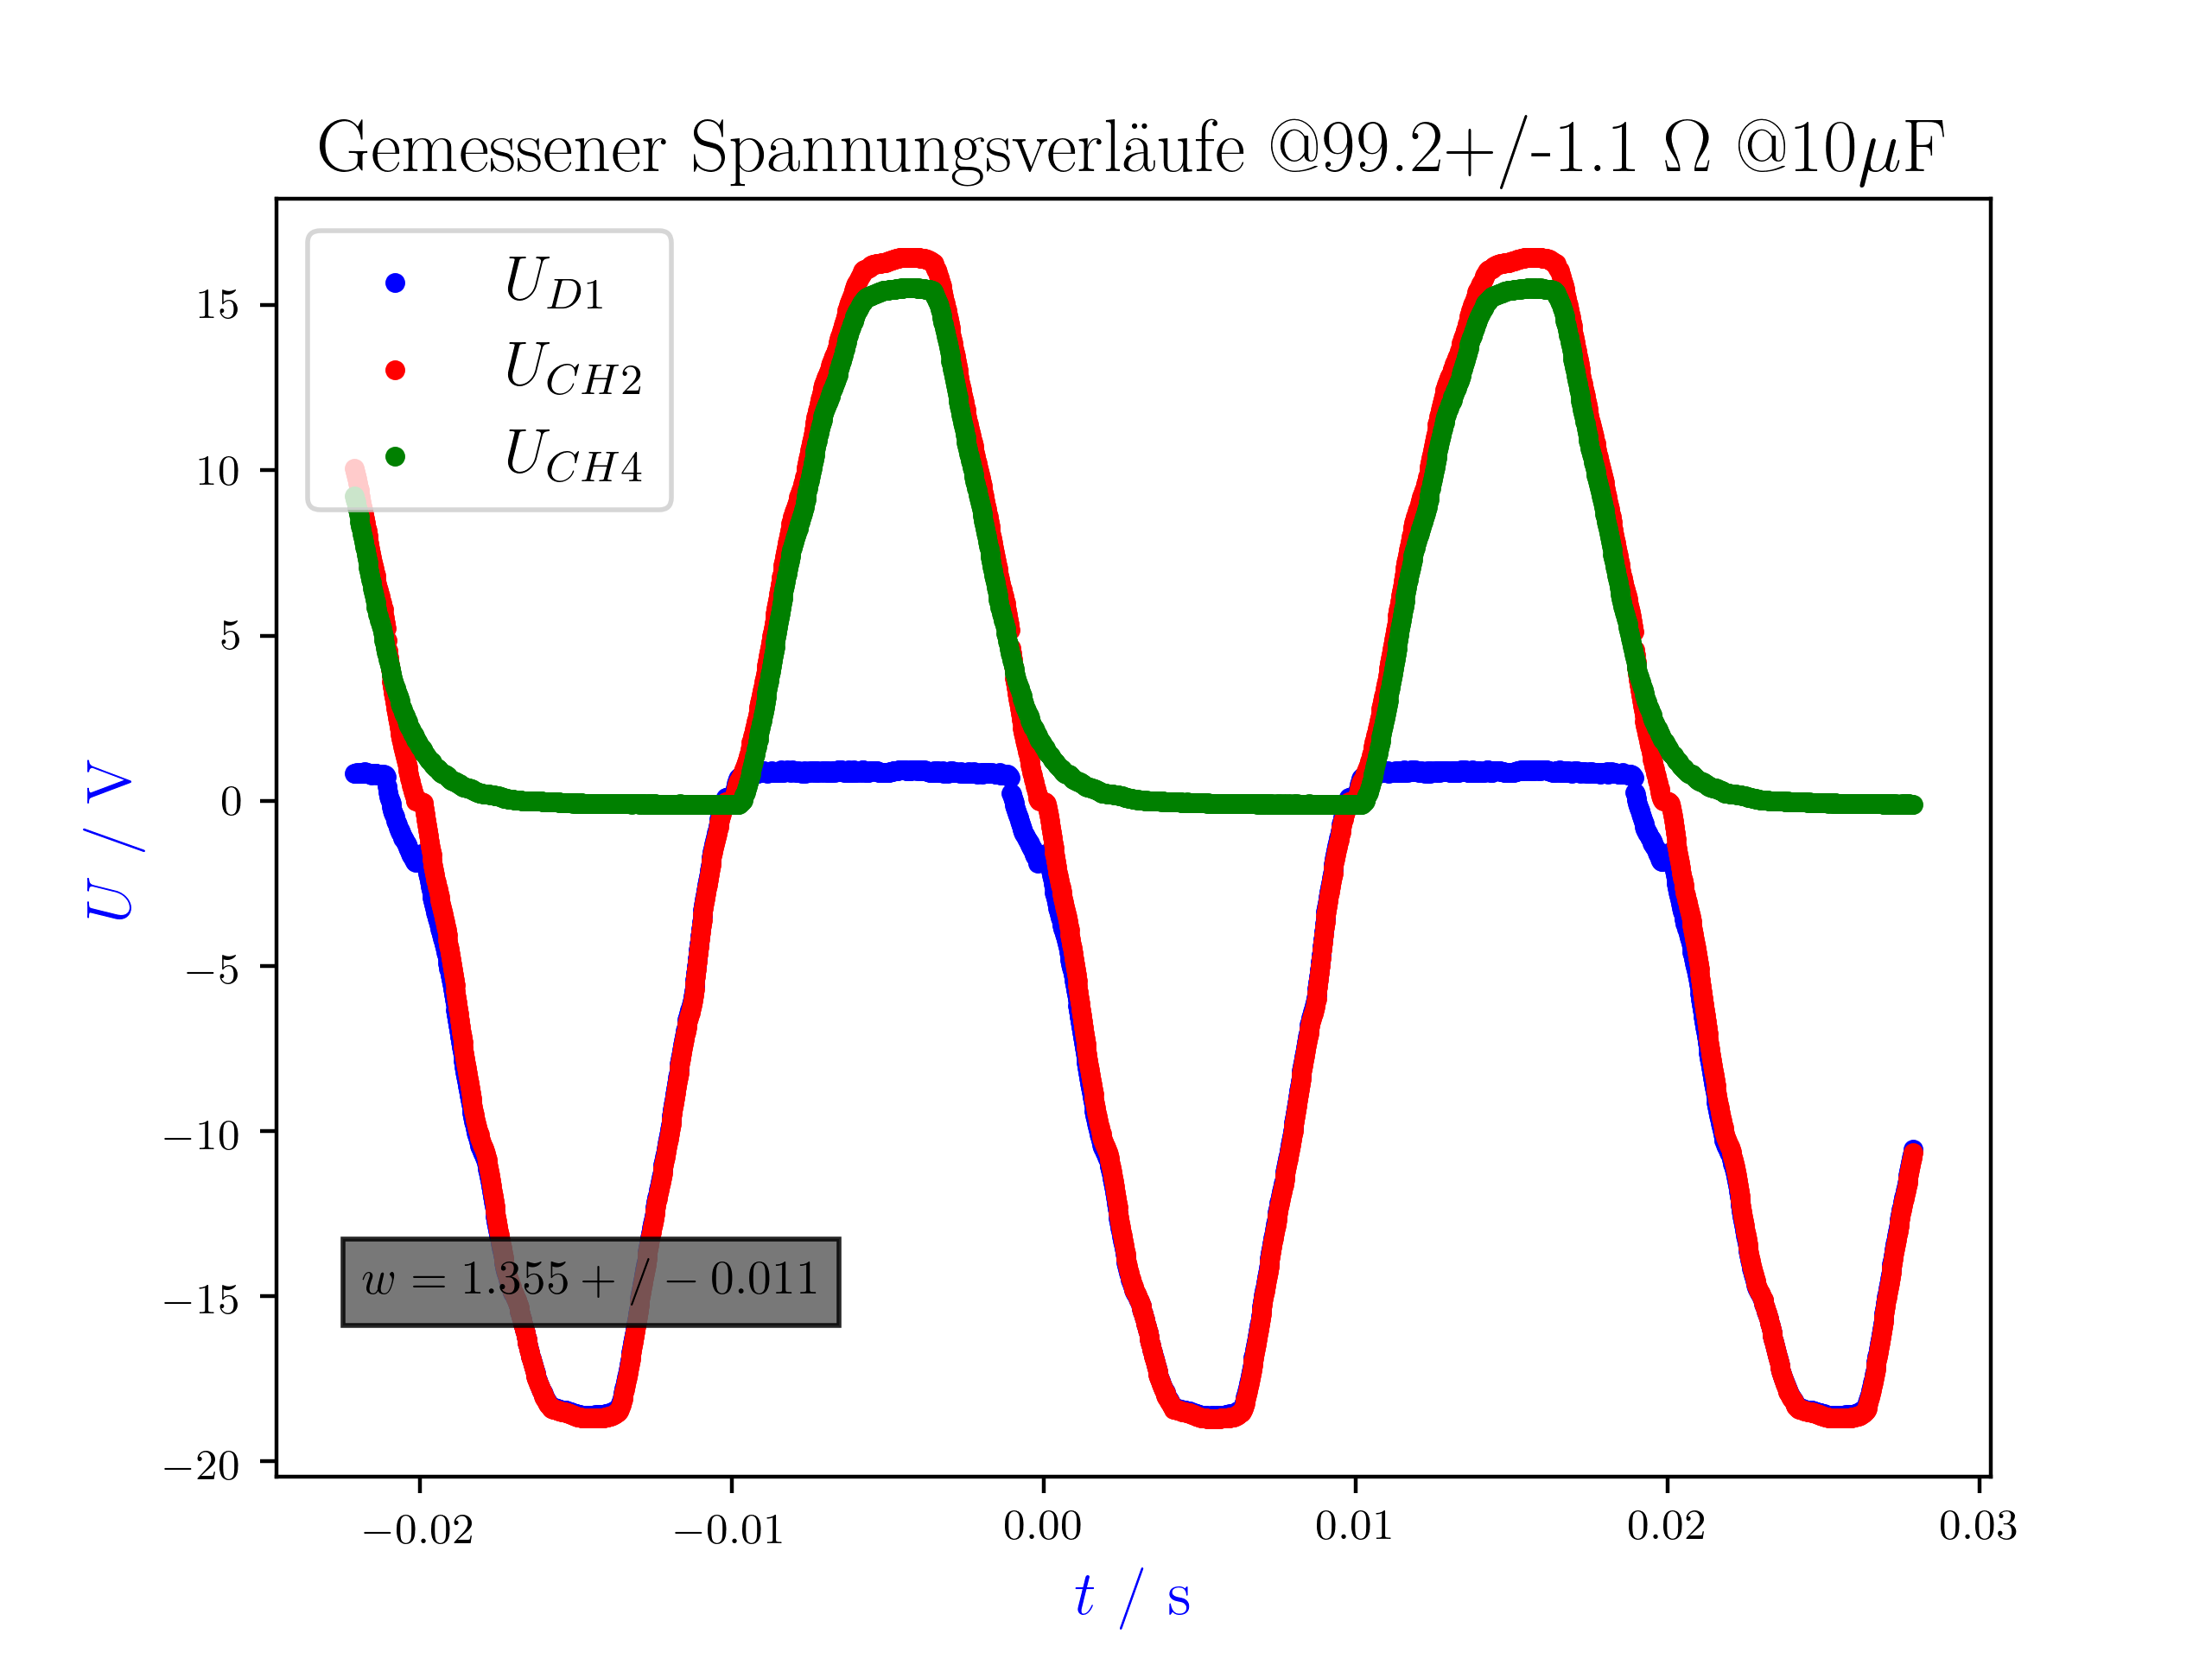
\includegraphics[width=\textwidth]{./figures/halbleiter/Versuch3/spannung99.2.png}
		\captionof{figure}{Erhaltene Spannungsverläufe bei einem Kondensator mit einer Kapazität von 10 $\mu$ Farad und einem Widerstand von \num{99.2(11)} $\Omega$}
		\label{fig:spannung100}
	\end{minipage}
\end{center}

\newpage

Die Ströme $I$ wurden nach folgenden Formeln berechnet.

\begin{equation}
	I_{R1}=I_{D1}=\frac{U_{CH1}}{R_1} \quad \quad I_{R3}=\frac{U_{CH4}}{R_3} \quad \quad I_{C1}=\frac{U_{CH3}}{R_2}
\end{equation}

Die so erhaltenen Werte der Ströme wurden in Graphen veranschaulicht und sind im Folgenden ersichtlich.

\vspace{2mm}

Dies wurde wieder für alle drei Widerstände wiederholt.

\begin{center}
	\begin{minipage}[t]{0.8\textwidth}
		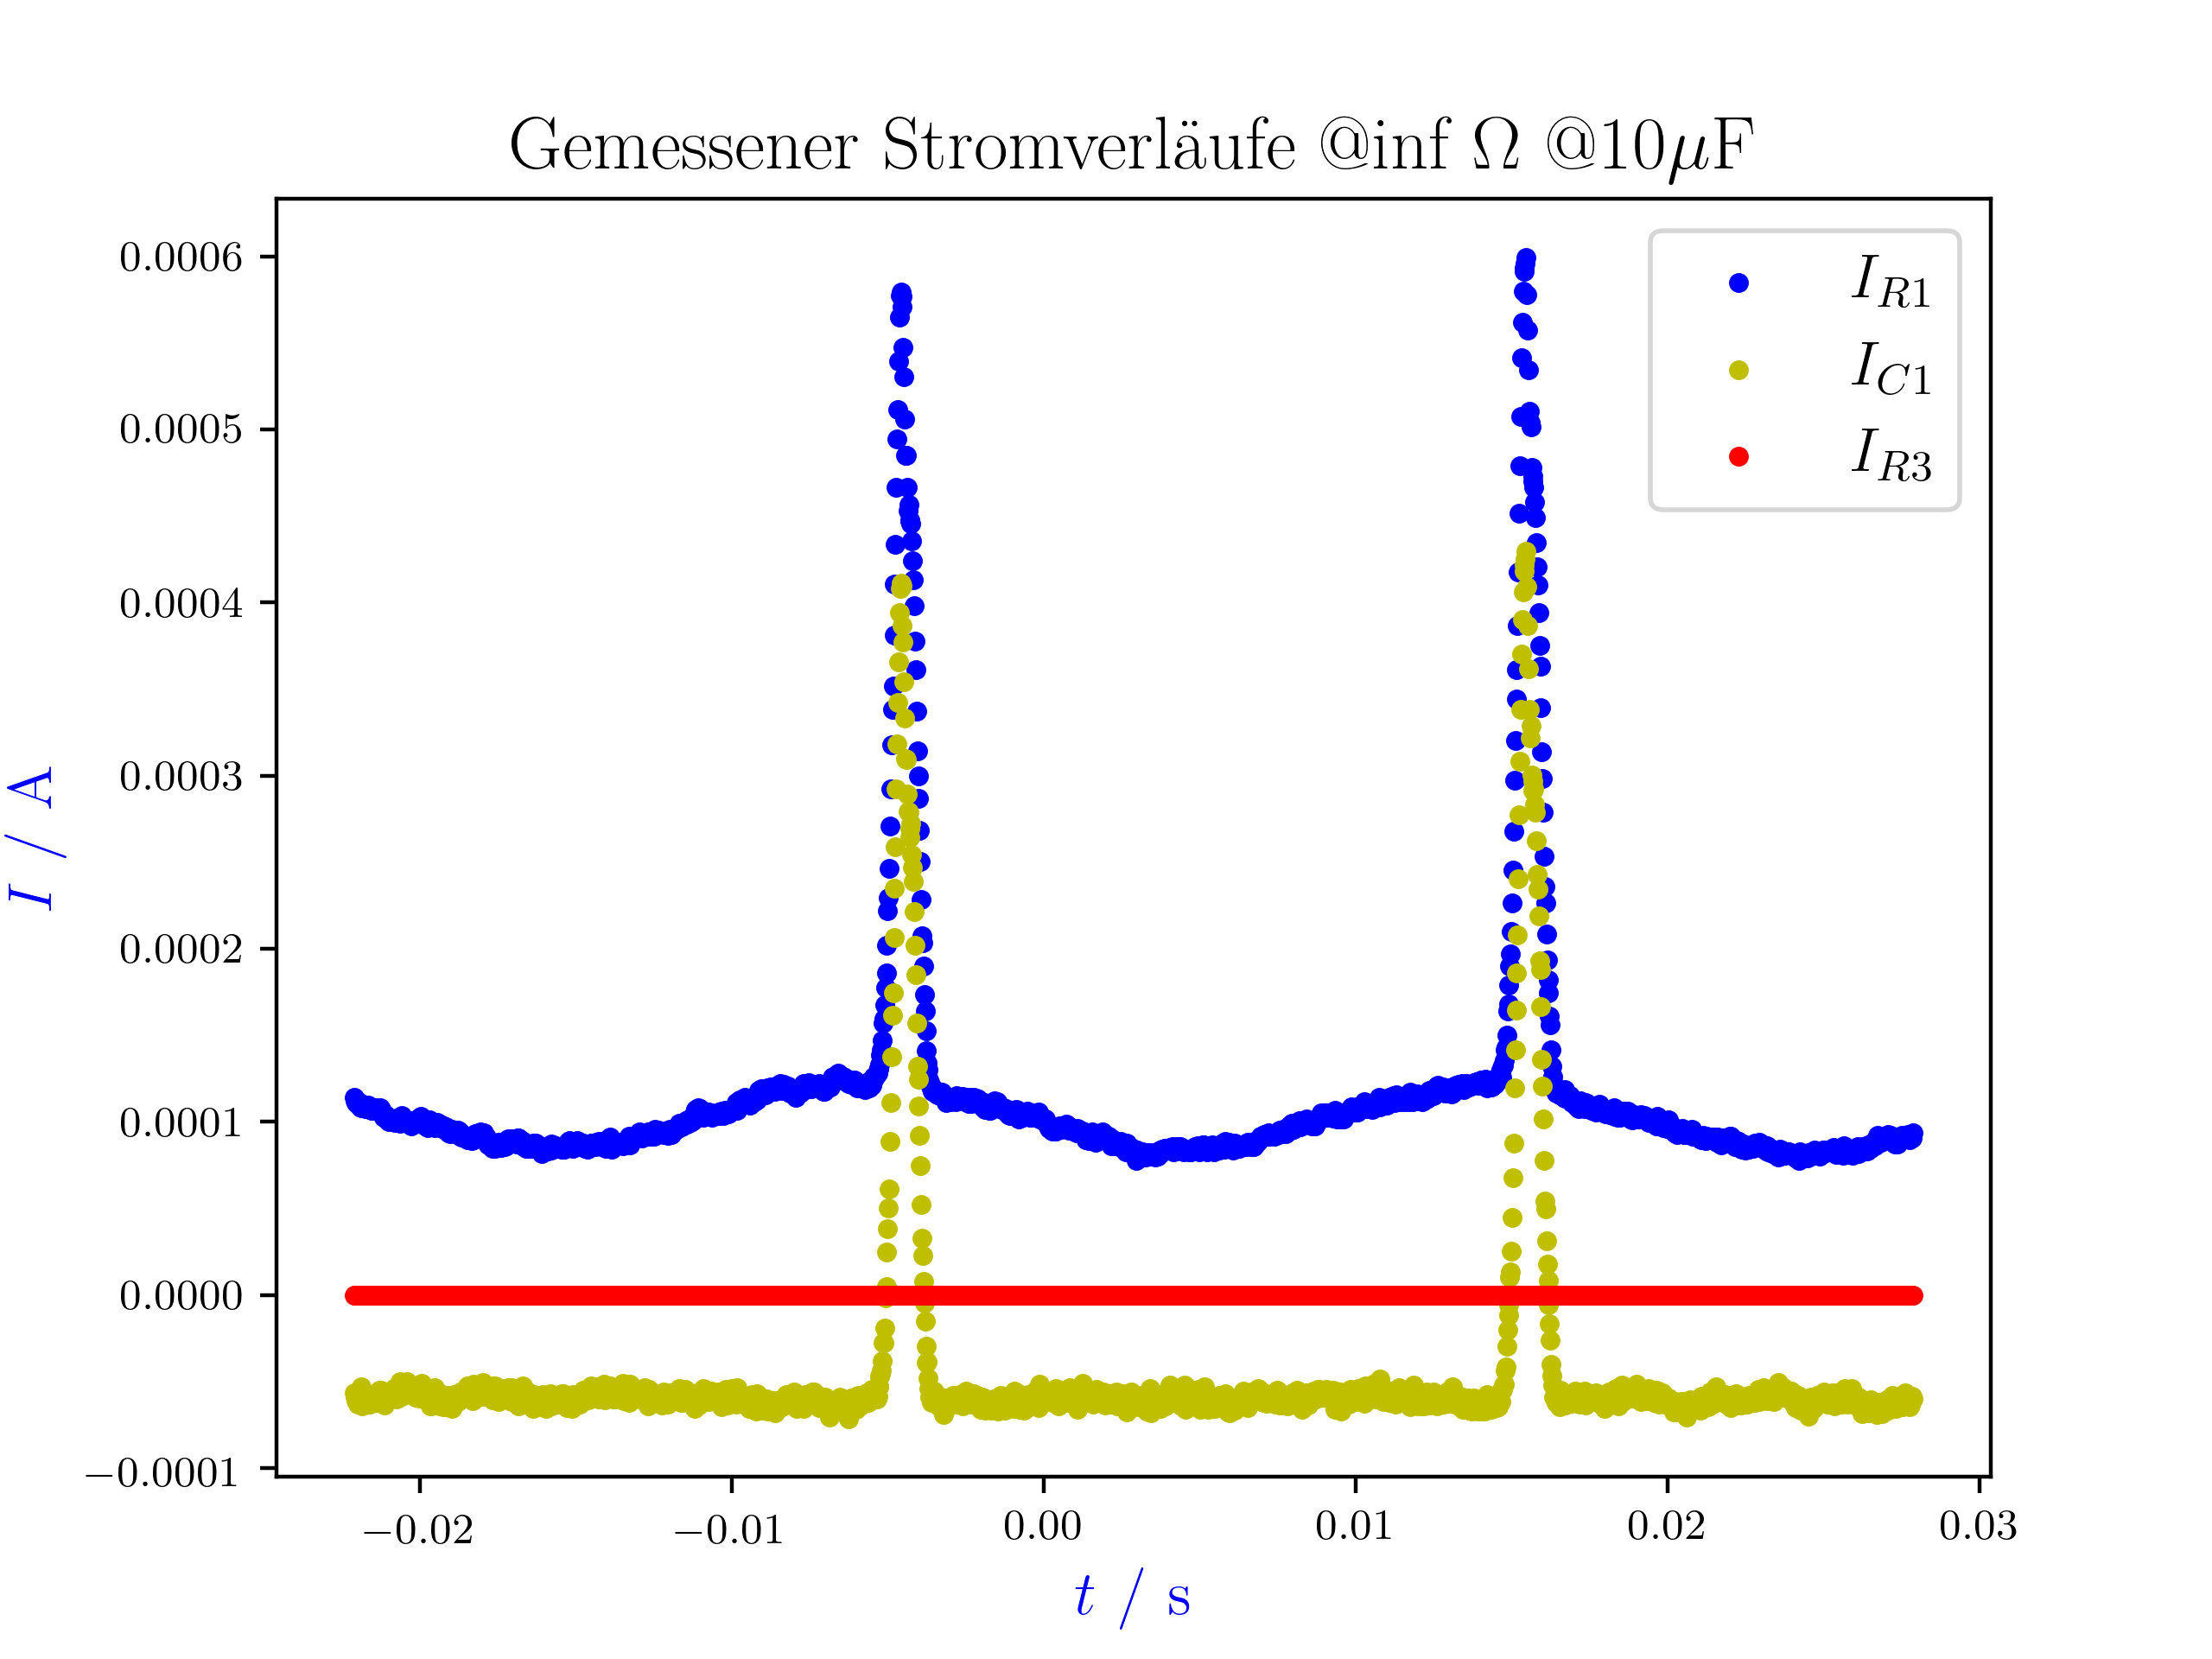
\includegraphics[width=\textwidth]{./figures/halbleiter/Versuch3/strominf.png}
		\captionof{figure}{Erhaltene Ströme bei einem Kondensator mit einer Kapazität von 10 $\mu$ Farad und einem $\infty$ großen Widerstand}
		\label{fig:strominf}
	\end{minipage}
\end{center}

\begin{center}
	\begin{minipage}[t]{0.8\textwidth}
		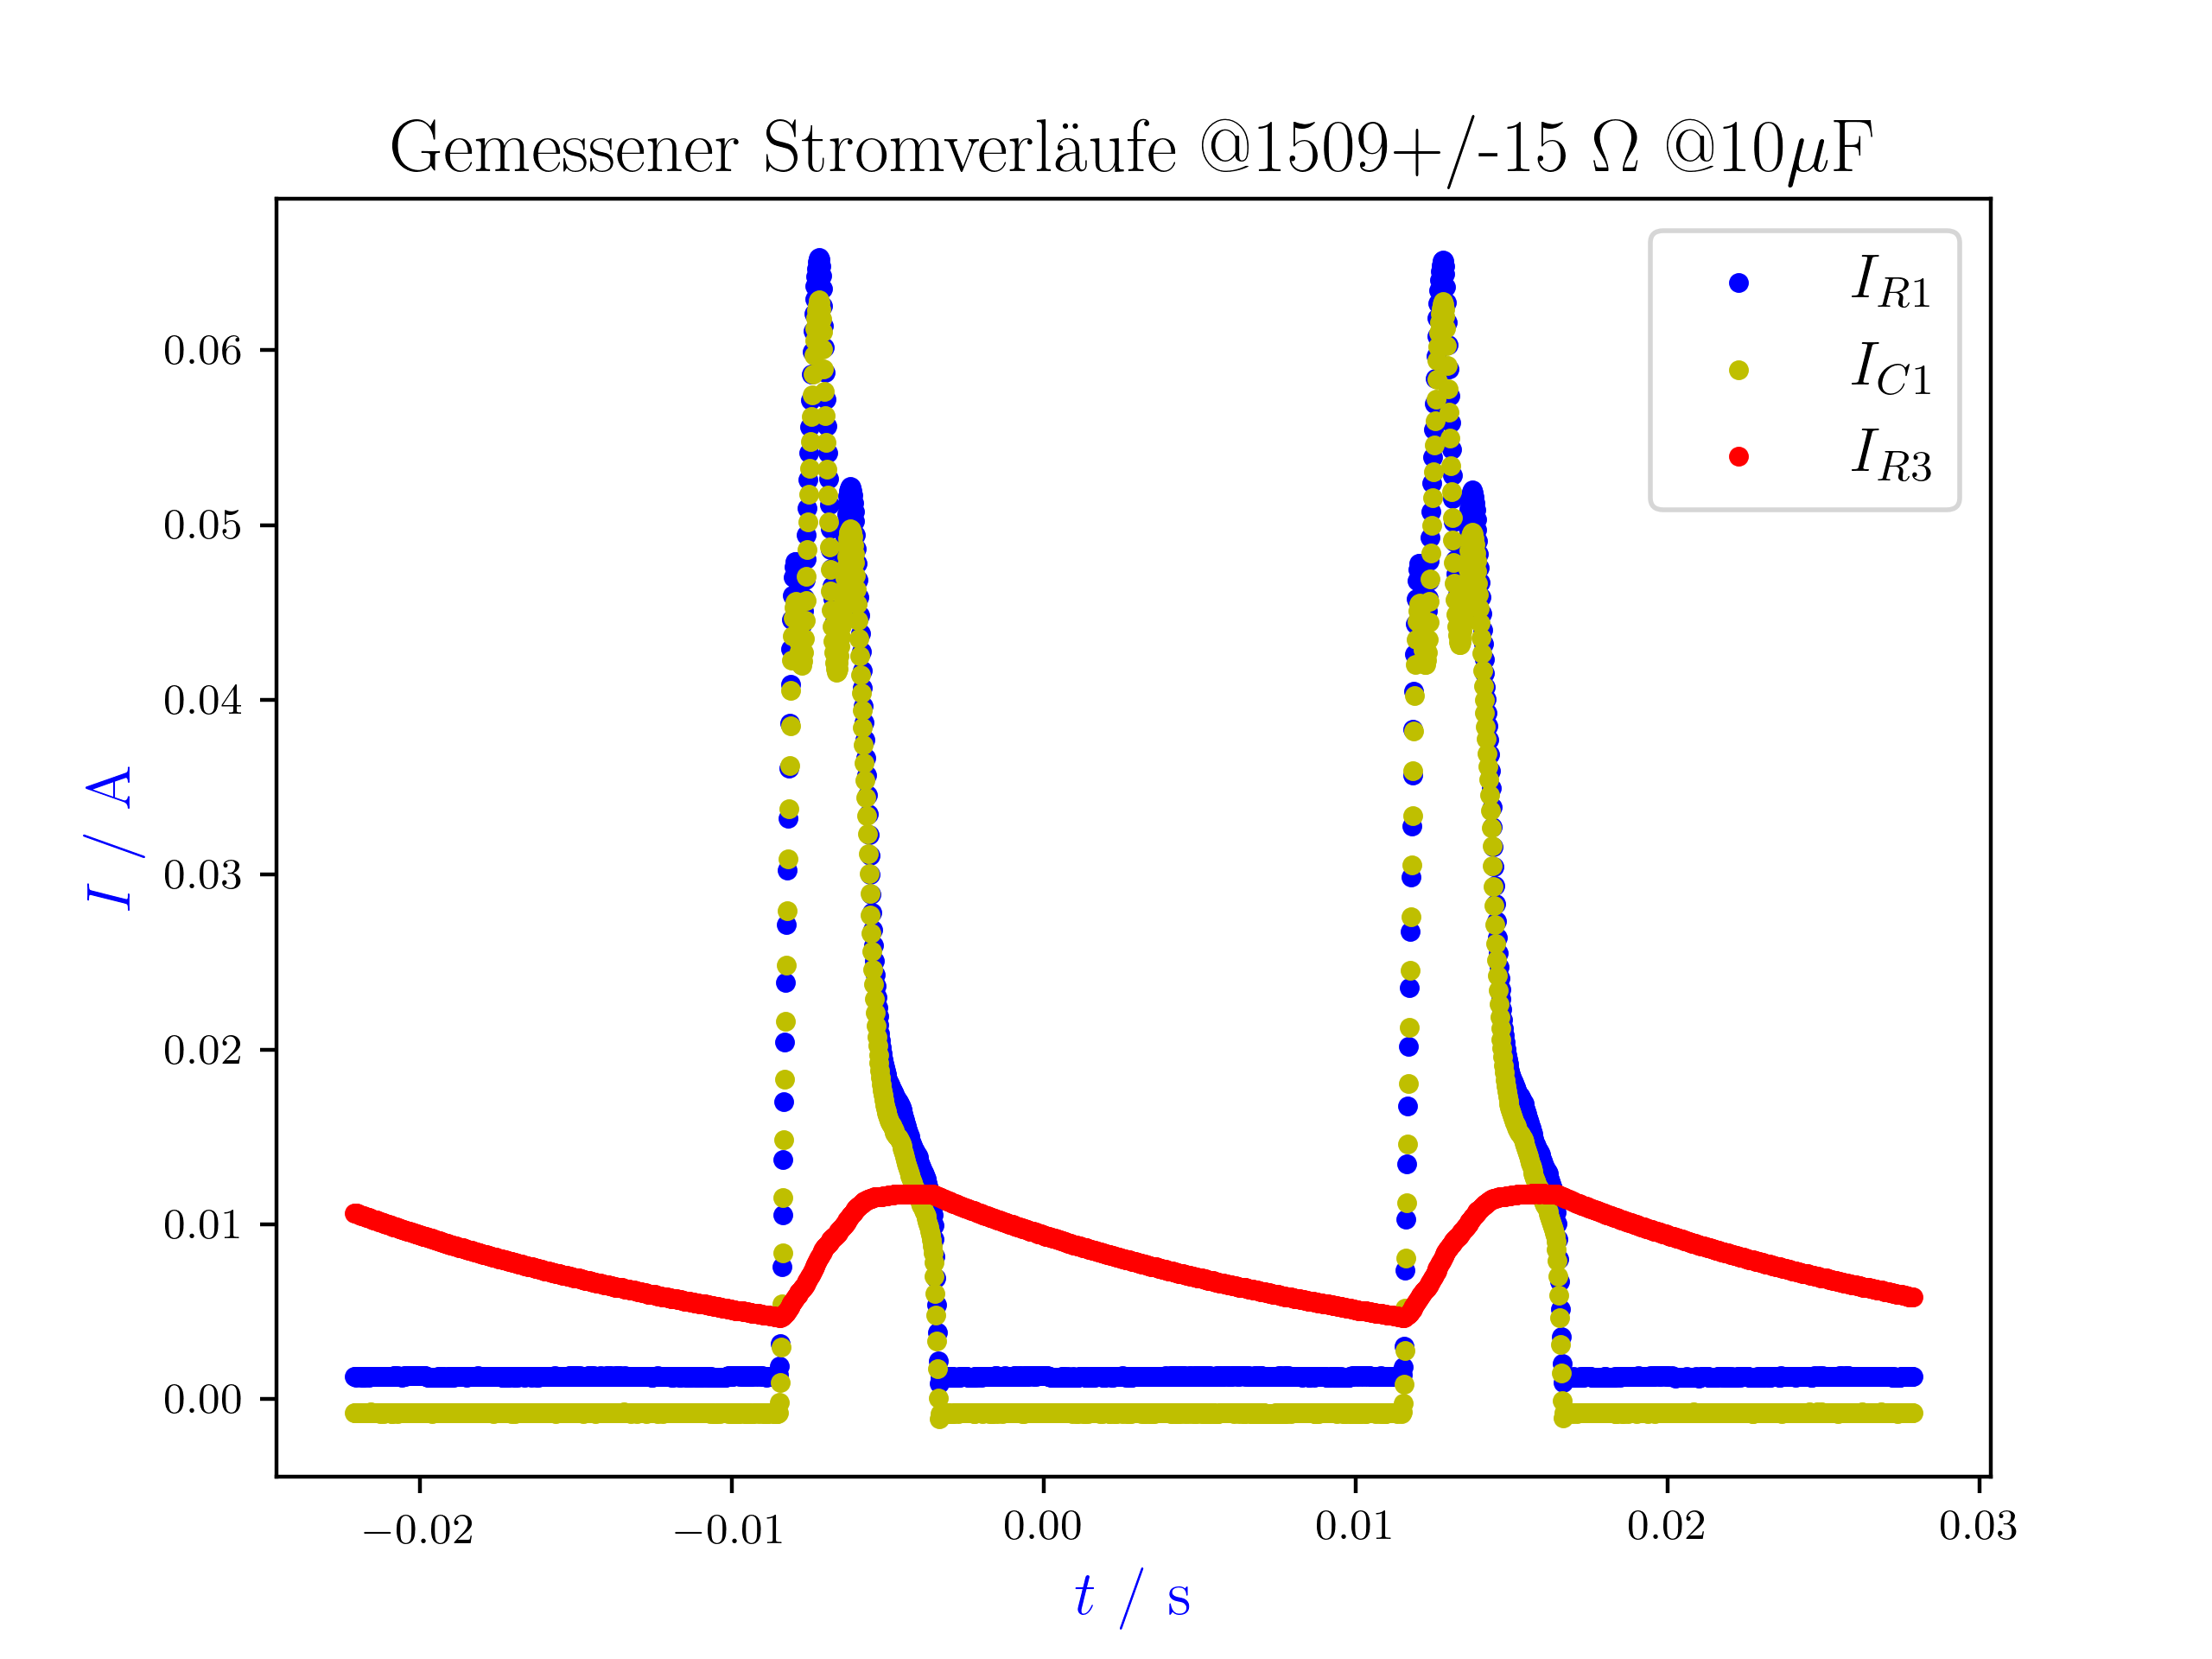
\includegraphics[width=\textwidth]{./figures/halbleiter/Versuch3/strom1509.0.png}
		\captionof{figure}{Erhaltene Ströme bei einem Kondensator mit einer Kapazität von 10 $\mu$ Farad und einem Widerstand von \SI{1509(15)}{} $\Omega$}
		\label{fig:strom1509}
	\end{minipage}
\end{center}


\begin{center}
	\begin{minipage}[t]{0.8\textwidth}
		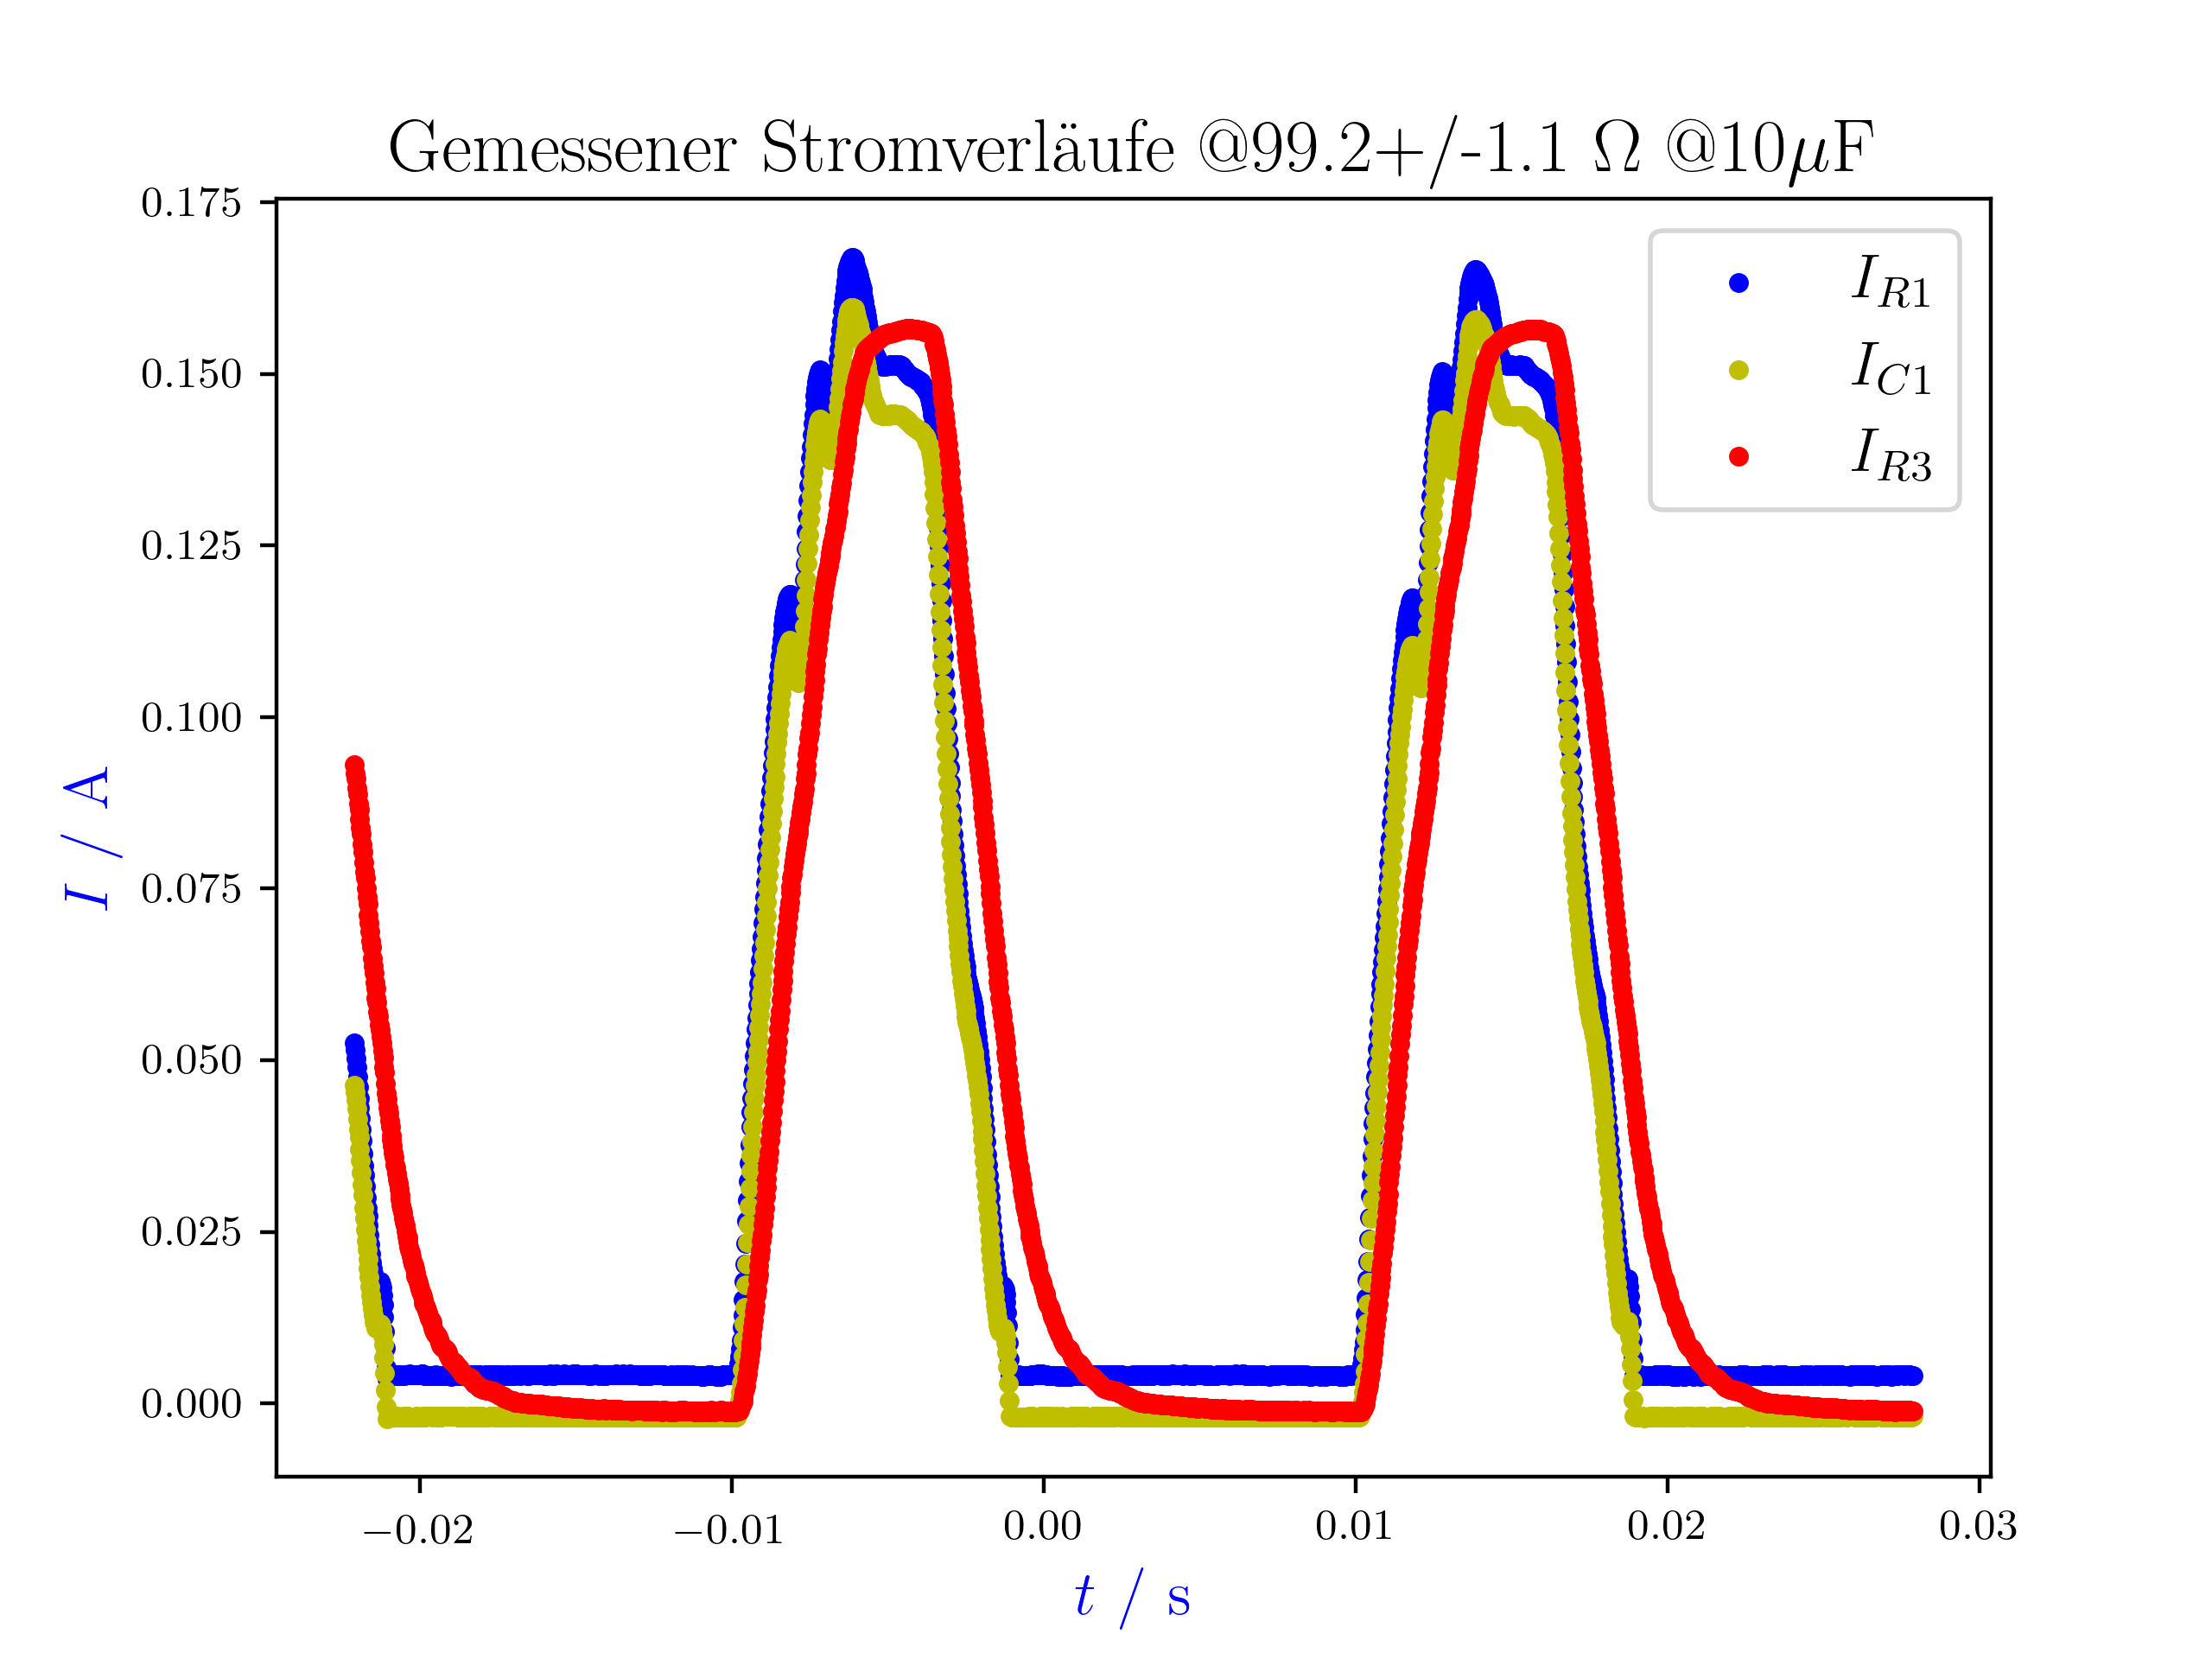
\includegraphics[width=\textwidth]{./figures/halbleiter/Versuch3/strom99.2.png}
		\captionof{figure}{Erhaltene Ströme bei einem Kondensator mit einer Kapazität von 10 $\mu$ Farad und einem Widerstand von \SI{99.2(11)}{\ohm}}
		\label{fig:strom100}
	\end{minipage}
\end{center}

Damit der Unterschied eines Größeren Kondensators für Glättung der Spannung untersucht werden kann wird die selbe Prozedur nochmals mit einem größeren Kondensator durchgeführt.
Wie bereits erwähnt wurde hier nur die Welligkeit ausgewertet, was in folgenden
% geglätteten Spannungskurven sind in folgenden
Abbildungen ersichtlich ist.


\begin{center}
	\begin{minipage}[t]{0.8\textwidth}
		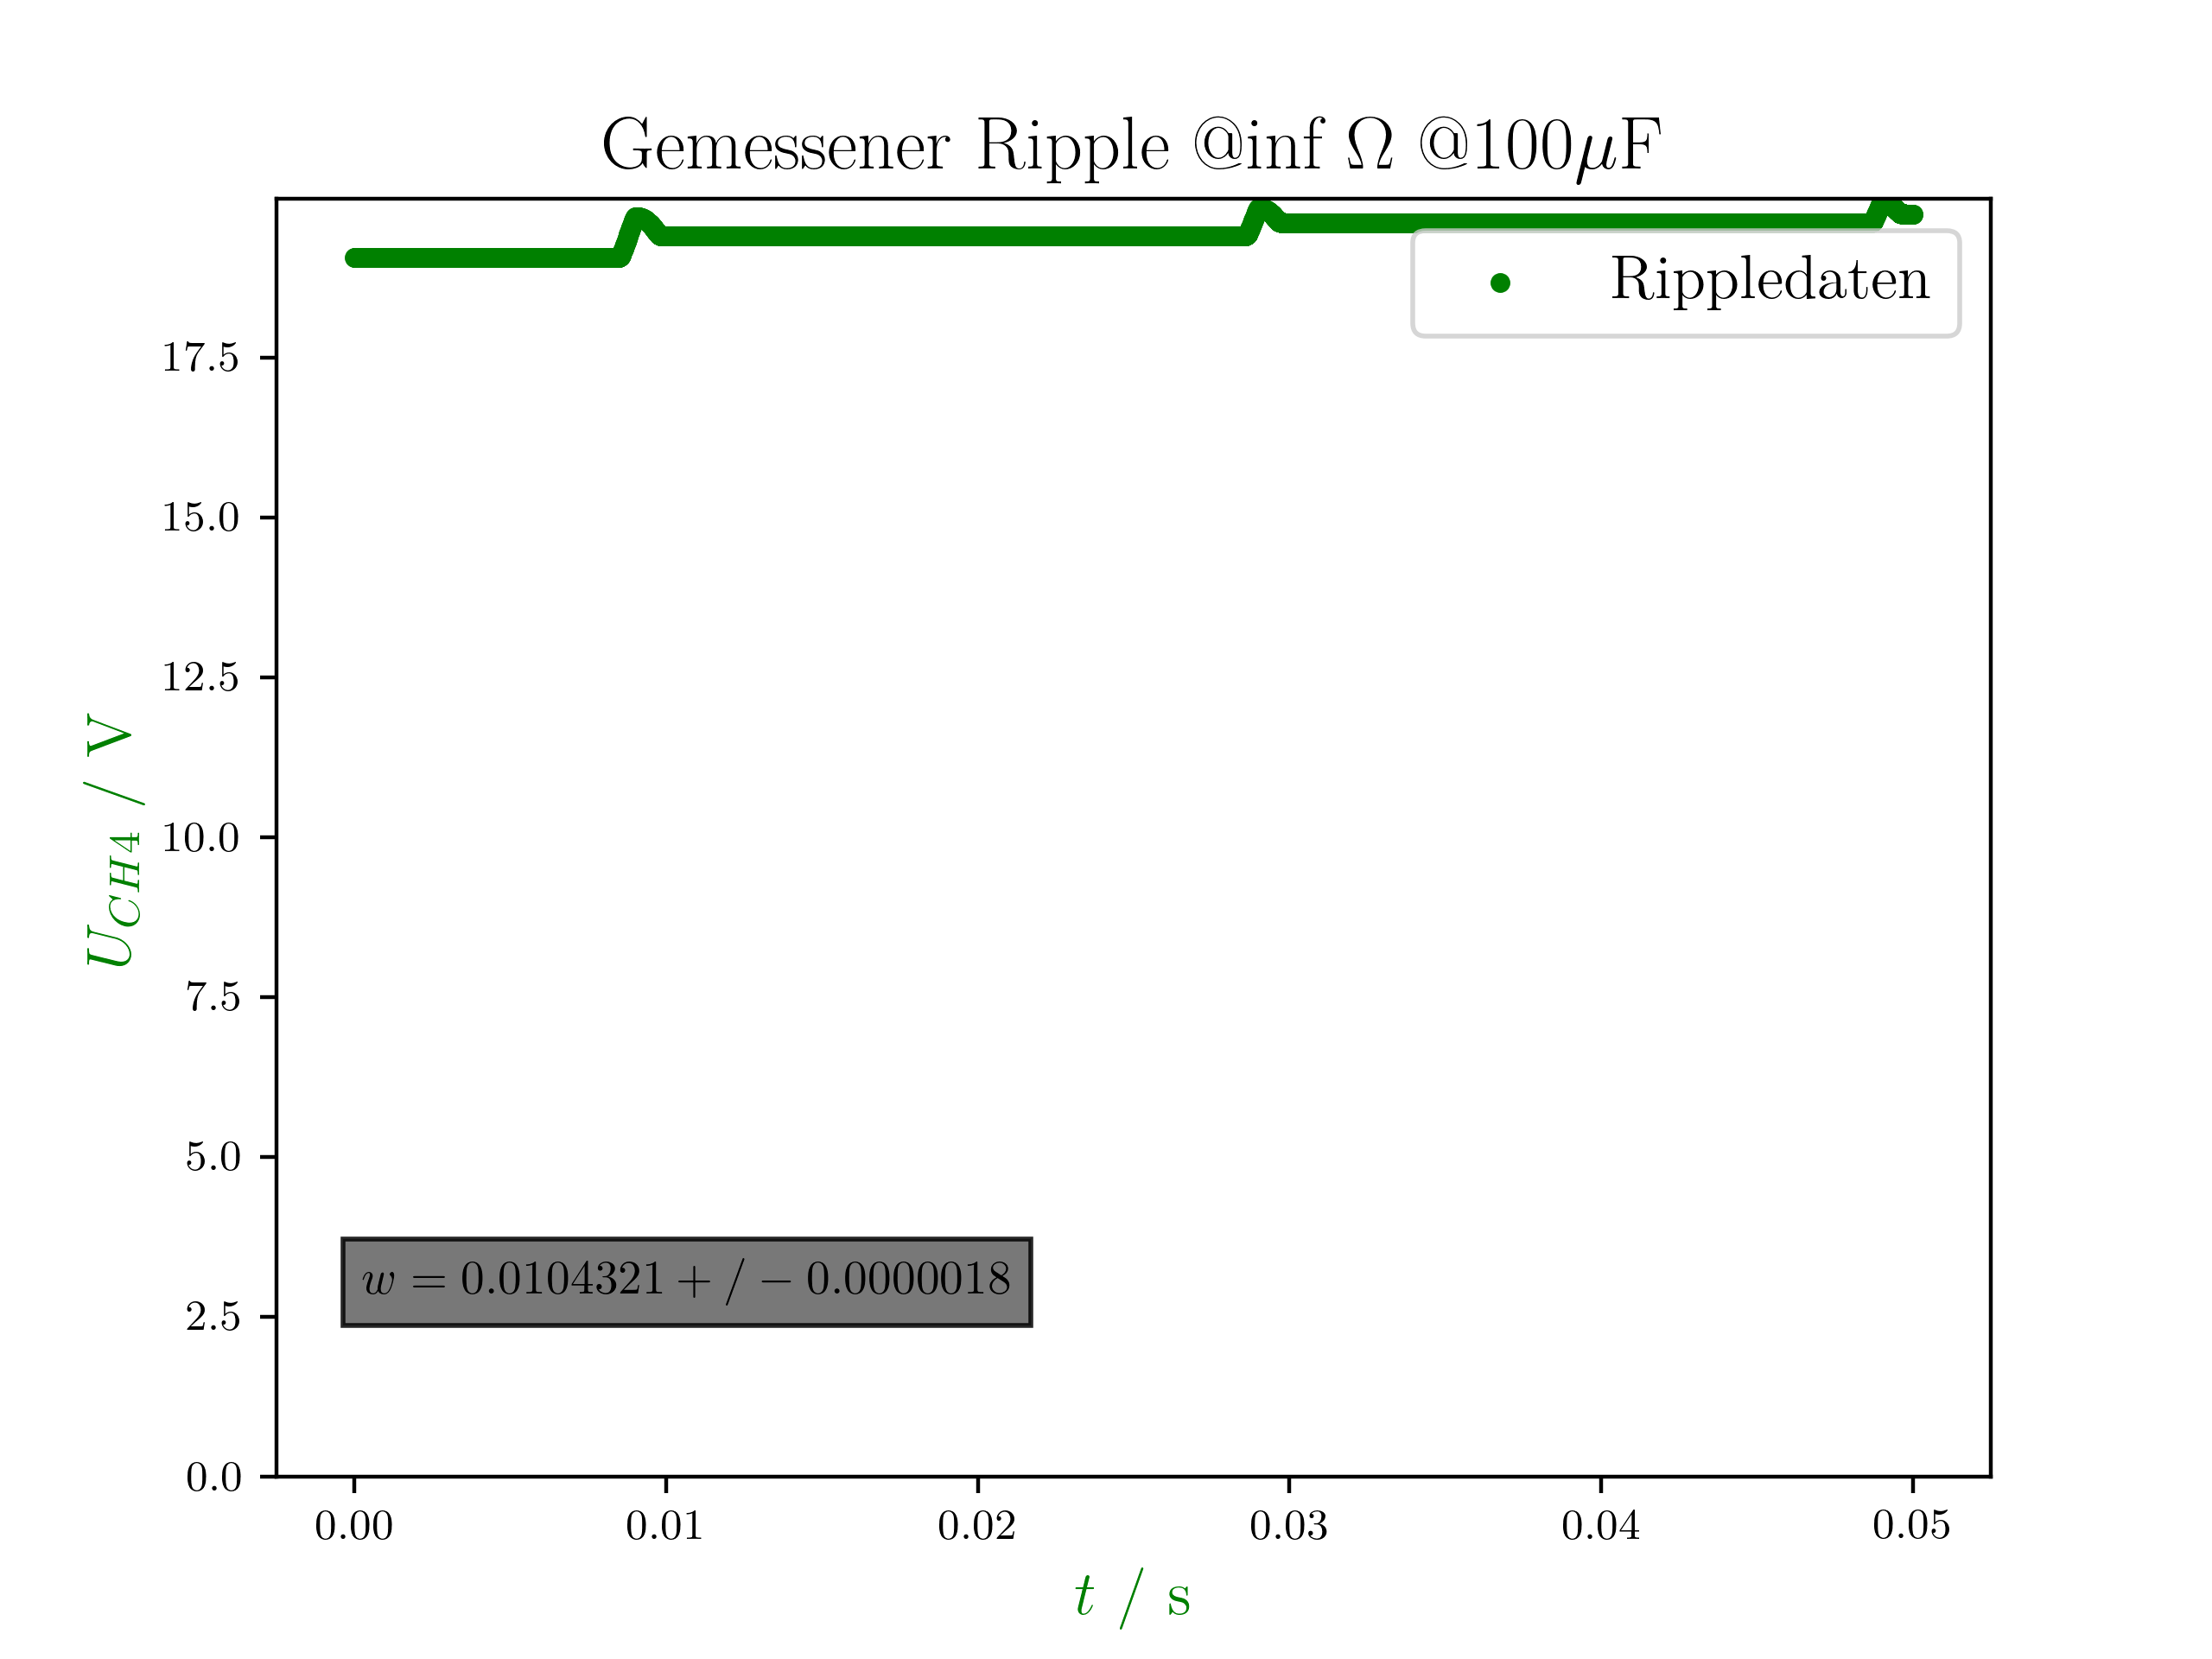
\includegraphics[width=\textwidth]{./figures/halbleiter/Versuch3/spannung_ripple_inf.png}
		\captionof{figure}{Geglätete Spannungskurve bei einem Kondensator mit einer Kapazität von 100 $\mu$ Farad und einem $\infty$ großen Widerstand}
		\label{fig:spannung_ripple_inf}
	\end{minipage}
\end{center}

\begin{center}
	\begin{minipage}[t]{0.8\textwidth}
		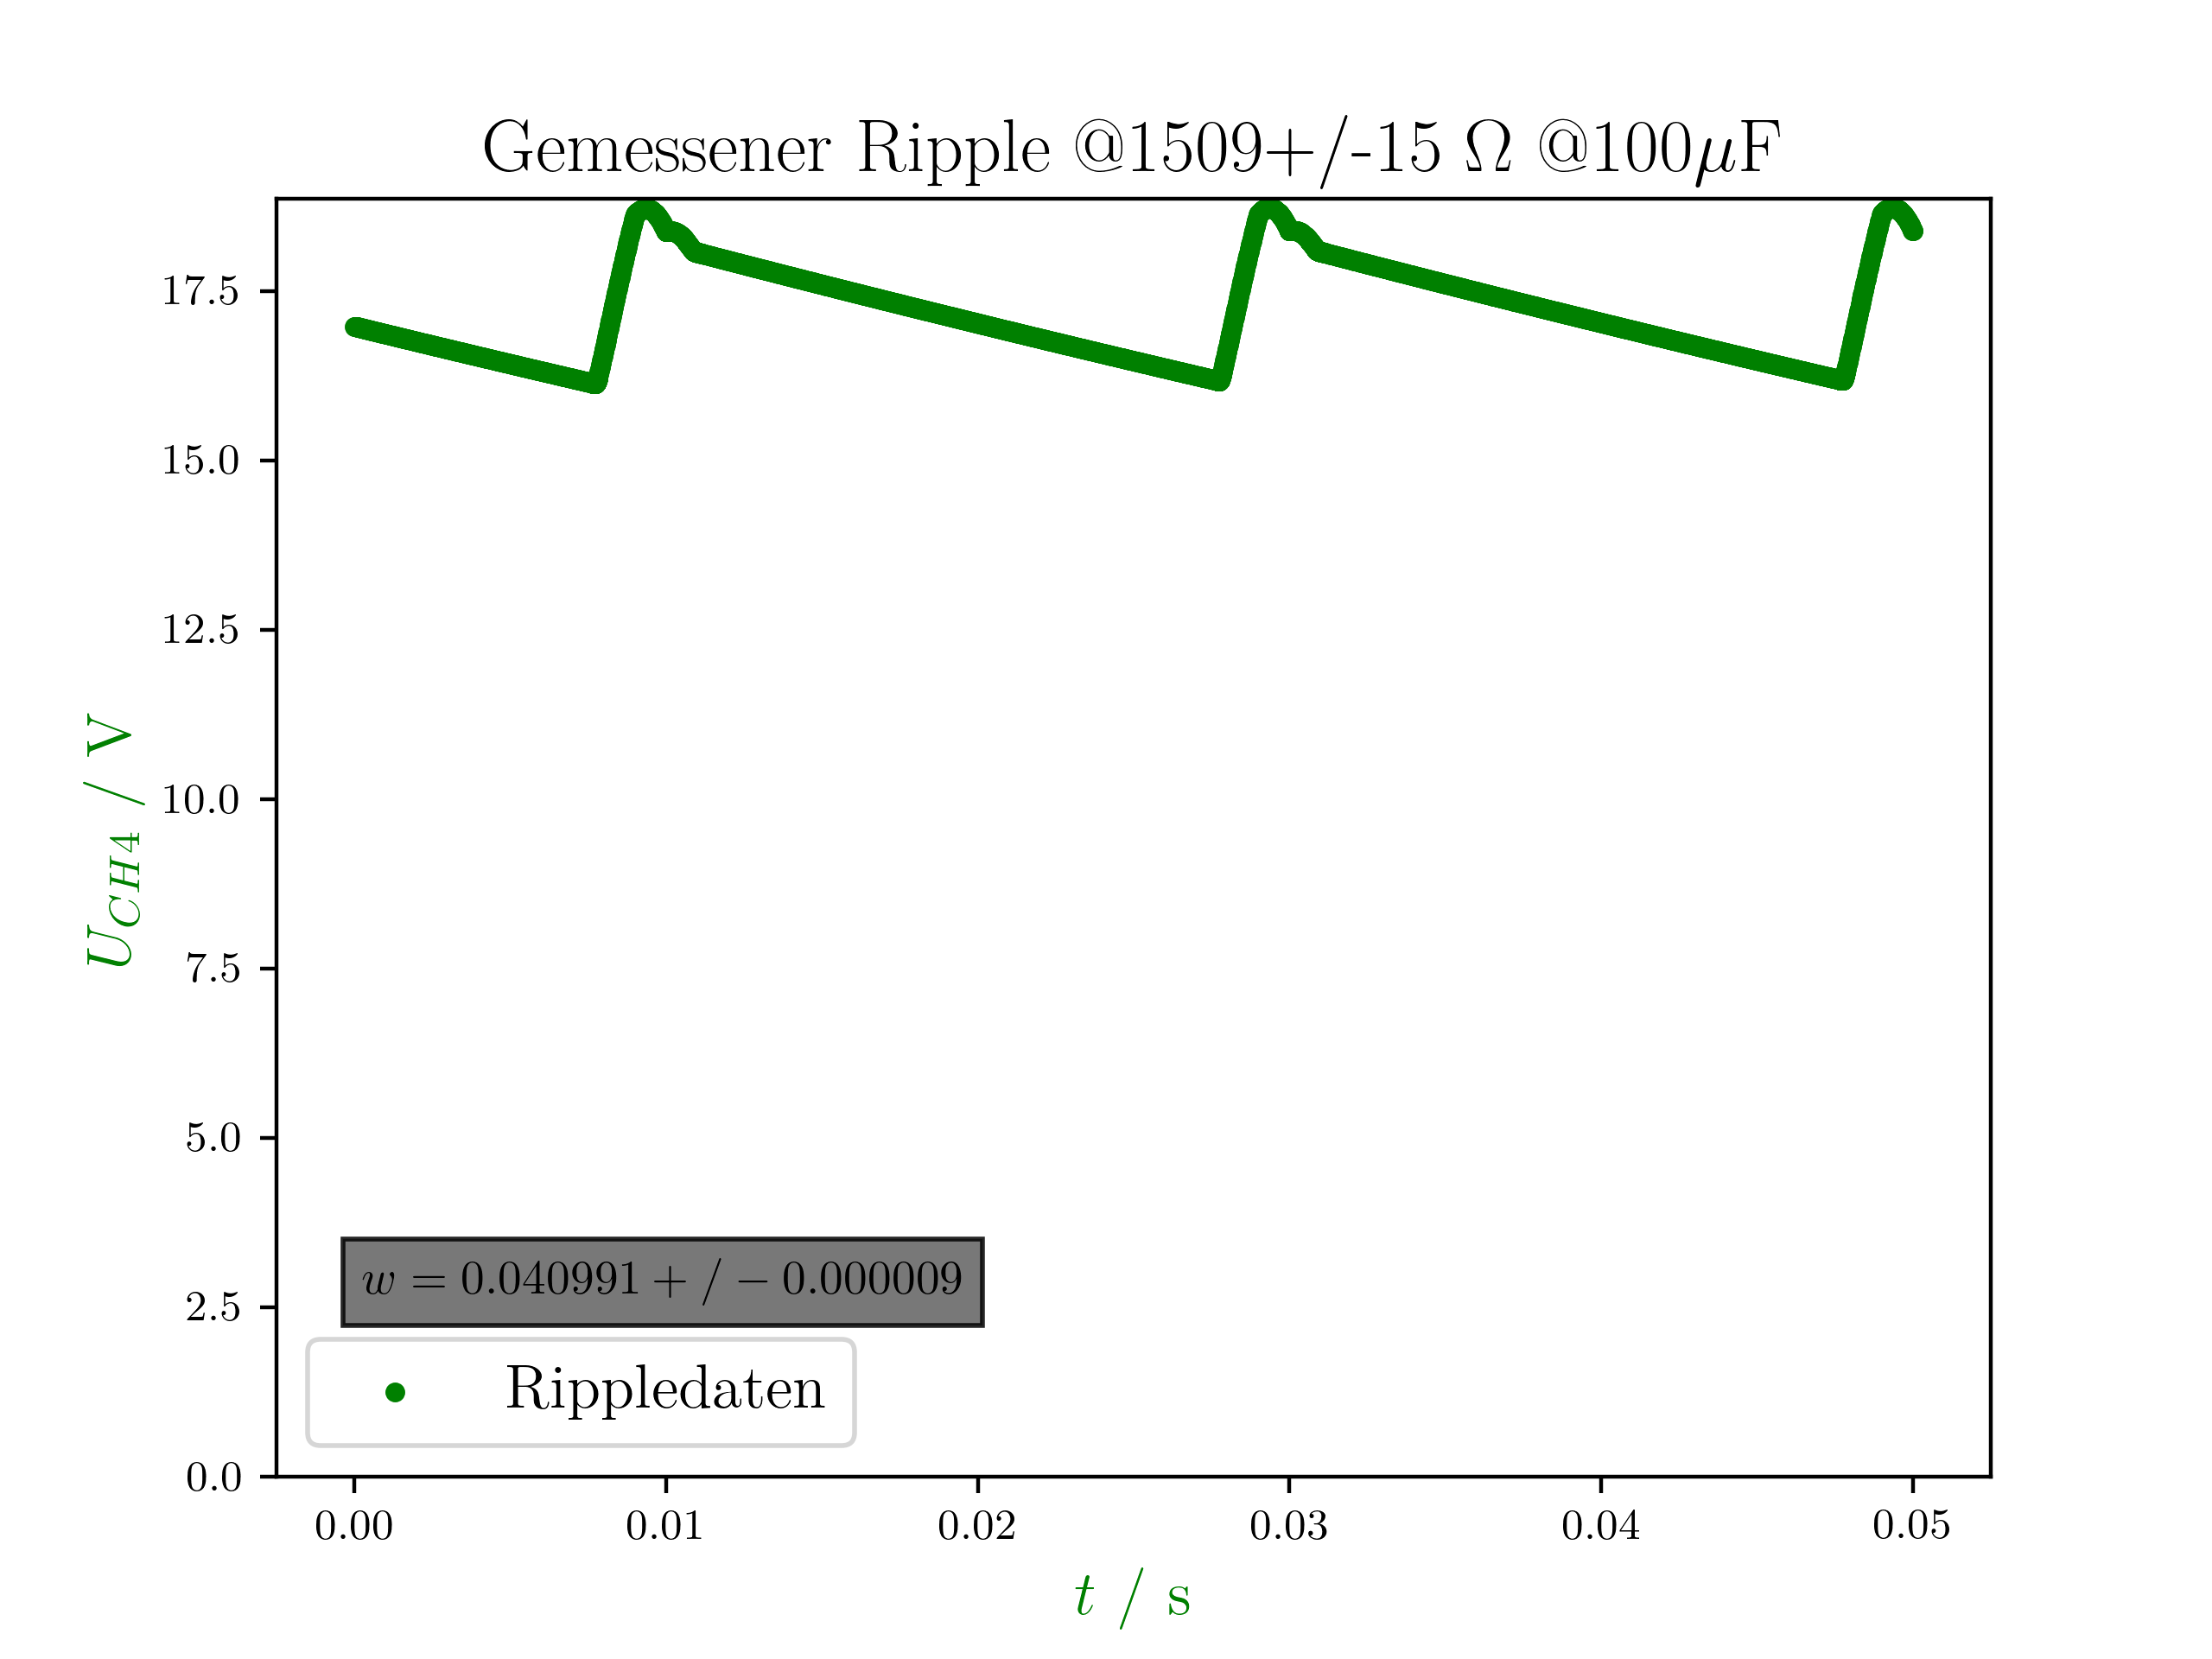
\includegraphics[width=\textwidth]{./figures/halbleiter/Versuch3/spannung_ripple_1509.0.png}
		\captionof{figure}{Geglätete Spannungskurve bei einem Kondensator mit einer Kapazität von 100 $\mu$ Farad und einem Widerstand von \SI{1509(15)}{} $\Omega$}
		\label{fig:spannung_ripple_1509}
	\end{minipage}
\end{center}

\begin{center}
	\begin{minipage}[t]{0.8\textwidth}
		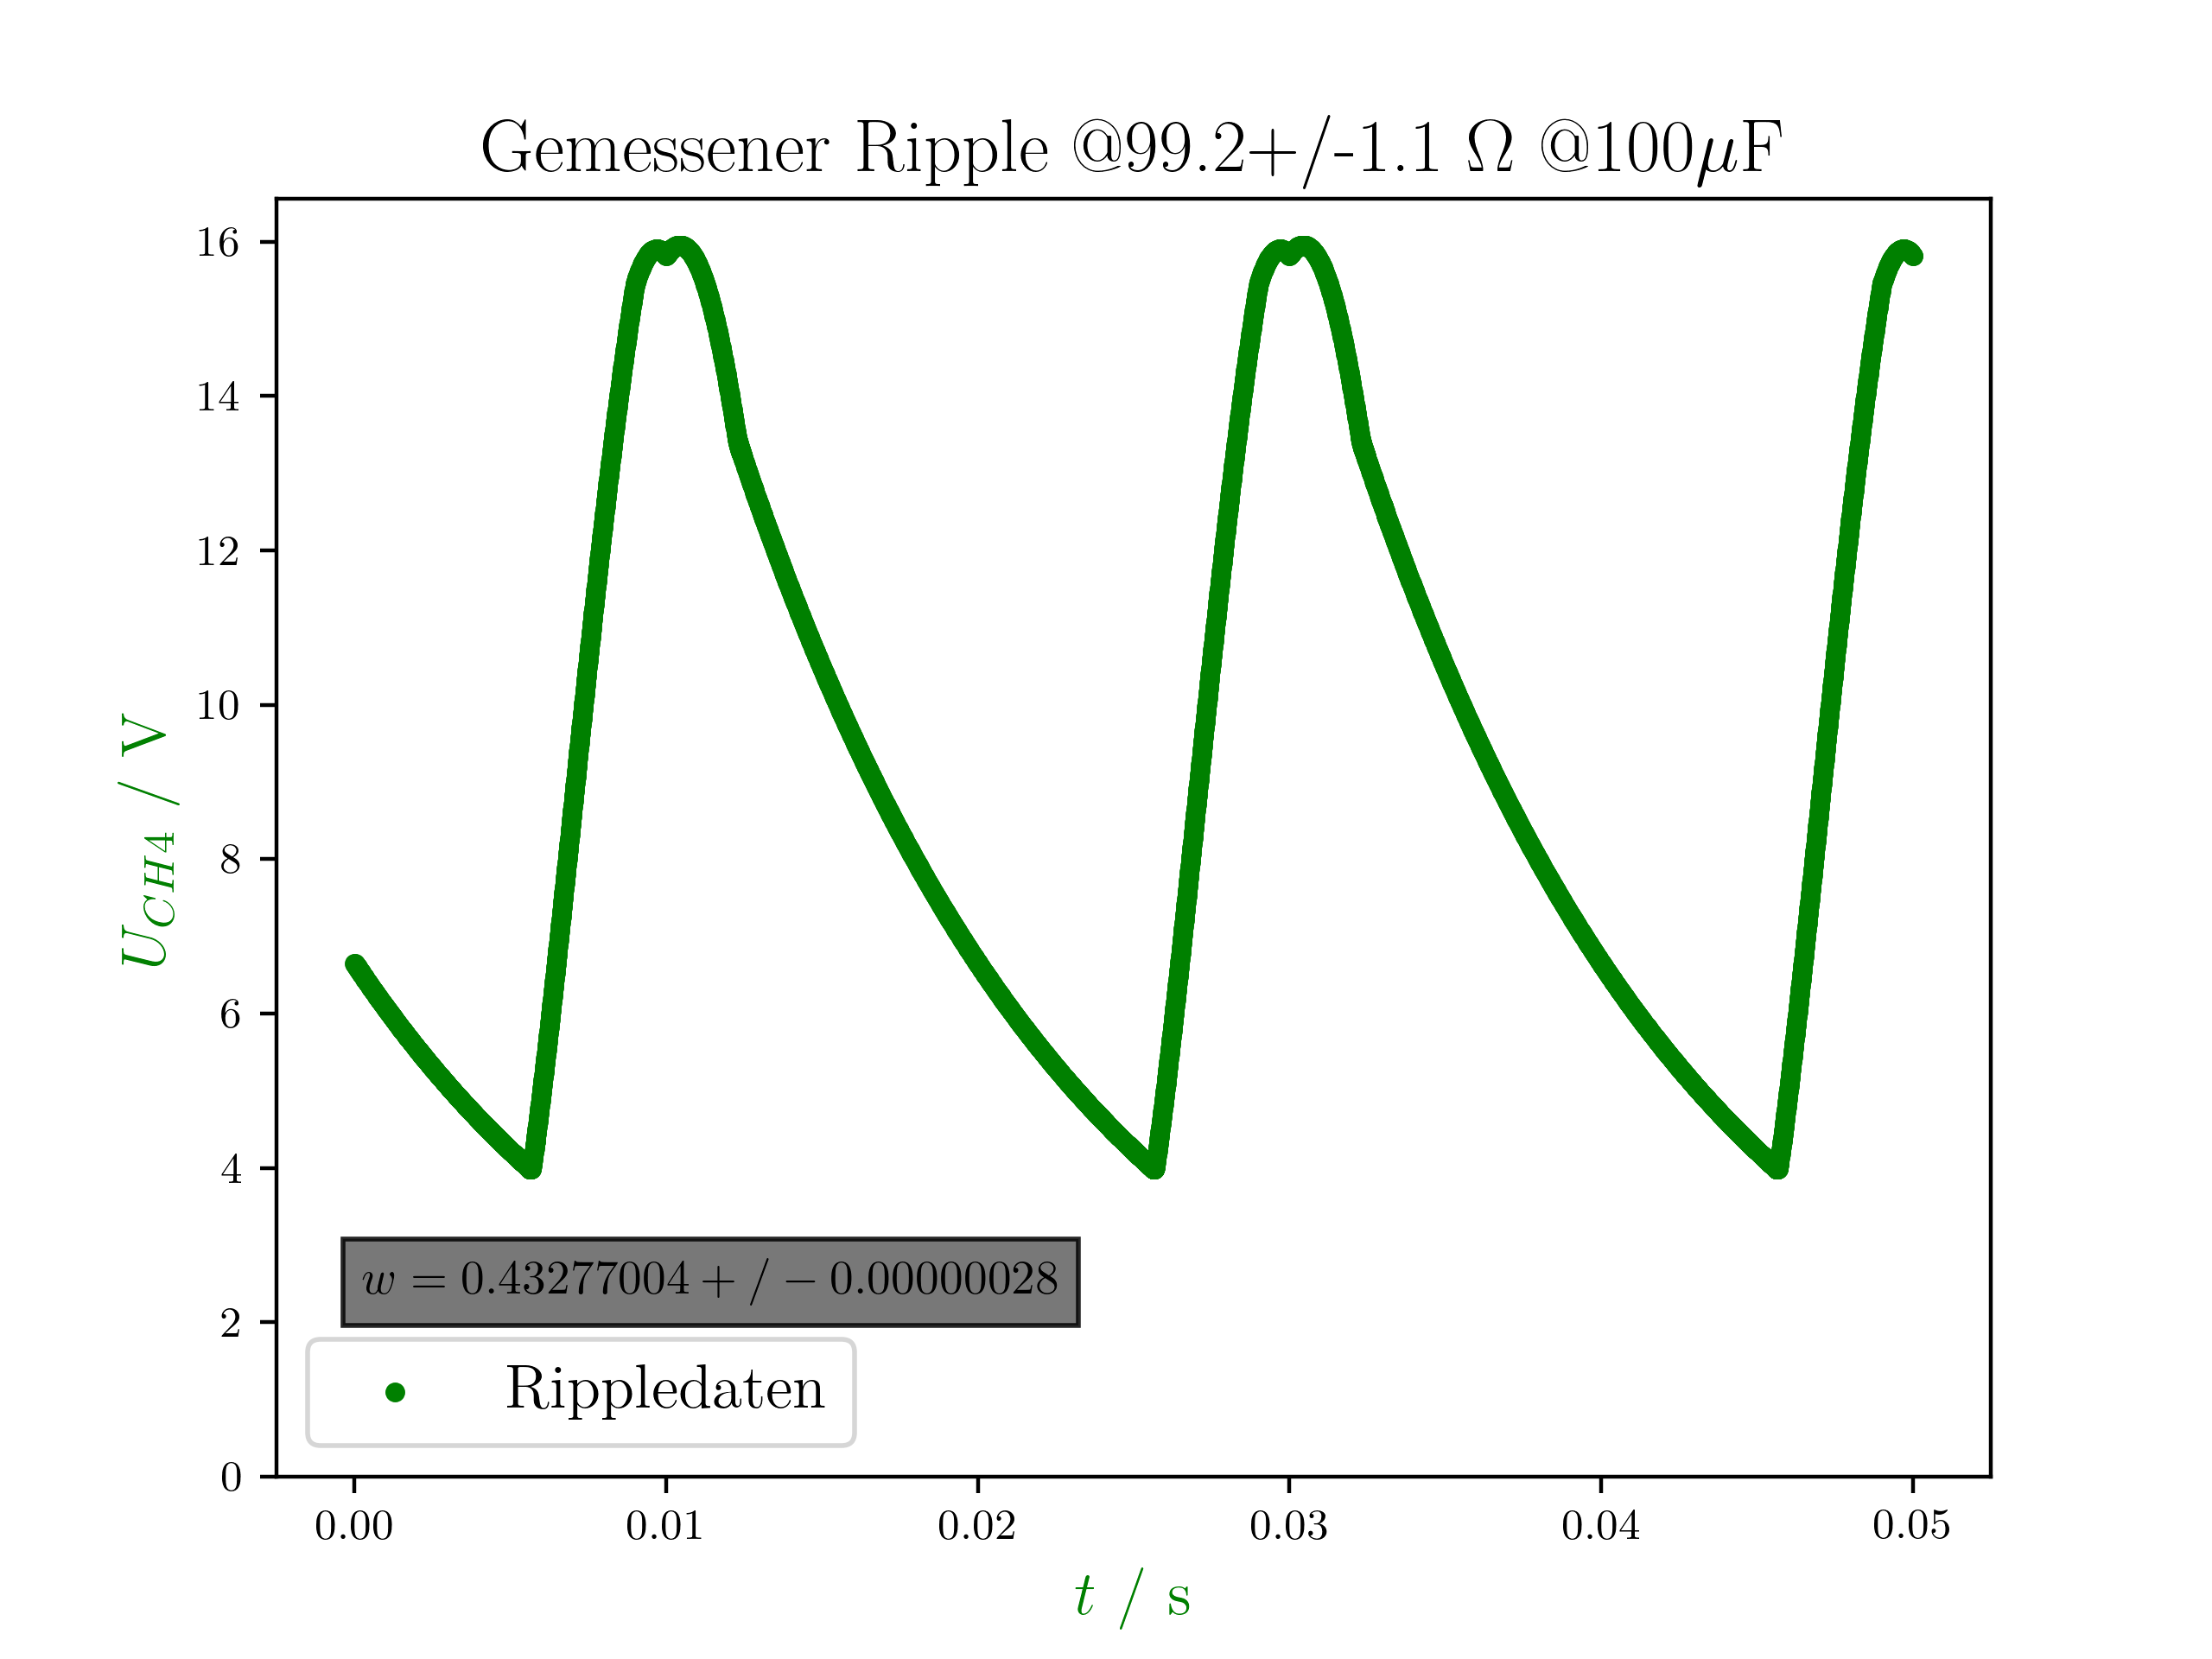
\includegraphics[width=\textwidth]{./figures/halbleiter/Versuch3/spannung_ripple_99.2.png}
		\captionof{figure}{Geglätete Spannungskurve bei einem Kondensator mit einer Kapazität von 100 $\mu$ Farad und einem Widerstand von \num{99.2(11)} $\Omega$}
		\label{fig:spannung_ripple_100}
	\end{minipage}
\end{center}

\vspace{5mm}

\subsection{Untersuchung der Spannungsverläufe in einer Spannungsverdopplerschaltung}

Zunächst wird die grafische Darstellung der Spannungsverläufe an den Bauteilen als Funktion der Zeit
über mehrere Perioden für beide Belastungsfälle veranschaulicht.

\vspace{2mm}

In den folgenden Abbildungen sind die aufgezeichneten Spannungsverläufe
mit, \autoref{fig:versuch4spannugenmit} und ohne,
\autoref{fig:versuch4spannugenohne}, Belastung ersichtlich.

\begin{center}
	\begin{minipage}[t]{0.8\textwidth}
		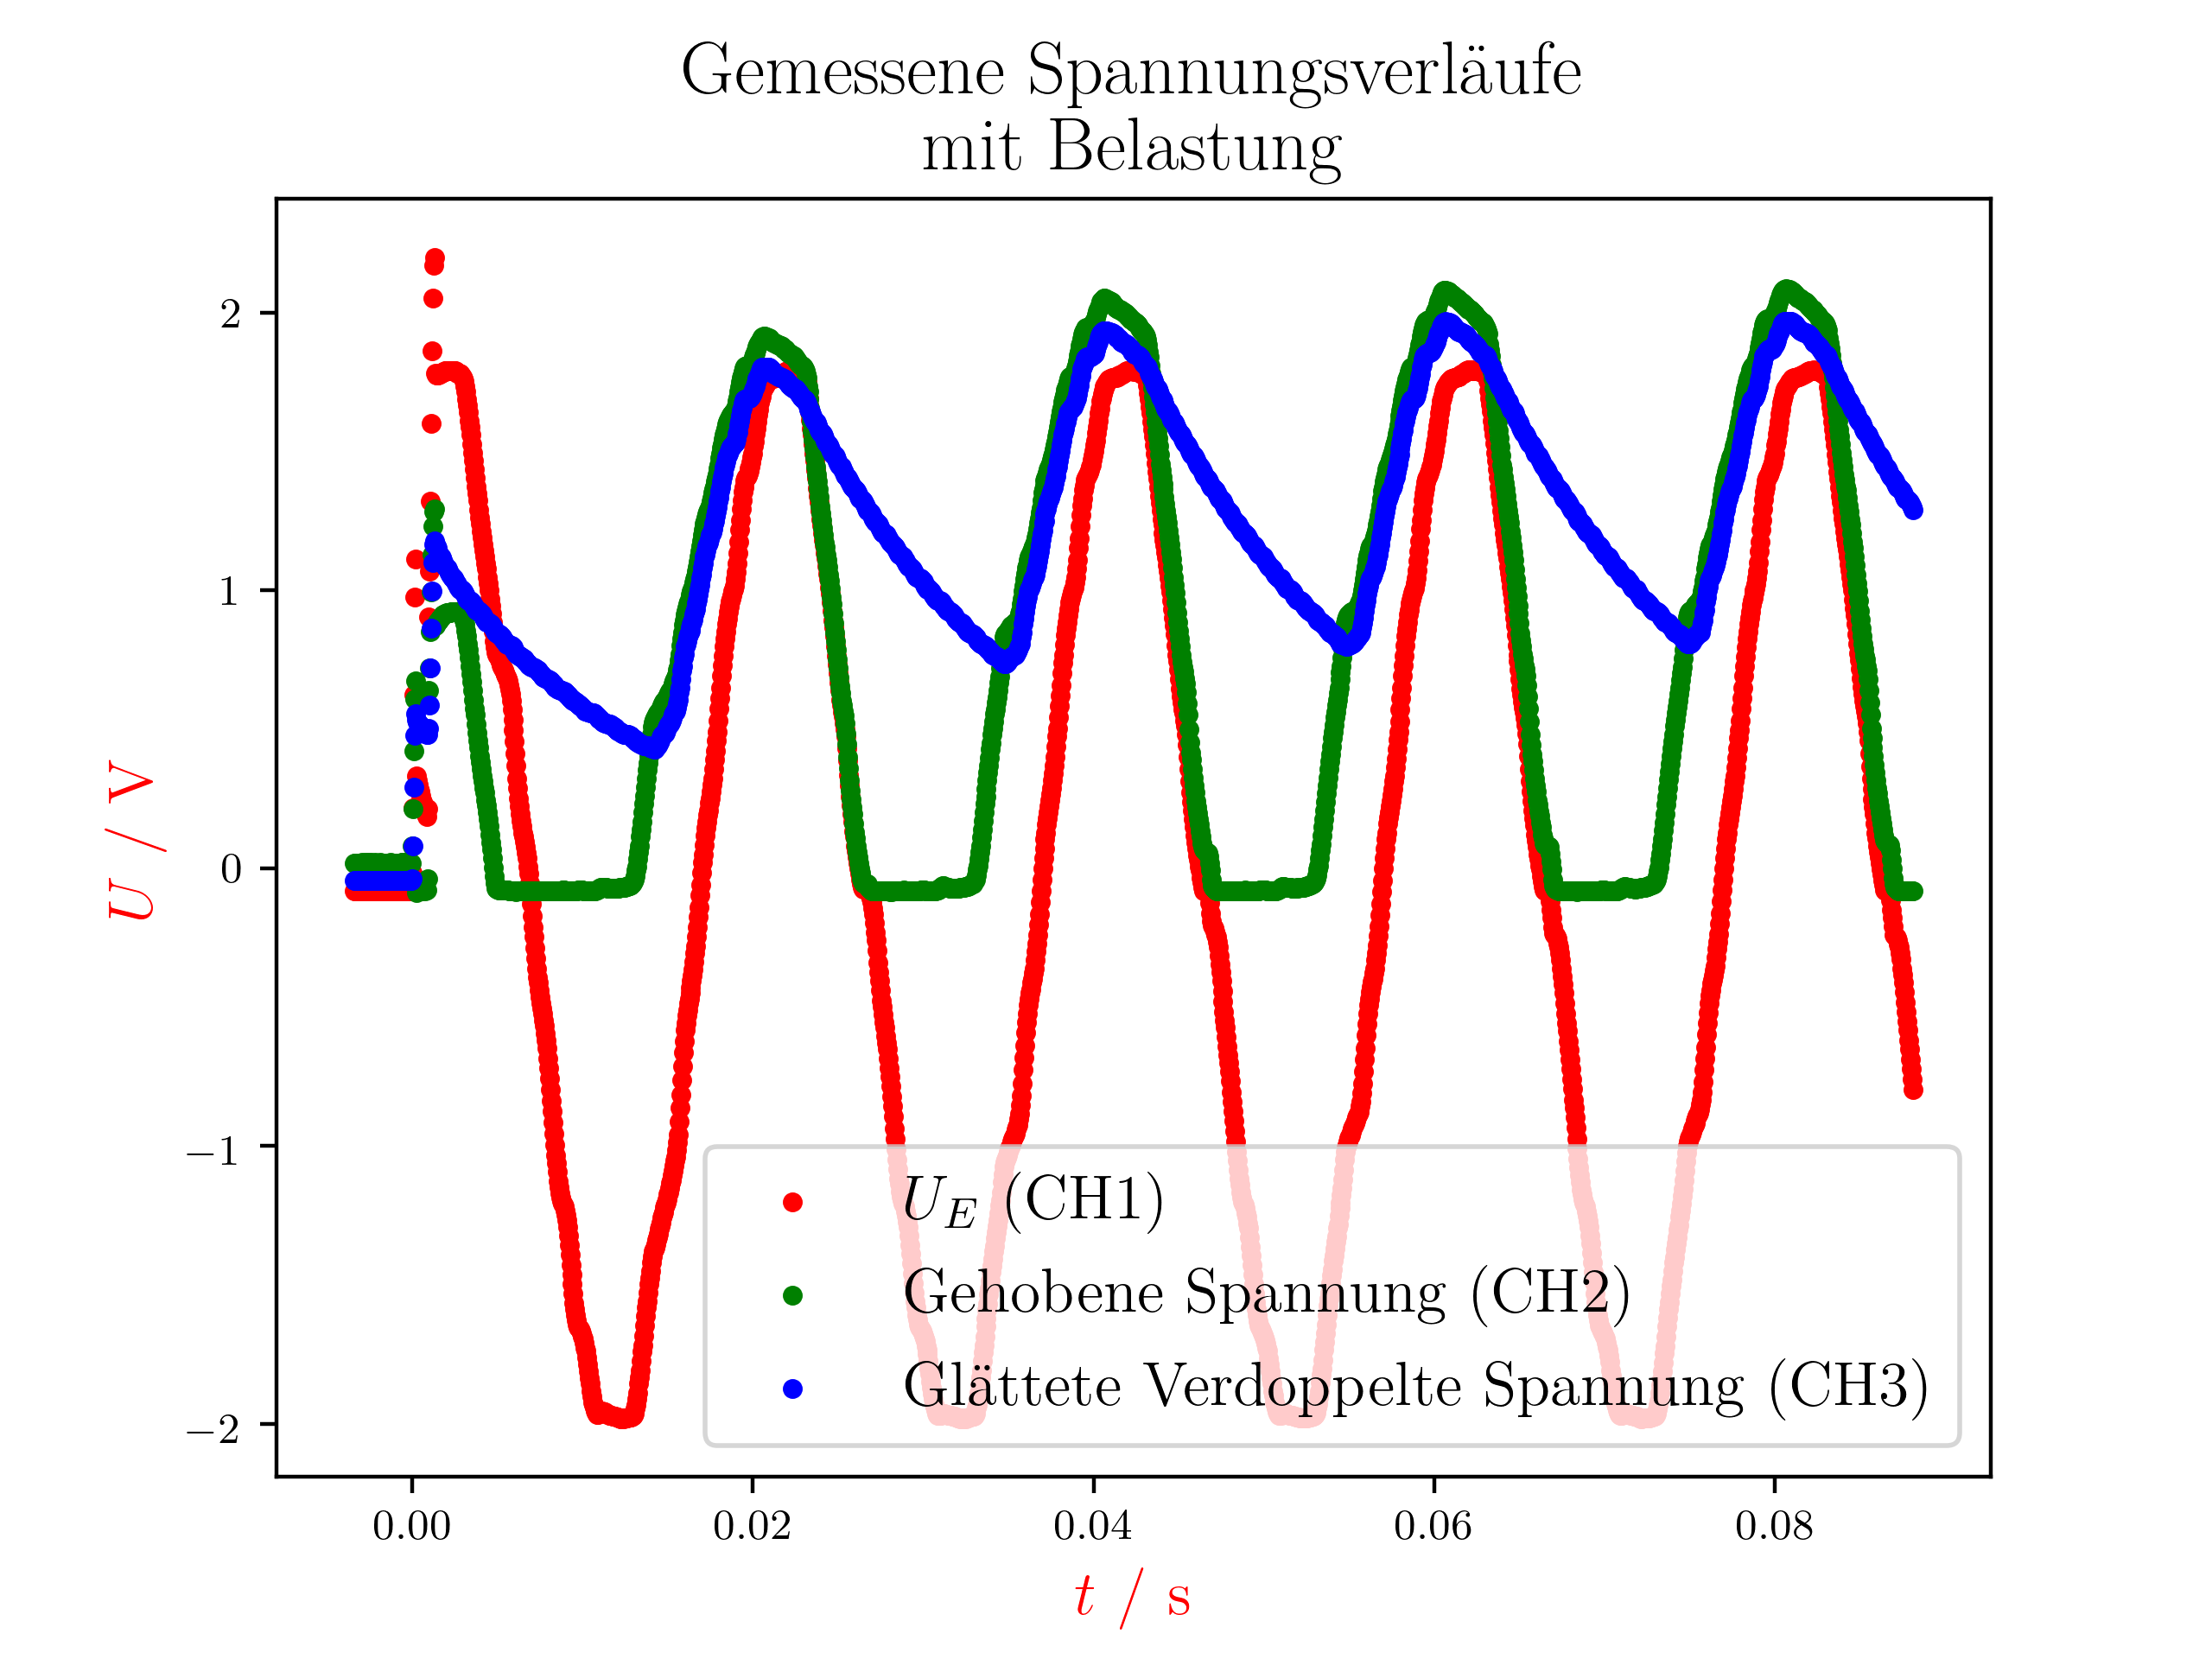
\includegraphics[width=\textwidth]{./figures/halbleiter/Versuch4/versuch4spannugenmit.png}
		\captionof{figure}{Gemessener Spannungsverlauf mit einer Belastung}
		\label{fig:versuch4spannugenmit}
	\end{minipage}
\end{center}

\begin{center}
	\begin{minipage}[t]{0.8\textwidth}
		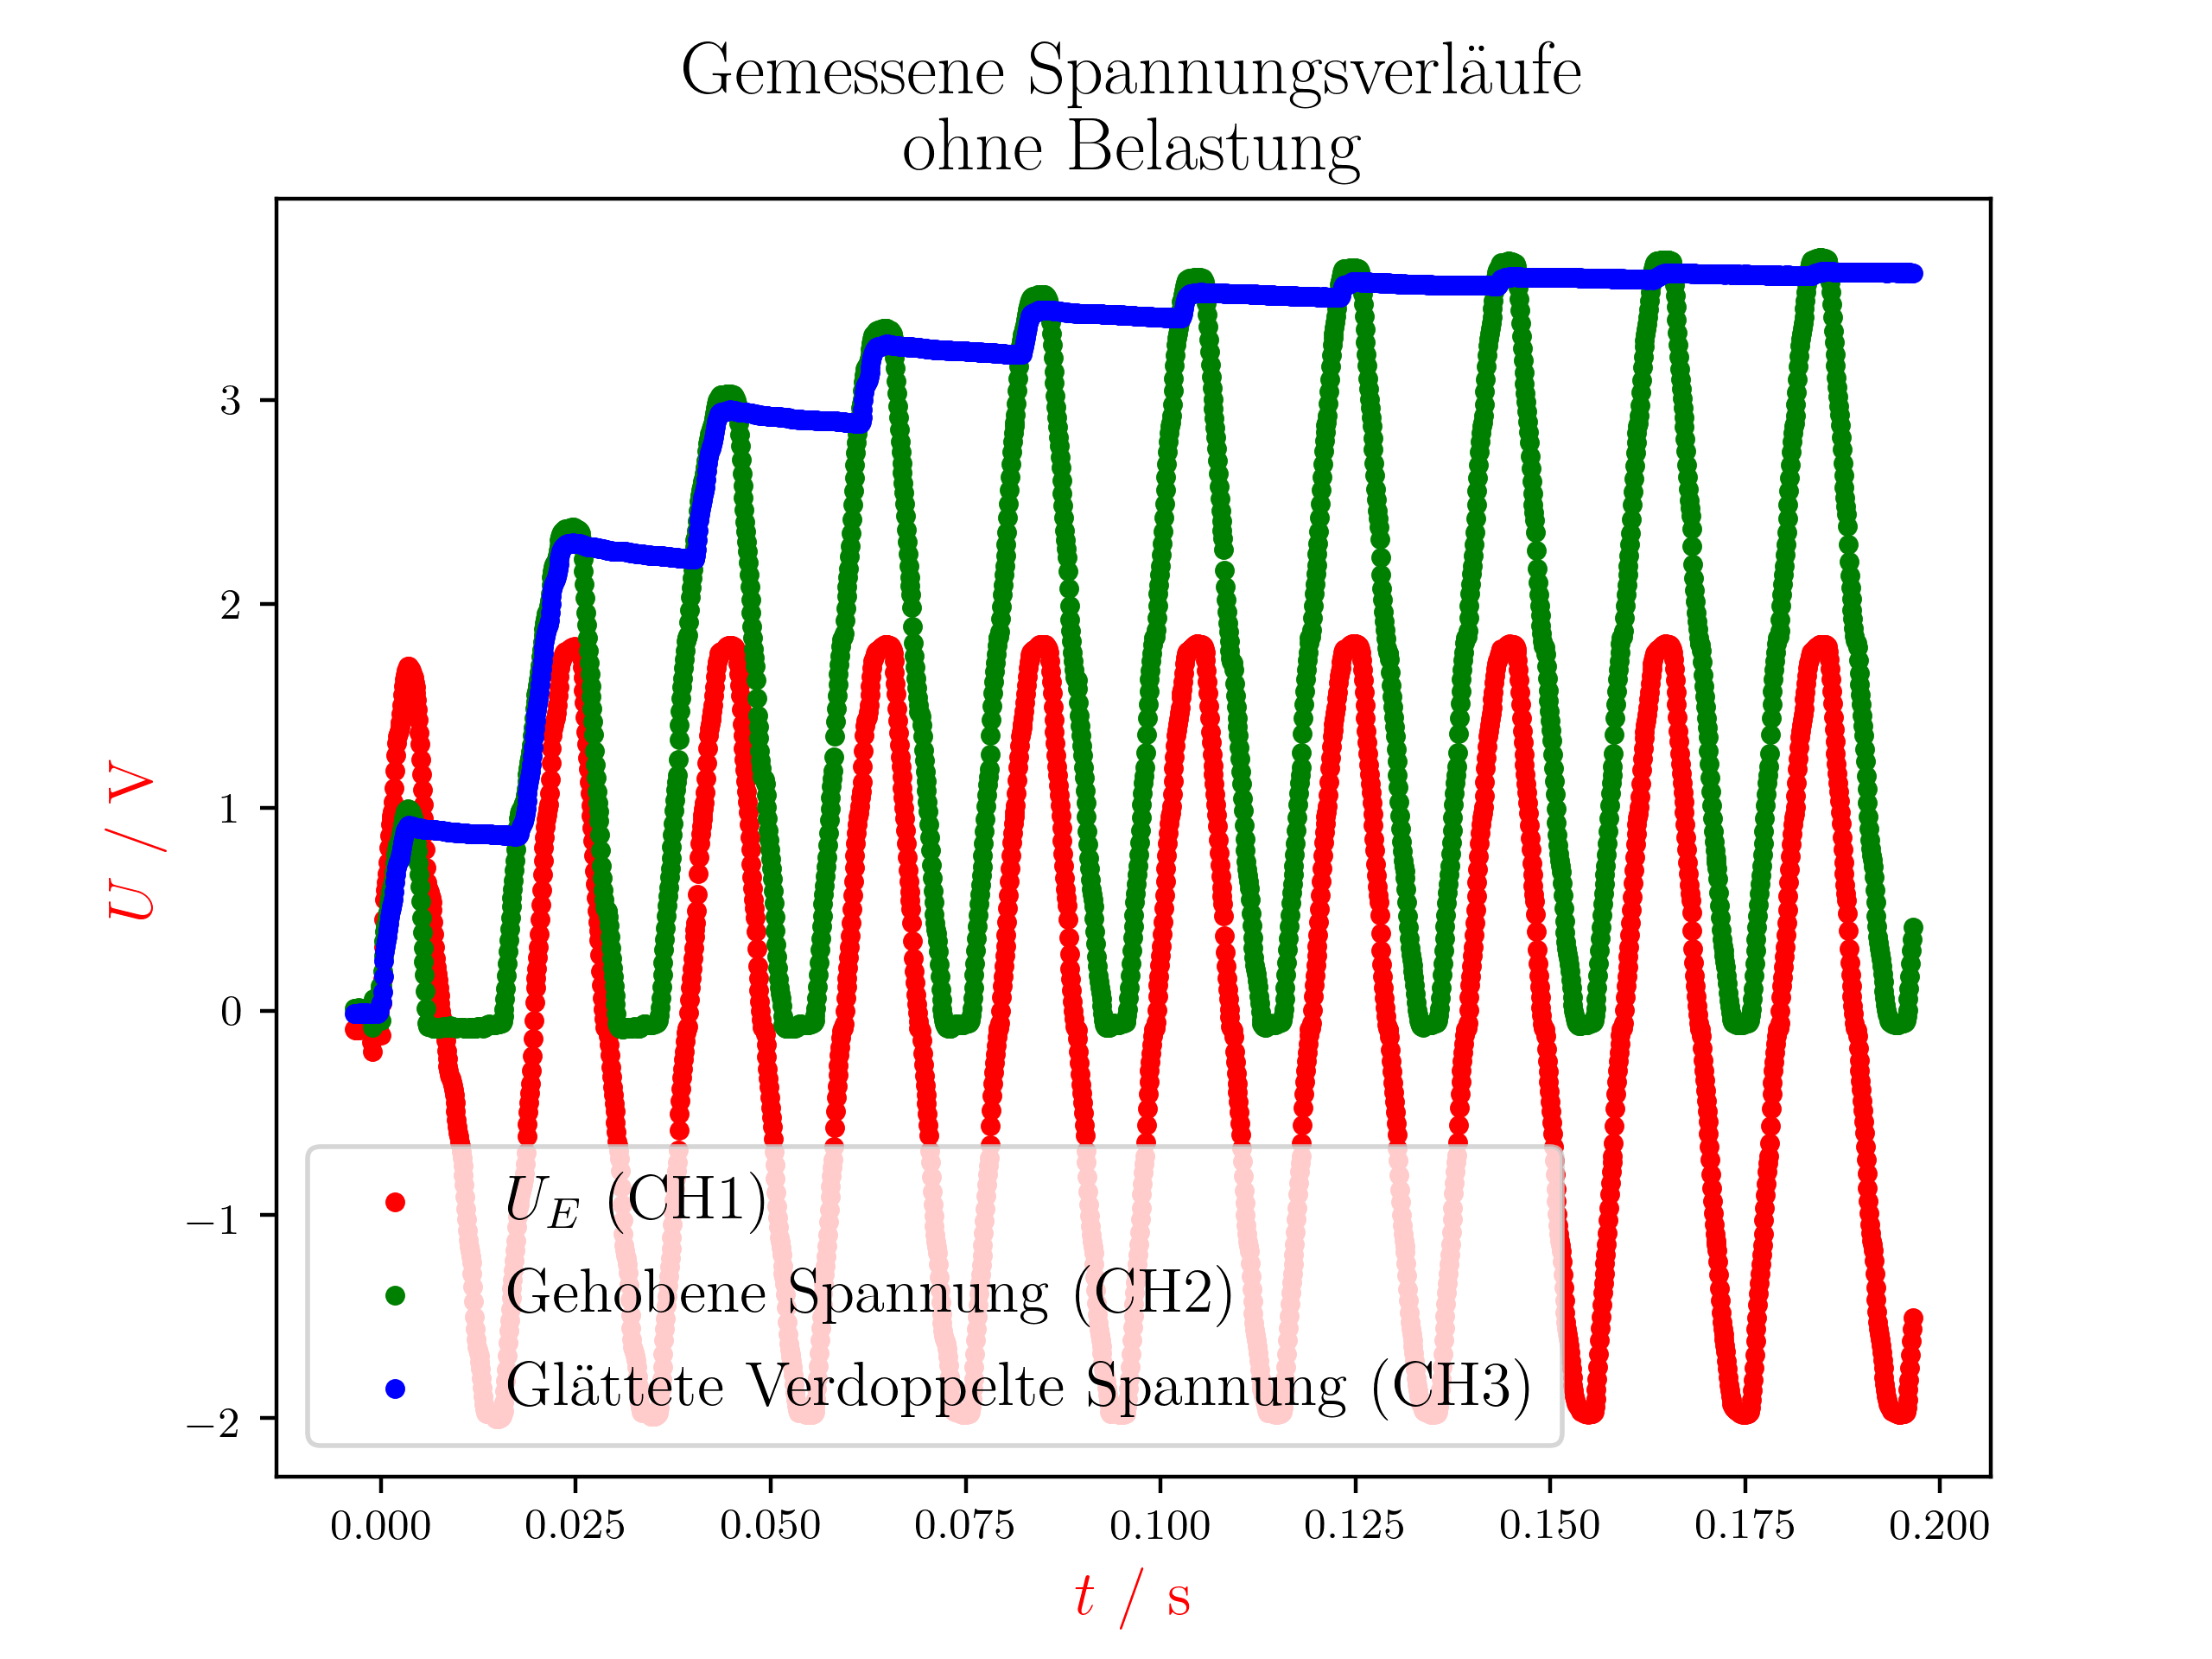
\includegraphics[width=\textwidth]{./figures/halbleiter/Versuch4/versuch4spannugenohne.png}
		\captionof{figure}{Gemessener Spannungsverlauf mit ohne Belastung}
		\label{fig:versuch4spannugenohne}
	\end{minipage}
\end{center}

Die Spannung an den Komponenten wurde dabei, wie folgt, errechnet.

\begin{equation}
	U_{C1} = U_{CH1} - U_{CH2} \quad U_{D2} = U_{CH2} - U_{CH3}
\end{equation}

Die so erhaltenen Ergebnisse sind in folgenden
\autoref{fig:spannungbauteilemit} mit Belastung und
\autoref{fig:spannungbauteileohne} ohne Belastung ersichtlich.

\begin{center}
	\begin{minipage}[t]{0.8\textwidth}
		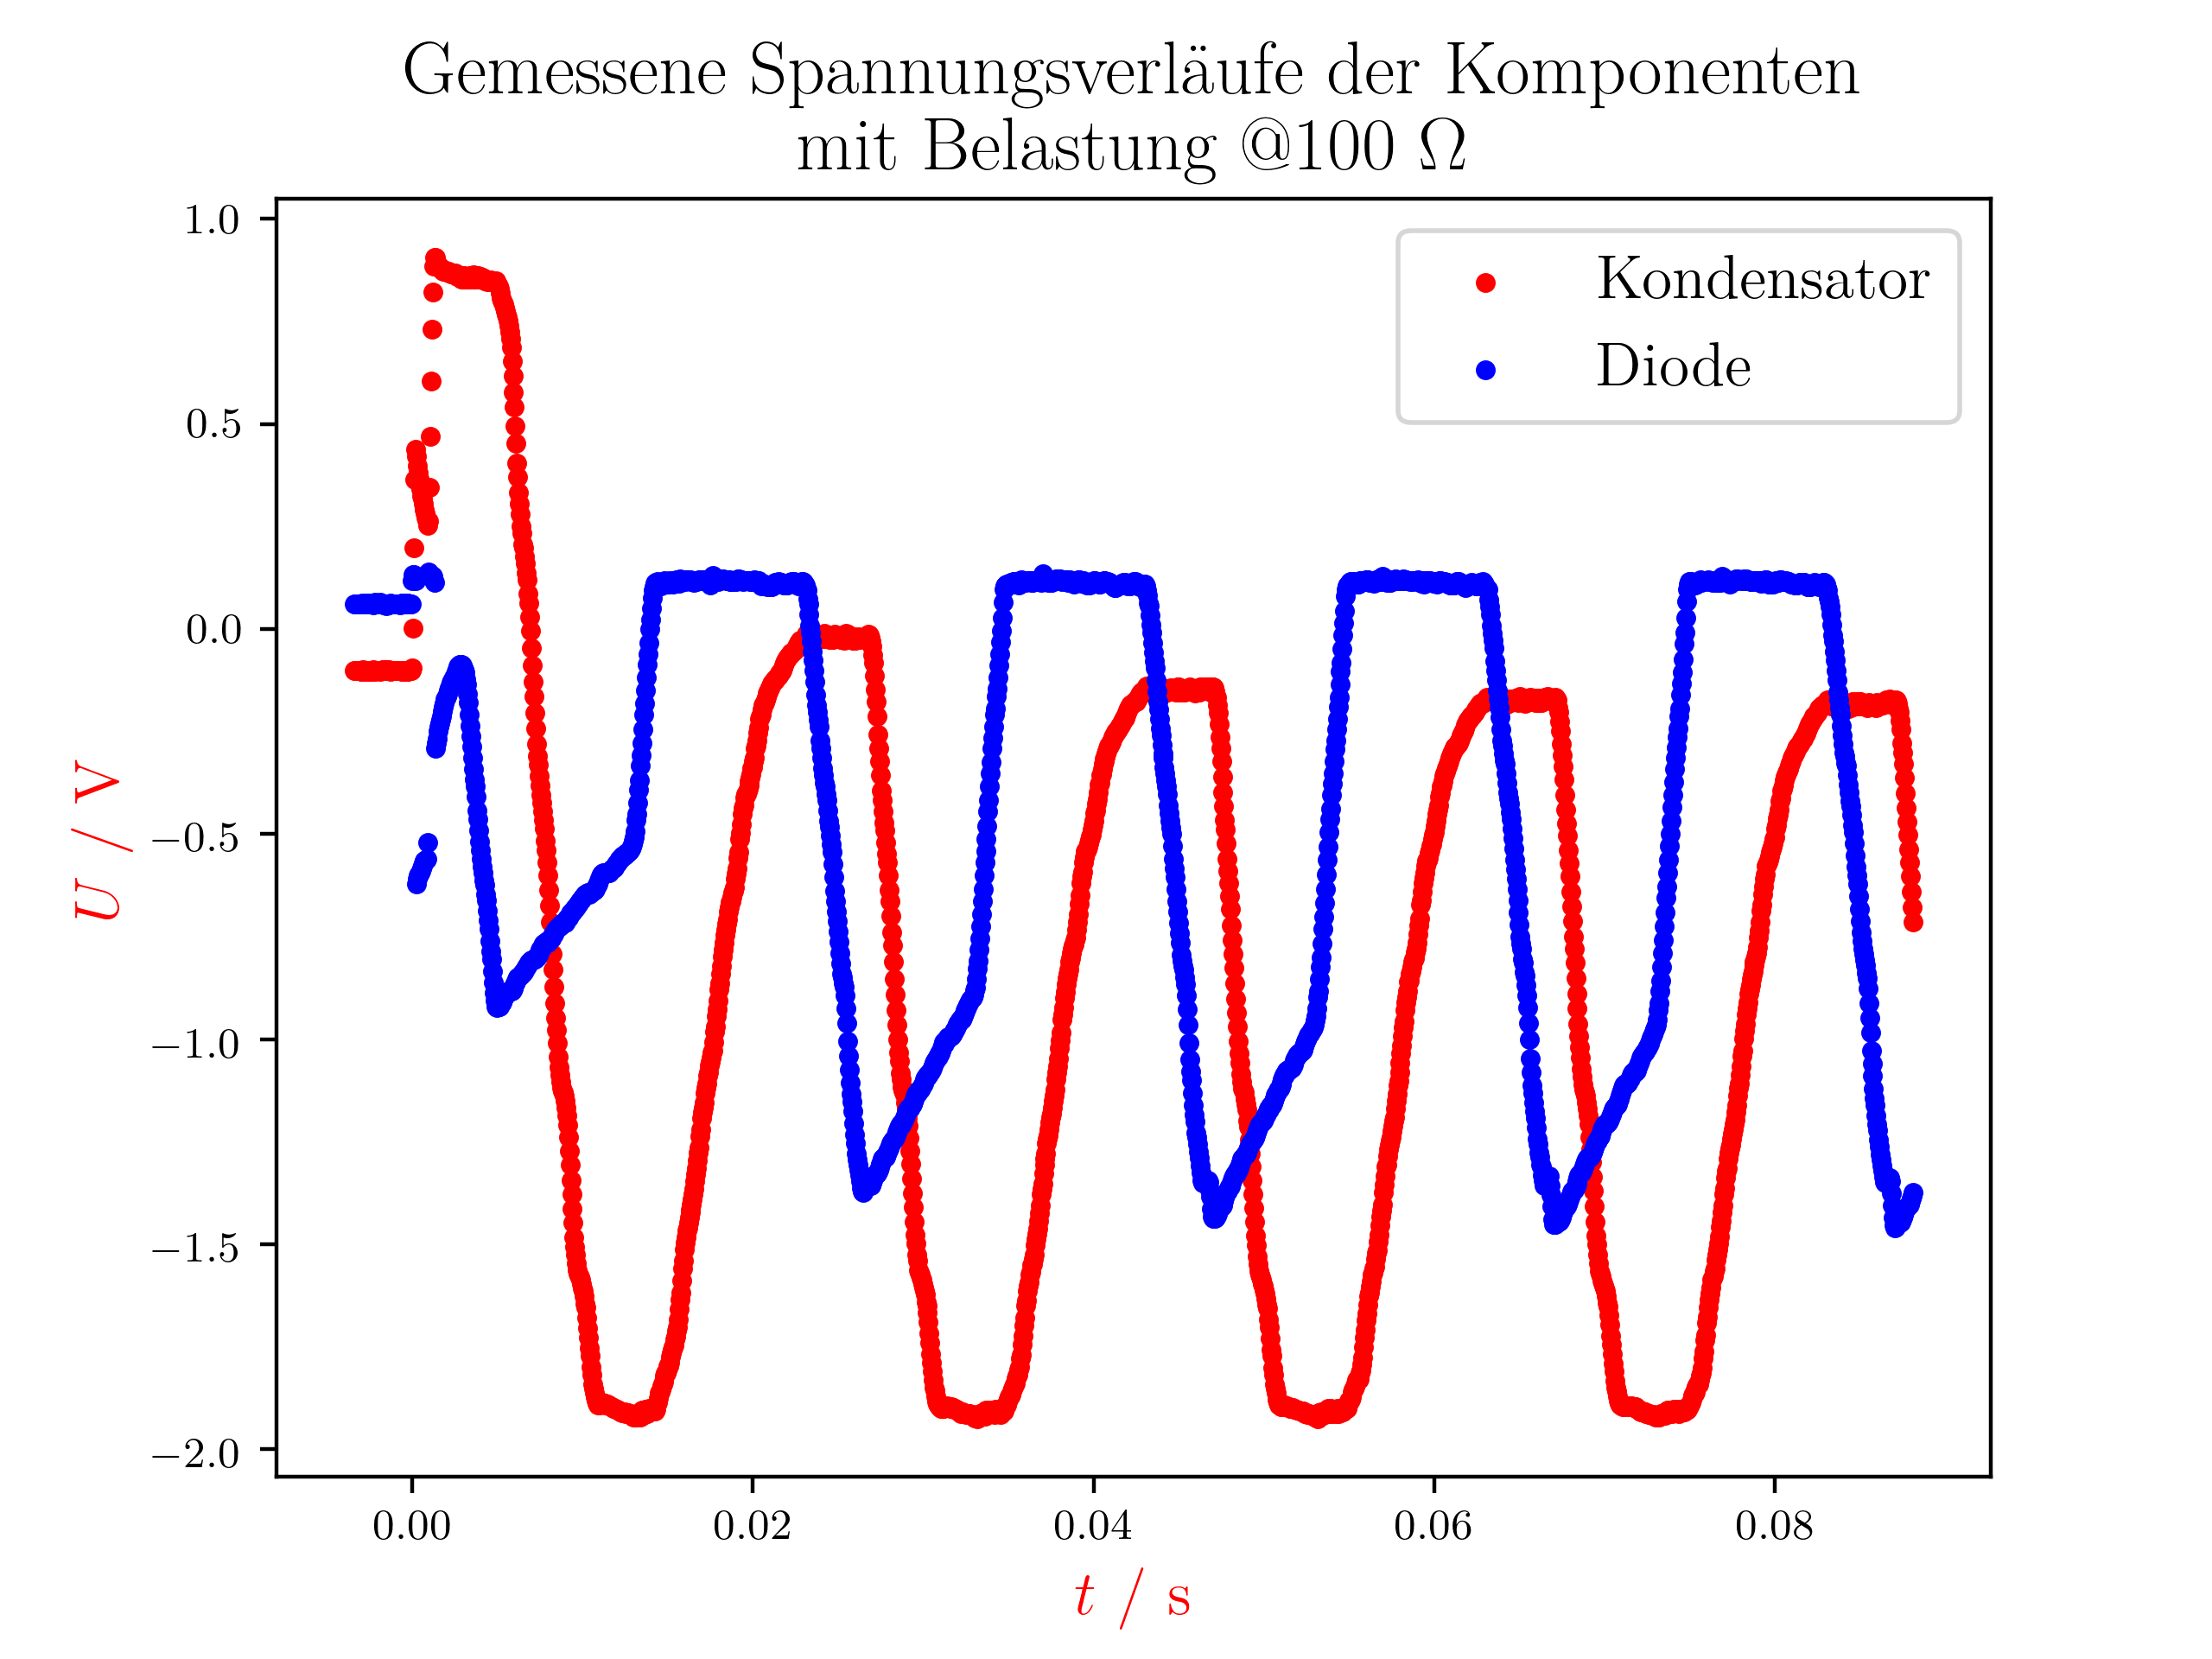
\includegraphics[width=\textwidth]{./figures/halbleiter/Versuch4/spannungbauteilemit.png}
		\captionof{figure}{Erhaltener Spannungsverlauf bei einer Belastung von \SI{99.2(11)}{\ohm}}
		\label{fig:spannungbauteilemit}
	\end{minipage}
\end{center}

\begin{center}
	\begin{minipage}[t]{0.8\textwidth}
		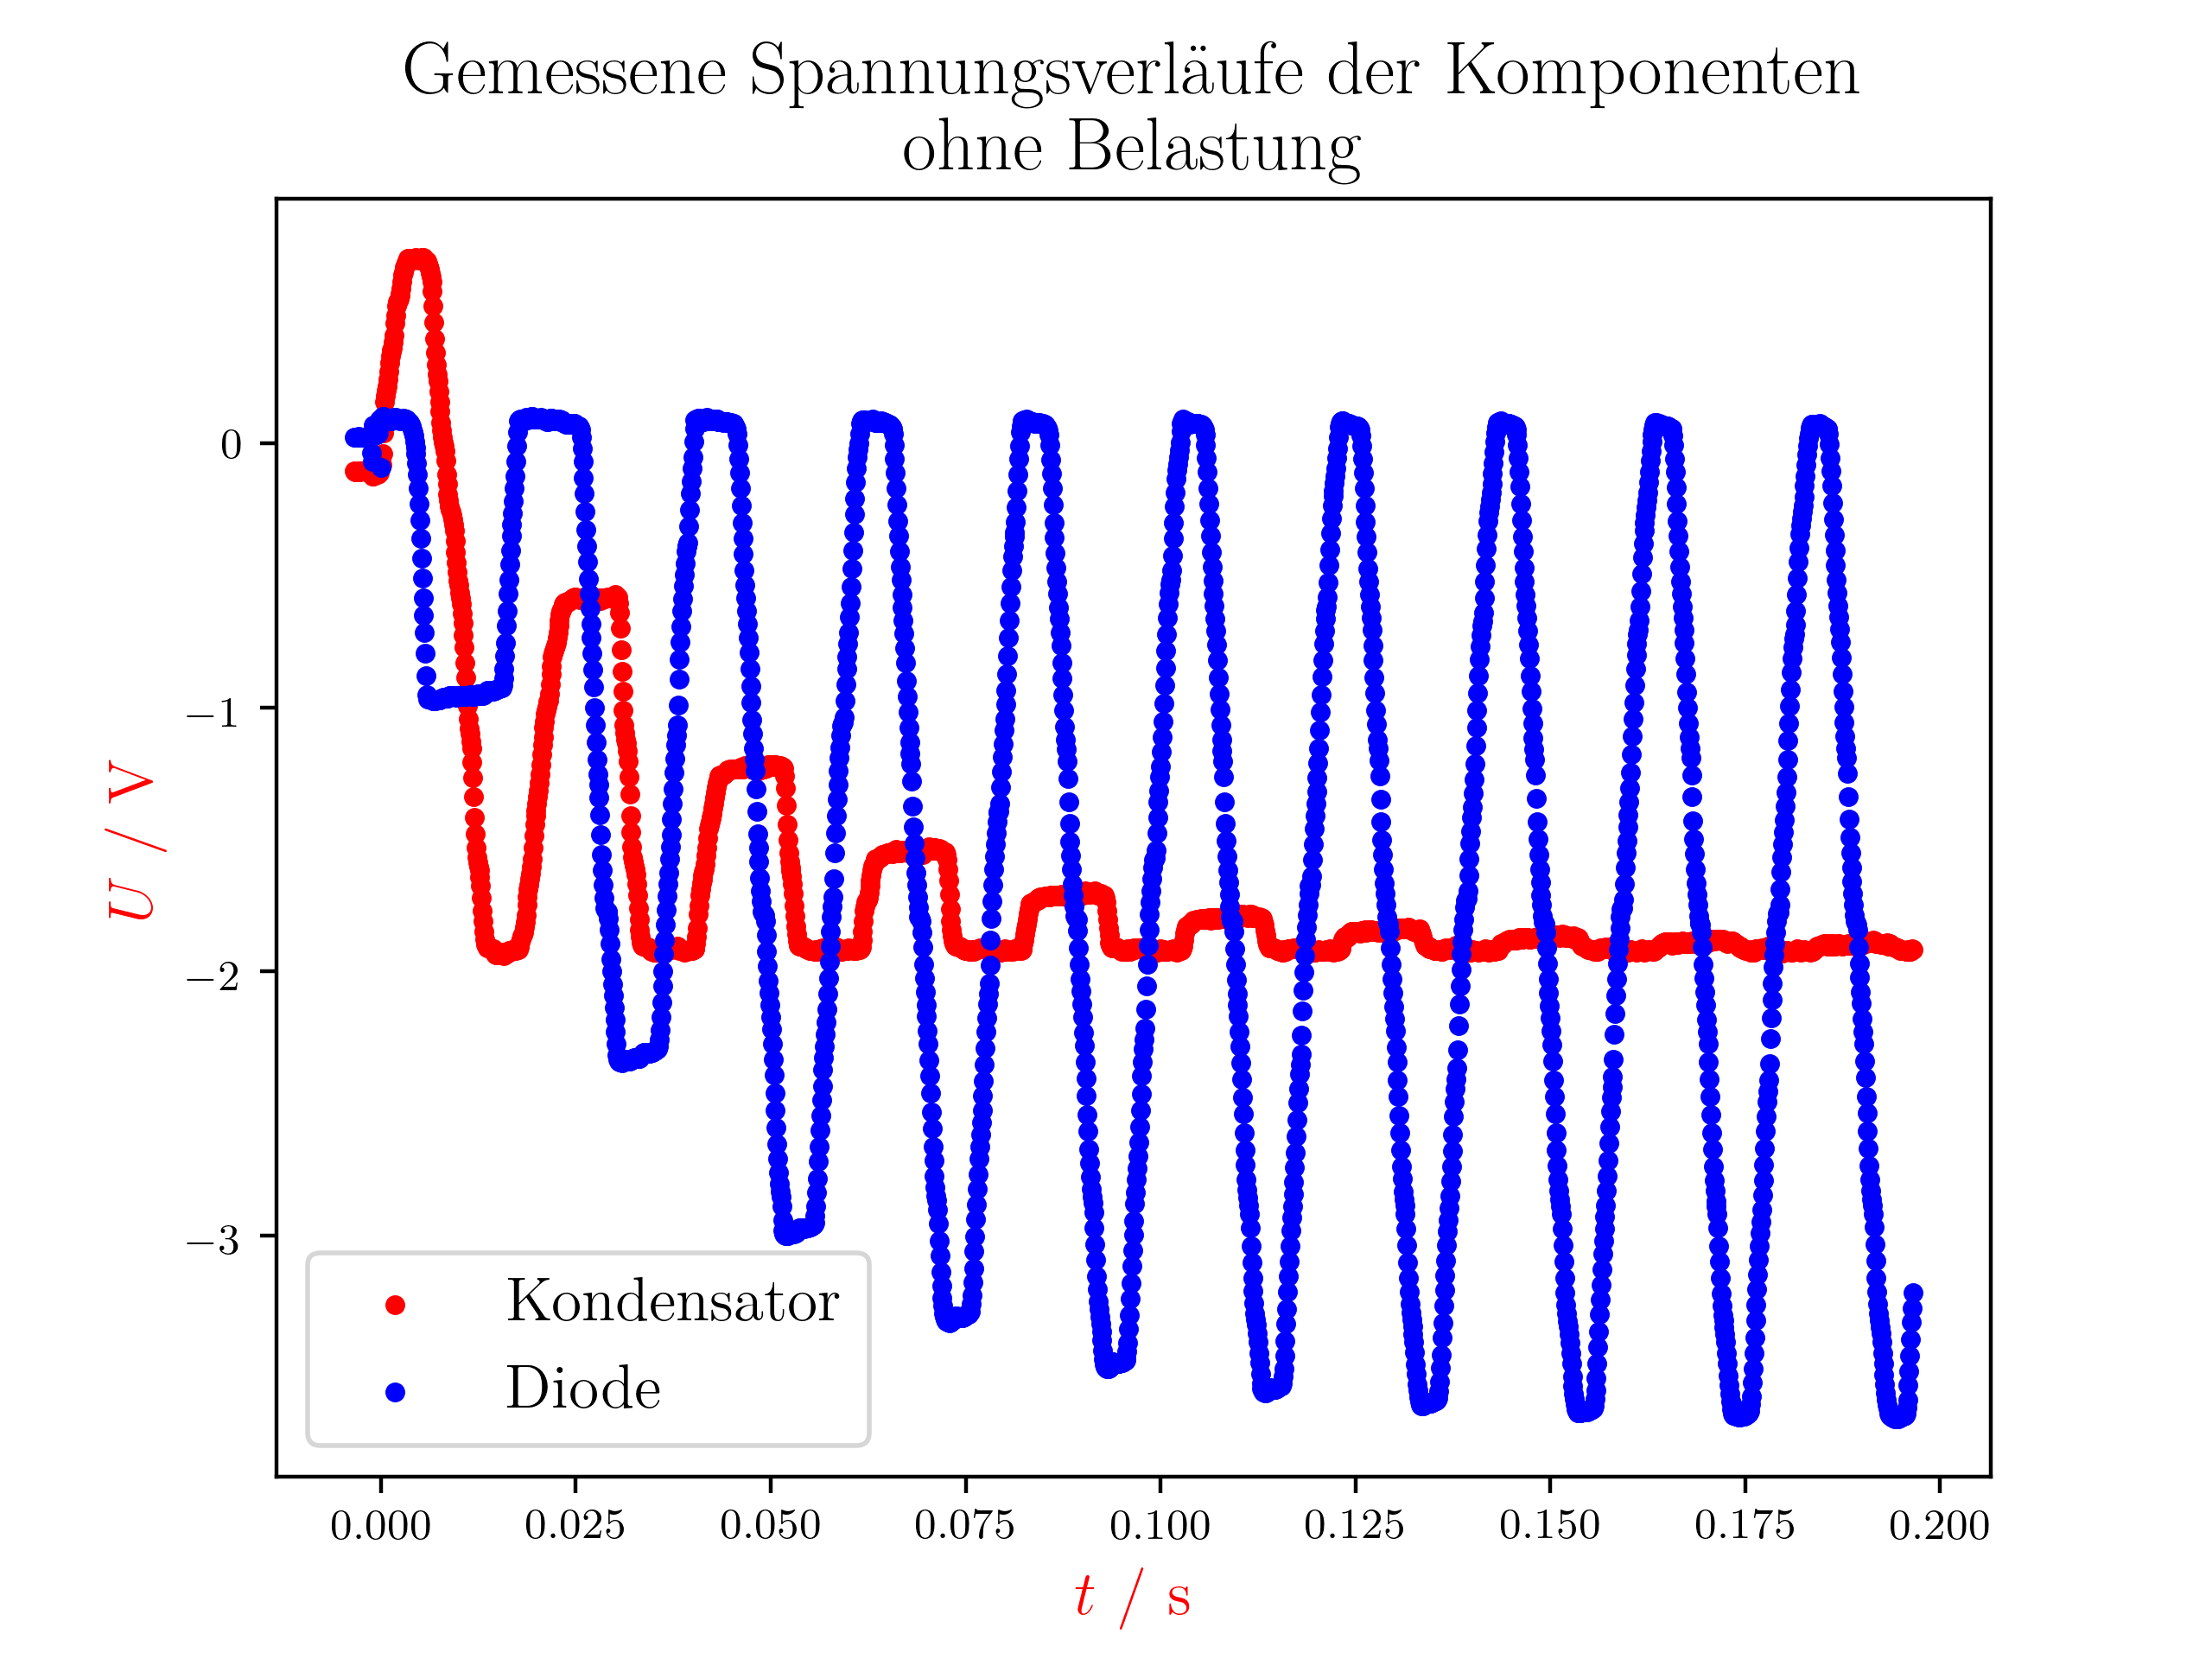
\includegraphics[width=\textwidth]{./figures/halbleiter/Versuch4/spannungbauteileohne.png}
		\captionof{figure}{Erhaltener Spannungsverlauf ohne Belastung}
		\label{fig:spannungbauteileohne}
	\end{minipage}
\end{center}


\section{Diskussion}\label{disk}


\subsection{Ermittlung der Strom-Spannungscharakteriskik einer Gleichrichterdiode}

\subsubsection{in Durchlassrichtung}

Die erhaltene Diodenkennlinie entspricht genau der Erwartung.

Auch der erhaltener Wert für die ``forward voltage`` entspricht ungefähr jenem,
der anhand des Datenblattes vorausgesagt wurde. \cite{1n4007}



\subsubsection{in Sperrrichtung}

Die typische Form der Diodenkennlinie in Sperrrichtung ist im gemessenen Bereich leider nicht sichtbar.

Wie zu erwarten war, war zwar ein kleiner negativer Strom vorhanden, der in der
Nähe des Nullpunkts bleibt. Gröbere Ausschwankungen werden, laut Datenblatt,
erst ab 1000 Volt ersichtlich. \cite{1n4007}

\vspace{2mm}

Die erhaltenen Werte entsprechen also den Erwartung, weil die
Durchbruchspannung mit der gegebenen Spannungsquelle nicht erzeugt werden kann.

Die gemessenen Sperrstromwerte sind alle kleiner als 1 mA also sind sie
deutlich kleiner als 5 mA, was den vorgegebenen Werten laut Datenblatt
entspricht. \cite{1n4007}



\subsection{Ermittlung der Strom-Spannungscharakteriskik einer Zenerdiode}

Die interpolierte Kurve der Messwerte entspricht genau der aus dem Datenblatt. \cite{1n5337}

\vspace{2mm}

Zusätzlich wurde noch die ``break down voltage`` 4.56 V , welche mit dem Cursor bestimmt wurden,
mit den Werten aus dem Datenblatt (min 4.47 V nominal 4.7 V max 4.94V)\cite{1n5337}
und verglichen. Auch dieser passen genau zu den vorausgesagten Wert.


\subsection{Untersuchung der Strom- und Spannungsverläufe mit unterschiedlichen Glättungskondensatoren und Belastungswiderständen}

Aus dem bekannten Ohm`schen Gesetz folgt:

\begin{equation}
	I = \frac{U}{R}
\end{equation}

Daraus folgt der Schluss, dass wenn der Widerstand kleiner wird, der Strom anwächst. Aus diesem Grund wird der Kondensator mehr belastet, weil so mehr Ladung entzogen wird.

\vspace{2mm}

Ein größerer Kondensator kann mehr Ladungen speichern und dadurch den Widerstand besser versorgen wodurch die Welligkeit bei den verschiedenen Widerstandsphasen kleiner wird.
Jedoch ist auch zu erwähnen, dass, bis sich das System einschwingt, eine längere Zeit benötigt wird, was in \autoref{fig:spannung_ripple_inf} ersichtlich ist.

Es kann vorkommen, dass die Frequenz zu hoch ist, sodass der Kondensator in der Periodendauer nicht vollständig geladen werden kann, wie beispielsweise in \autoref{fig:spannung_ripple_inf} ersichtlich. Die Kurve weißt eine deutlich höhere Welligkeit auf als die Kurve in \autoref{fig:spannunginf}.

\vspace{2mm}


Durch einen größeren Widerstand fließt mehr Strom, wie es in \autoref{fig:strominf}, \autoref{fig:strom1509} und \autoref{fig:strom100} ersichtlich ist.

Wenn das System eingeschwungen ist, wird die Spannung der Diode negativ, wie in allen Abbildungen der Spannung ersichtlich.

\vspace{2mm}

Am Stromverlauf wird auch sichtbar, dass wenn die Spannung in der Diode absinkt, der Strom beginnt durch den Kondensator zu fließen. Dadurch entlädt sich dieser und beginn den Spannungsabfall zu kompensieren.

Die Welligkeit nimmt ab, wenn die Kapazität des Kondensators größer wird, weil dieser den Verbrauch besser deckten kann.
Weil ein großer Kondensator mehr Ladungen halten kann, kann er für längere Zeit bei gleichen Strom, oder bei höheren Strom für die gleiche Zeit, die Spannung erhalten.

\vspace{2mm}

Bei gar keiner Belastung fließt zwar Strom, aber nur aufgrund des Rests von Kondensatoren und Dioden, weil diese nicht perfekt sind, wie auch in \autoref{fig:strominf} ersichtlich.



\subsection{Untersuchung der Spannungsverläufe in einer Spannungsverdopplerschaltung}



Das Phänomen der Spannungsverdopplung lässt sich in 2 Phasen aufteilen.

Die 1. Phase ist die Phase, wo eine positive Spannung in Durchlassrichtung über die Diode 1 anliegt.

In Phase 2 wird über die Diode 1 eine Negative Spannung angelegt.

\vspace{2mm}

In Phase 1 ist der einzige Weg für Stromfluss der Weg über Diode 1 und Kondensator 1 zurück zum Transformator, wodurch sich dieser Kondensator auflädt.
Dies gilt, weil alle anderen Wege durch Diode 2 blockiert sind.

\vspace{2mm}

Bei Phase 2 ist der einzige Weg für den Stromfluss über Kondensator 1, Diode 2 und Kondensator 2, wobei zusätzlich zur positive Spannung vom Trafo, noch die Spannung des geladenen Kondensators C1 hinzukommt, den Kondensator C2 zu laden.

\vspace{2mm}

Diese 2 Phasen wechseln sich so oft ab, bis C1 zur Eingangsspannung geladen ist und C2 die doppelte Spannung von C1 hat, wodurch nun eine Spannungsverdopplung entsteht.

Dabei ist zu erwähnen, dass die Verdoppelung durch die Addition der Spannung von C1 und den Trafo ermöglicht wird.

%Punkte bei 5.4 anschreiben abb 23

\vspace{2mm}

Diese erklärte Schaltung zeigt nur den Fall von keiner Belastung.
Gibt es jedoch eine Belastung so gibt es einen Weg für den Kondensator, sich über den Widerstand zu entladen, wie in \autoref{fig:versuch4spannugenmit} ersichtlich.

\vspace{2mm}

Eine Verbesserung der Schaltung wäre, einen größeren Widerstand zu verwenden, wodurch die Belastung auf den Kondensator geringer wird, oder eine Vergrößerung der Kapazität der Kondensatoren.

\vspace{2mm}

Wie zu erwarten war, pendelt sich die Kondensatorspannung bei einen bestimmten
Wert ein, siehe \autoref{fig:spannungbauteileohne}. Dies ist jedoch nicht im
Spannungsverlauf des Kondensators beim belasteten Fall ersichtlich, siehe
\autoref{fig:spannungbauteilemit}.


Der Spannungsverlauf über die Diode baut sich beim unbelasteten Fall auf, wie
in \autoref{fig:spannungbauteileohne} ersichtlich. Beim belasteten Fall jedoch,
wird erkennbar, dass der maximale Spannungsunterschied einigermaßen konstant
bleibt, da es aufgrund des Entladens des Kondensators am Widerstand, keine
Möglichkeit gibt, dass sich die Spannungen des Kondensators und des Trafos
addieren.


\subsection{Verbesserungsvorschläge}


Ein Verbesserungsvorschlag wäre, die Tastkabel für alle Versuche zu verwenden,
weil das Oszilloskop darauf eingestellt ist, den 10x Modus zu verwenden.

Wenn weiterhin die Bananenbuchsenstecker verwendet werden sollen, wäre es
besser die entsprechenden Adapterstücke zu verwenden, um so die Koaxialkabel zu
vermeiden.

%noch ideen?

\section{Zusammenfassung}

Die Diodenkennlinie in Durchlassrichtung stimmt mit mit der Referenzlinie aus dem Datenblatt überein.
In Sperrrichtung wurde nur ein kleiner Strom, der viel kleiner als der Durchlassstrom war, aufgewendet. Dadurch konnte die charakteristische Linie nicht erzeugt werden, was auch zu erwarten war.

\vspace{2mm}

Auch der direkte Vergleich der erhaltenen Diodenkennlinie der Zenerdiode stimmt mit jener aus dem Datenblatt überein.
Auch die verglichenen Werte der ``break down voltage`` und der ``forwarding voltage`` stimmen mit dem Datenblatt überein.

\vspace{2mm}

Wie anhand der Skizzen und Werten in den Diagrammen klar ersichtlich ist, nimmt
die Welligkeit bei einem höheren Widerstand, sowie einer Erhöhung der
Kapazität, ab.


\newpage

\printbibliography
\listoffigures
\listoftables
\end{document}



